\documentclass[a4paper,12pt]{extarticle}
\usepackage{setup}

\begin{document}

  \pagestyle{plain}  % Disable header content.

  % ===== Cover =====

  \begin{titlepage}
    \begin{center}
      \vspace*{1cm}  % Respects page break.

      \Large{\textsc{\textcolor{maroon}{Aristotle University of
Thessaloniki\\Department of Informatics}}}

      \vspace{1.5cm}

      \Large{\textsc{Postgraduate Thesis}}

      \vspace{1cm}

      \line(1,0){415}
      \vspace{5.5mm}
      {\fontsize{20.74}{24}\selectfont\bfseries
        \parbox{415pt}{\centering Computational Assessment of a Scalable, Reproducible \& Interpretable Clustering Workflow in the Natural Genome Space}
      }

      \vspace{2mm}
      \line(1,0){415}
    \end{center}
    \vspace{3cm}
    \begin{minipage}{\textwidth}
      \large{\textbf{\textit{Author}}}
      \hfill
      \large{\textbf{\textit{Supervisor}}}
      \\
      \textcolor{maroon}{\large{Apostolos M. \textsc{Dimoulakis}}}
      \hfill
      \textcolor{maroon}{\large{Prof. Christos A. \textsc{Ouzounis}}}
    \end{minipage}

    \vspace{\fill}

    \begin{center}
      \textbf{\large{?\{month\} ?\{day\}, 2026}}
    \end{center}
  \end{titlepage}
  
  % ===== Abstract =====

  \pagenumbering{roman}
  
  \pagestyle{headerpage}
  
  \subsection*{%
    \center Abstract
  }
  
  \textbf{Background}: Protein clustering is an essential data reduction technique for managing the scale of modern genomic datasets. As sequencing technologies advance, the volume of publicly available protein sequences has grown exponentially, yet the computational resources required for downstream functional and structural analysis often lag behind.

  \textbf{Problem}: The central problem addressed in this thesis is whether a single compute node can handle the growing scale of genomic data for graph-based protein clustering.

  \textbf{Method}: Using the Markov Cluster Algorithm (MCL) and its high-performance variant HipMCL, we assessed performance across datasets ranging from 3,500 to 82 million sequences drawn from UniProtKB reference proteomes. To enable convenient and reproducible execution, we developed \texttt{bioscflow}, a reproducible workflow implementing the entire pipeline.

  \textbf{Results}: Here we show that MCL scales to 82 million sequences on a single node, completing within 2--3 days using approximately 440 GiB of memory, while HipMCL is impractical beyond 3 million sequences in the same environment due to excessive memory overhead and convergence failures. Qualitative analysis --- including taxonomic purity assessment, graph-based community validation, and structure superimposition of AlphaFold-derived models --- confirms that the largest clusters are taxonomically coherent and structurally consistent.

  \textbf{Conclusion}: The workflow meets its design priorities: scalability, as MCL handles production-scale data; reproducibility, through \texttt{bioscflow} with versioned components such as MCL; and interpretability, via alignment-based graph edges with no black-box embeddings. These findings establish a reliable computational baseline for the StratoCluster initiative and provide a foundation for future GPU-accelerated and distributed clustering efforts.

  \vspace{0.3cm}

  \noindent{\small \textcolor{black!80}{\textbf{Keywords}: protein clustering, Markov Cluster Algorithm, HipMCL, sequence similarity networks, scalability, reproducibility, interpretability, AlphaFold, StratoCluster}}

  \vspace{\fill}

  \subsection*{%
    \center Περίληψη
  }

%  Η ομαδοποίηση πρωτεϊνών αποτελεί μια ουσιαστική τεχνική μείωσης δεδομένων για
%  τη διαχείριση της κλίμακας των σύγχρονων γονιδιωματικών συνόλων δεδομένων. Η
%  παρούσα διπλωματική εργασία διερευνά την πρακτική επεκτασιμότητα,
%  αναπαραγωγιμότητα και ερμηνευσιμότητα ενός υπάρχοντος workflow ομαδοποίησης
%  βασισμένου σε γράφο που αναπαριστά τις ομοιότητες πρωτεϊνικών αλληλουχιών
%  (PSSN) και οι υπολογισμοί βασίστηκαν σε έναν μόνο κόμβο υπολογισμού.
%  Χρησιμοποιώντας τον αλγόριθμο Markov Cluster Algorithm (MCL) και την υψηλής
%  απόδοσης παραλλαγή του HipMCL, πραγματοποιήσαμε συστηματική συγκριτική
%  αξιολόγηση της απόδοσης σε σύνολα δεδομένων που κυμαίνονται από 3500 έως 82
%  εκατομμύρια αλληλουχίες, προερχόμενα από τα reference proteomes της UniProtKB
%  --- ένα μεγάλο υποσύνολο του φυσικού γονιδιωματικού χώρου. Για τη διευκόλυνση
%  της αναπαραγωγιμότητας, αναπτύξαμε το εργαλείο \texttt{bioscflow}, μια
%  συμπαγή υλοποίηση ολόκληρου του workflow. Τα αποτελέσματά μας δείχνουν ότι το
%  MCL κλιμακώνεται έως και 82 εκατομμύρια αλληλουχίες σε έναν μόνο κόμβο υπολογισμού,
%  ολοκληρώνοντας την εκτέλεση σε 2–3 ημέρες με κατανάλωση μνήμης περίπου 440
%  GiB, ενώ το HipMCL είναι μη πρακτικό πέραν των 3 εκατομμυρίων αλληλουχιών στο
%  ίδιο περιβάλλον, λόγω υπερβολικής κατανάλωσης μνήμης και αποτυχιών σύγκλισης.
%  Η ποιοτική ανάλυση --- περιλαμβανομένης της μετρικής purity, της επικύρωσης κοινοτήτων του γράφου, και του superimposition των πρωτεϊνικών δομών (AlphaFold) 
%  --- επιβεβαιώνει ότι οι μεγαλύτερες ομάδες
%  (clusters) είναι ταξινομικά συνεκτικές και δομικά συνεπείς. Η ροή εργασίας
%  ανταποκρίνεται στις σχεδιαστικές της προτεραιότητες: επεκτασιμότητα, καθώς το
%  MCL διαχειρίζεται δεδομένα παραγωγικής κλίμακας· αναπαραγωγιμότητα, μέσω του
%  \texttt{bioscflow} με εκδόσιμα συστατικά (π.χ. MCL commit)· και ερμηνευσιμότητα,
%  μέσω γραφικών ακμών που βασίζονται σε στοίχιση αλληλουχιών, χωρίς μαύρα
%  κουτιά. Τα ευρήματα αυτά θεμελιώνουν μια αξιόπιστη υπολογιστική γραμμή βάσης
%  για την πρωτοβουλία StratoCluster και παρέχουν μια βάση για μελλοντικές
%  προσπάθειες επιτάχυνσης μέσω GPU και κατανεμημένης επεξεργασίας.
  
  
  \vspace{\fill}
  
  \cleardoublepage

  % ===== Thesis Committee & Acknowledgements =====
  
  \vspace*{\fill}
  
  \subsection*{%
    Thesis Committee Members
  }

  \vspace{3mm}

  {
    \setlength{\tabcolsep}{3.2mm}
    \begin{tabular}{r l}
      Prof. Christos Ouzounis, Professor & Department of Informatics
      \\[2mm]
      Committee, Supervisor & Aristotle University of Thessaloniki
      \\[4mm]
      Prof. Eleftherios Angelis, Professor & Department of Informatics
      \\[2mm]
      Committee & Aristotle University of Thessaloniki
      \\[4mm]
      Prof. Grigorios Tsoumakas, Professor & Department of Informatics
      \\[2mm]
      Committee & Aristotle University of Thessaloniki
    \end{tabular}
  }

  \vspace{3cm}

  \subsection*{%
    Acknowledgements
  }

  I would like to sincerely thank the committee members for their guidance and support, and my colleague Anastasios Karydis for his cooperation and technical assistance throughout this research project.

  \vspace{\fill}

  \cleardoublepage

  % ===== Table of Contents =====

  \tableofcontents
  \cleardoublepage

  % ===== Glossaries =====

  \subsection*{%
    \centering Glossary
  }
  
  The following definitions are included to support the reader's understanding of concepts referenced in this thesis.
  
  \subsubsection*{%
    \textcolor{gray}{Molecular Chemistry}
  }

  \begin{description}[leftmargin=1.2em]
    \item[Molecule]: A chemically bonded group of two or more atoms that forms a discrete, electrically neutral unit.
    \item[Covalent Bond]: The sharing of electron pairs between atoms. This forms the fundamental structure of molecules. This is the strongest type of bond and the backbone of amino acids and proteins.
    \item[Monomer]: A molecule that can form covalent bonds with two or more other molecules in a stable and repeating pattern, leading to a larger molecule called polymer.
    \item[Monomeric Unit]: The largest constitutional unit of a macromolecule that corresponds to a single monomer.
    \item[Amino Acid]: A monomer that contains both \(-\text{NH}_2\) and \(-\text{COOH}\). Here, the notation \(-X\) means that there is a covalent bond between some unspecified molecule and molecule \(X\) (e.g., \(\text{NH}_2\)). An amino acid can link together with other amino acids to form a protein.
    \item[Macromolecule]: A molecule of high relative molecular mass, the structure of which essentially comprises the multiple repetition of units derived, actually or conceptually, from molecules of low relative molecular mass.
    \item[Polymer]: A polymer is a large molecule made up of repeating monomer units covalently bonded together.
    \item[Residue]: A molecular unit that constitutes part of a macromolecule after covalent incorporation of a monomer, retaining the core atomic structure of the original monomer but lacking the atoms lost during bond formation.
  \end{description}
  
  \subsubsection*{%
    \textcolor{gray}{Genomics}
  }
  
  \begin{description}[leftmargin=1.2em]
    \item[Domain \textnormal{or} Superkingdom]: The broadest taxonomic rank in the tree of life, above kingdom, grouping organisms based on fundamental cellular and genetic characteristics. The domains is classified as one of the following organism classes: Bacteria, Archaea or Eukaryota.
    \item[DNA]: Long, double-stranded molecule that stores an organism's genetic information.
    \item[mRNA]: Carries the genetic instructions from DNA. Ribosomes read its codons to determine the amino-acid sequence.
    \item[tRNA]: A type of RNA that brings amino acids to the ribosome from the cytoplasm (amino acids float abundantly); each has an anticodon that matches a specific mRNA codon.
    \item[Codon]: A subsequence of 3 bases from the mRNA sequence (alphabet).
    \item[Anticodon]: Attaches to a codon (3 bases to 3 bases) to receive the signal that specifies the amino acid. Each anticodon has at least one complementary/matching codon that triggers the release of the carried amino acid.
    \item[Prokaryota]: Single-cell organisms without a true nucleus or membrane-bound organelles. Prokaryota are either bacteria or archaea.
    \item[Bacteria]: Prokaryotic, unicellular organisms without a nucleus.
    \item[Archaea]: Prokaryotic organisms with distinct biochemistry from bacteria.
    \item[Eukaryota]: Organisms with eukaryotic cells, including animals, plants, fungi, and protists.
    \item[Protein (Sequence)]: A chain of amino acids that can fold into a functional structure; in this thesis, represented as its amino acid residue sequence (i.e., the protein's primary structure).
    \item[Reference Protein Sequence]: A protein sequence that represents a set of similar sequences.
    \item[Protein Primary Structure]: The sequence of covalently bonded amino acid residues of a protein.
    \item[Genome]: The complete set of genetic material in an organism, including all of its DNA (or RNA in some viruses), encompassing all genes as well as non-coding sequences.
    \item[Gene]: A subsequence of DNA that encodes a functional product, such as a protein or functional RNA. One gene may encode multiple proteins.
    \item[Motif]: A recurring, biologically meaningful sequence pattern associated with a specific structural or functional role. Motifs are typically short and locally conserved, but allow variability in the form of substitutions and, in some cases, insertions or deletions.
    \item[Proteome]: The complete set of proteins encoded by an organism's genome.  
    \item[Reference Proteome]: A representative, non-redundant subset of a proteome, used as a computational baseline or ground truth.
    \item[Phylogeny]: The evolutionary history and relationships among species or genes, often represented as a tree or hierarchy, based on genetic or protein sequences.
    \item[Isoforms]: A set of sequences are isoforms when a member sequence (i.e., an isoform) is derived from the same gene (DNA), differing from the canonical sequence due to alternative splicing (in Eukaryota) or related processing. Isoforms do not guarantee equivalent or similar functionality.
    \item[Homology]: The existence of shared ancestry between sequences or structures; homologs (i.e., collections of homologous sequences) are derived from a common ancestor.
    \item[Sequence Alignment]: The process of arranging two or more biological sequences (DNA, RNA, or protein) so that residues that are homologous or functionally/evolutionarily equivalent appear in the same position inside the sequences.
    \item[Alignment Coverage]: When two sequences are aligned, the alignment coverage is the fraction of the shorter sequence that participates in the alignment.
    \item[Sequence Identity]: Sometimes called \textit{percentage identity}, is the fraction of a sequence that matches exactly the other sequence after a pair of sequence is aligned.
    \item[Protein Sequence Similarity Network (PSSN)]: A weighted graph where each vertex is a protein sequence and the edge-weight is a measure of pairwise similarity.
    \item[Compositional Bias]: The significant deviation of a motif's composition from the background amino acid distribution.
    \item[Ribbon Diagram]: A schematic 3D representation of a protein composed of folded secondary structure elements, where \(\alpha\) helices appear as spirals, \(\beta\) strands as arrows, and loops as tubes.

    \begin{figure}[htbp]
      \centering
      \begin{minipage}{0.43\linewidth}
        \centering
        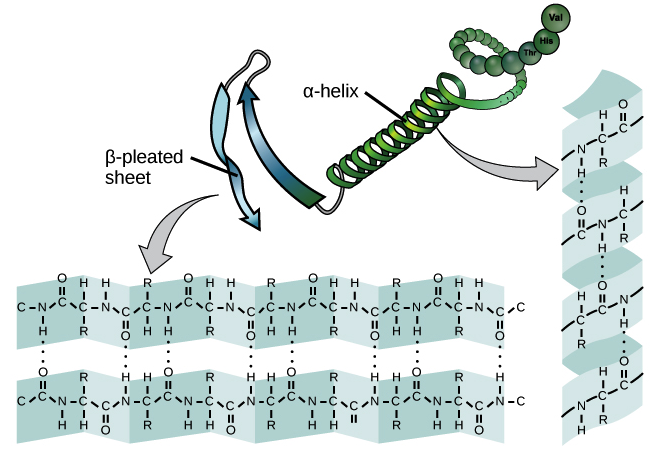
\includegraphics[width=\linewidth]{asset/secondary_struct.png}
        \caption*{Image adapted from \textit{Orders of Protein Structure} by Khan Academy, available under a Creative Commons BY-NC-SA 4.0 License.}
        \label{fig:secondary_struct}
      \end{minipage}
    \end{figure}

  \end{description}

  % Institutions, databases, frameworks, funds, software systems.
  \subsubsection*{%
    \textcolor{gray}{Infrastructure}
  }

  \begin{description}[leftmargin=1.2em]
    \item[Universal Protein Resource (UniProt)]: A public database\footnote{\url{https://ftp.uniprot.org/pub/databases/uniprot}} of protein information. It is the product of a collaboration between the European Bioinformatics Institute (EBI), the SIB Swiss Institute of Bioinformatics, and the Protein Information Resource (PIR). UniProt comprises three databases, namely UniProtKB, UniRef and UniParc.
    \item[UniProt Knowledgebase (UniProtKB)]: Central access point for extensively curated protein information, including function, classification and cross-references.
    \item[AlphaFold Protein Structure Database]: A public database of three-dimensional protein structure predictions. It is a collaboration between EMBL-EBI and DeepMind, providing estimated three-dimensional arrangement (tertiary structure) for over 200 million proteins, covering nearly all known organisms.
  \end{description}
  
  \subsubsection*{%
    \textcolor{gray}{Uncategorized}
  }

  \begin{description}[leftmargin=1.2em]
    \item[\(\mathbb{N}\)]: The set of natural numbers \(\{ 0, 1, 2, \dots  \}\).
    \item[\(\mathbb{R}\)]: The set of real numbers.
    \item[\(\mathscr{S}^*\)]: For a set \(\mathscr{S} \subseteq \mathbb{R}\), the symbol \(\mathscr{S}^*\) denotes a set containing all elements of \(\mathscr{S}\) except from \(0\).
    \item[\(\mathcal{M}^e\)]: For a matrix \(\mathcal{M}\) and some \(e \in \mathbb{N}^*\), \(\mathcal{M}^e\) is defined as
    \[
      \mathcal{M}^e = \underbrace{\mathcal{M} \cdot \mathcal{M} \cdot \hdots \cdot \mathcal{M}}_{e \text{ terms}} .
    \]
    where \(\cdot\) is the matrix multiplication function.
    \item[Clustering]: For a given set \(\mathscr{V}\), clustering is the task of finding a pairwise disjoint collection of subsets of \(\mathscr{V}\) based on structural or semantic similarities \(\mathscr{V}\) (e.g., based on the Euclidean distance function). Each subsequent subset of \(\mathscr{V}\) is a \textit{cluster}.
    \item[Community Detection]: For a given directed and weighted graph \( (\mathscr{V}, \mathcal{A}) \), where \( \mathcal{A} \) is the adjacency matrix, community detection is a task defined as the clustering the set \(\mathscr{V}\). In this case, each cluster constitutes a \textit{community}.
    \item[Sparsity]: A property of a matrix expressing the proportion of zero elements relative to its total number of elements. A \textit{sparse matrix} refers to one with a very large proportion of zero elements (more than 90\% of the matrix). In this text, the word \textit{sparsity} is loosely defined and is strictly used in the context of computational optimization.
    \item[CLI]: Command line.
    \item[K]: Kilo; \(10^3\).
    \item[M]: Mega; \(10^6\).
    \item[MiB]: Mebibyte; \(2^{20}\) bytes.
    \item[GiB]: Gibibyte; \(2^{30}\) bytes.
  \end{description}

  % ===== Conventions =====
  
  \subsection*{%
    \centering Document Conventions
  }

  \begin{description}[leftmargin=1.2em]
    \item[Font Style]: \textbf{Bold} is used for structural markers (e.g., headings, titles), while \textit{Italics} is used for emphasis points within the text content.
    \item[Initial Capital Letters]: Multi-word terms that are formally defined (e.g., Protein Sequence Similarity Network) are primarily written using initial capital letters to denote their defined status. In some cases, \textit{Italics} may additionally be used for emphasis.
    \item[Code]: The code in this thesis is written using a \texttt{monospaced} font family unless a different set of symbols improves readability, e.g., math mode in pseudocode.
    \item[Placeholder]: When referring to plaintext pseudocode or schematic format descriptions, placeholders (or variables) are denoted by alphanumeric identifiers written in screaming snake case, e.g., \texttt{PLACEHOLDER\_X}.
    \item[Date]: A date is expressed in the  \texttt{YYYY MMM DD} format where \texttt{MMM} contains the first 3-characters of the Month's name (e.g., Apr for April).
  \end{description}

  \cleardoublepage

  % ===== Content =====

  \pagenumbering{arabic}
  \pagestyle{restpages}

  \section*{Introduction}
\chead{Introduction}
\addcontentsline{toc}{section}{Introduction}

Bioinformatics is an interdisciplinary field that applies computational
methods to the analysis, organization, and interpretation of biological data.
Its primary objective is to extract meaningful biological insights from large
and often heterogeneous datasets, such as genomic sequences, transcriptomic
measurements, and protein structures. With the advent of high-throughput
experimental technologies, bioinformatics has become an essential component of
modern biological research, enabling analyses that would be prohibitively
time-consuming and expensive through purely experimental approaches.

A central object of study in bioinformatics is the biological sequence. In the
context of molecular biology, a biological sequence refers to an ordered string
of symbols representing nucleotides (DNA or RNA) or amino acids (proteins).
Protein sequences, in particular, play a crucial role in understanding cellular
function, as the structure and activity of proteins directly shape most
biological processes. Given the large number of proteins encoded in a genome and
their diverse functional roles, comprehensive analysis at scale is required to
systematically characterize their properties. Consequently, the large-scale
analysis of protein sequences has become a foundational task in computational
biology.

\subsection*{Motivation and Scale of the Problem}

Public biological databases have grown at an unprecedented rate over the past
two decades. Advances in \textit{Next-generation Sequencing} (NGS) technologies
have enabled the rapid and cost-effective determination of DNA and RNA
sequences from biological samples at massive scale. As a result, repositories
such as Universal Protein Resource (UniProt) \cite{uniprot} now contain
billions of nucleotide sequences and hundreds of millions of protein sequences,
with new data added continuously. In particular, the size of microbial sequence
databases, has outpaced the capabilities of traditional alignment tools
\cite{lexicmap}. While sequence generation has become increasingly efficient,
the downstream analysis of these data has emerged as a major computational
bottleneck.

One fundamental analytical task is sequence clustering: the grouping of
biological sequences based on similarity. Sequence clustering is widely used to
identify protein families, infer evolutionary relationships, reduce redundancy
in large datasets, and support downstream analyses such as functional
annotation and structural prediction. In practical applications, clustering
serves as a data reduction mechanism, allowing researchers to operate on
representative groups rather than on individual sequences.

The importance of sequence clustering is further highlighted by the high cost
and complexity of experimentally determining protein structures. Experimental
protein structure determination has historically relied on X-ray
crystallography, NMR spectroscopy, and cryo-electron microscopy. While these
methods produce high-quality structures, they are slow and costly, requiring
specialized facilities and extensive human effort. Prior to recent
computational advances, the global collection of experimentally determined
protein structures comprised on the order of 100,000 unique entries,
accumulated over several decades. Estimates suggest that assembling such a
dataset required international collaboration spanning more than forty years and
financial investments on the order of several billion U.S. dollars, with
per-structure costs ranging from 50,000 to 100,000 \cite{PNNL13501}.

\subsection*{Problem Formalism \& Community Detection}

Community detection is a class of algorithms aimed at identifying groups of
nodes in a graph that are more densely connected to each other than to the rest
of the graph. In the context of \textit{Protein Sequence Similarity Networks}
(PSSNs), these communities can be interpreted as clusters of related sequences.
Sequence similarity networks offer a scalable and interpretable representation
of relationships, accommodating far larger datasets than traditional
phylogenetic trees or multiple sequence alignments \cite{ssn}. Among the many
community detection algorithms proposed in the literature, the Markov
Clustering Algorithm (MCL) \cite{mcl} has been widely adopted in bioinformatics
due to its robustness and ability to capture complex cluster structures.

The standard MCL algorithm is limited in scalability by its memory requirements
and computational complexity, particularly during matrix expansion steps.
A high performance variant called HipMCL \cite{hipmcl}, can leverage multiple
processes and distributed sparse matrix operations for very large graphs. In
this work, however, all experiments are conducted on a single compute node.
Accordingly, HipMCL is executed in single-node mode, with parameters chosen to
ensure efficient memory usage and reproducible results.

\subsection*{Motivation \& Problem Scale}

Recent breakthroughs in computational biology, most notably the development of
AlphaFold \cite{alphafold}, have ushered in a new era where large-scale
computation and machine learning are rapidly transforming molecular biology.
In recognition of its impact on protein structure prediction, Demis Hassabis
and John Jumper were each awarded half of the 2024 Nobel Prize in Chemistry for
the development of AlphaFold, with the other half awarded to David Baker for
contributions to computational protein design. AlphaFold's ability to predict
protein structures with high structural precision has significantly expanded the
availability of structural data, effectively addressing a long-standing
challenge in molecular biology. However, even with such advances, many
computational pipelines continue to rely on intermediate preprocessing steps
that operate directly on large collections of protein sequences, such as
similarity search, protein graph construction, and its subsequent partitioning
into communities.

With the latest advances in high-throughput sequencing, protein sequence
datasets analyzed in large-scale studies often span tens of millions to
billions of sequences. The scale and structural heterogeneity of such data 
and the computational demands they often impose are illustrated in
Fig.~\ref{fig:darkMatter}, showing the work performed in \cite{darkMatter},
clustering over 1.7 billion protein sequences using HipMCL on approximately
2,500 compute nodes, starting from over 100,000 reference genomes and 26,000
metagenomes. Similarity filtering produced graphs with hundreds of millions of
nodes and billions of edges --- extremely sparse (density below \(10^{-7}\))
yet massive in absolute size. 

This raises a practical question:
\begin{center}
  How far can HipMCL and standard MCL scale on a single compute node?
\end{center}
The present study addresses this gap by systematically
evaluating both algorithms on a single compute node using datasets up to 82
million sequences.
% Logic: Large‑scale distributed clusters with thousands of nodes are expensive and not available to most academic research groups. Therefore, understanding what can be achieved on a single node --- which is the common academic setting --- is practically relevant.

Furthermore, in Fig.~\ref{fig:darkMatter}~(b), metagenomes exhibit superlinear
growth, indicating that newly added datasets contribute disproportionately many
novel protein families. Hence, it makes more sense to limit our investigation
on reference genomes which are computationally more stable and predictable in
sequence alignment and clustering.

\begin{figure}[htbp]
  \centering
  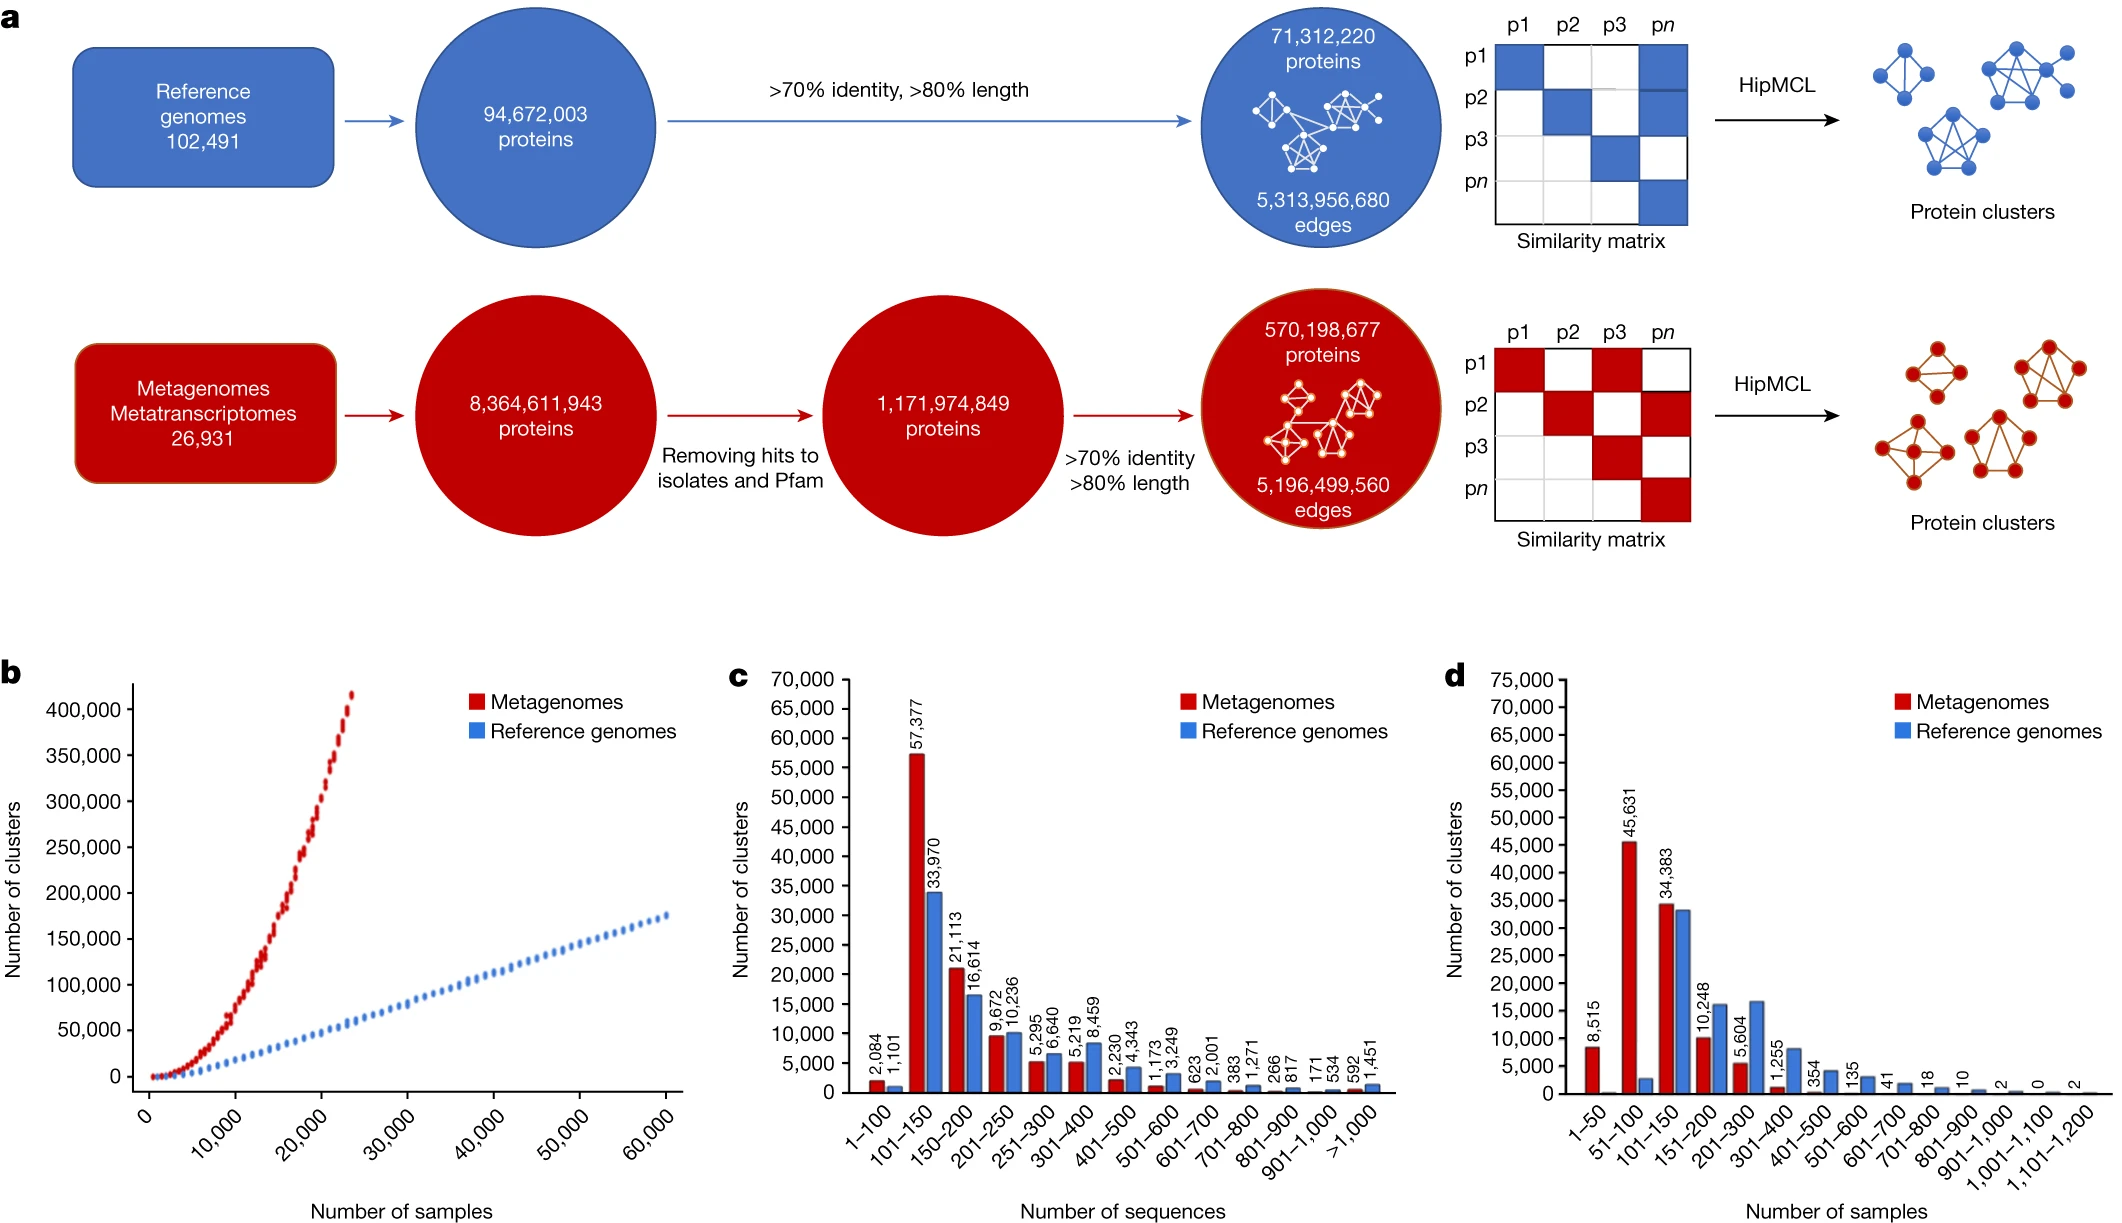
\includegraphics[width=1\linewidth]{asset/darkmatter.png}
  \caption{Overview of large-scale protein clustering from \cite{darkMatter}.
  (a) Pipeline: reference genomes (102k) and metagenomes (26k) yield billions
  of protein sequences. Pairwise similarities are filtered using thresholds of
  \(\geq\)70\% sequence identity and \(\geq\)80\% alignment coverage, producing
  sparse graphs with hundreds of millions of nodes and billions of non-trivial
  edges, which are clustered using HipMCL. (b) As new samples are added to the
  input dataset (Number of samples), this shows how many clusters appear in the
  graph cumulatively (Number of clusters). Only the clusters with at least 100
  sequences per cluster are included. (c) Cluster size distribution:
  heavy-tailed, with many small clusters and few large ones. (d)
  Cluster distribution across samples: most clusters are restricted to a small
  number of samples, while few are widely distributed. These results
  collectively highlight the scale, extreme sparsity, and structural
  heterogeneity of protein sequence similarity networks.}
  \label{fig:darkMatter}
\end{figure}
% b. Incrementally recompute pipeline after expanding the input dataset. Why rectangles instead of points for each N number of samples? Perhaps, for each sample size they re-computed the pipeline for multiple collection of N samples. The latter is not excplicitly clarified in the paper however rarefaction plots usually involve random sampling to supress bias.

From a computational perspective, large-scale sequence clustering naturally
leads to graph-based formulations. Protein sequences can be represented as
nodes in a graph, with edges encoding similarity relationships derived from
pairwise sequence alignment scores. Community detection algorithms can then be
applied to identify densely linked subgraphs corresponding to putative protein
families or functional groups. While this formulation is conceptually
straightforward, its practical implementation at scale poses significant computational challenges.

As demonstrated by \cite{ssn}, sequence similarity networks offer a scalable
and interpretable framework for visualizing relationships across large protein
superfamilies. For example, human GPCRs (G protein‑coupled receptors), a
diverse family of membrane proteins involved in cellular signaling. Overlaying
such networks with orthogonal information, such as taxonomic classification
or functional annotation, reveals functional themes and highlights outliers,
making them a powerful tool for exploratory analysis. Unlike phylogenetic
trees or multiple sequence alignments, networks can accommodate far larger
datasets while preserving both global structure and local details. An example
is shown in Fig.~\ref{fig:ssn1}.

\begin{figure}[htbp]
  \centering
  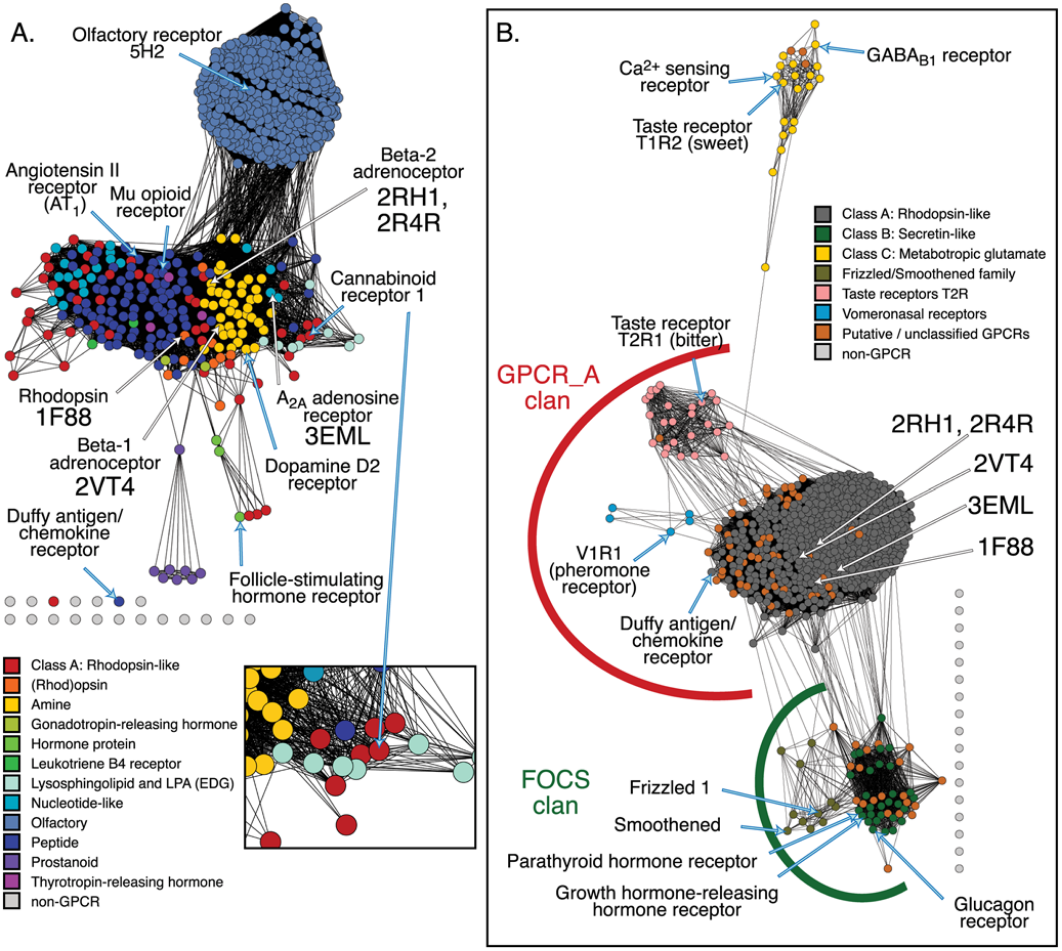
\includegraphics[width=0.9\linewidth]{asset/ssn1.png}
  \caption{Sequence similarity networks of human kinase domains from
  \cite{ssn}. Nodes represent proteins; edges indicate significant sequence
  similarity. (A) Network colored by kinase class, revealing functional
  groupings. (B) Network colored by the presence of a catalytic lysine in the
  VAIK motif, showing how orthogonal information can be overlaid to identify
  sequence features. This illustrates how sequence similarity networks can
  visualize relationships across large protein families (513 sequences) and
  overlay orthogonal information.}
  \label{fig:ssn1}
\end{figure}

\subsection*{Scope and Contribution of Current Work}

The goal of this thesis is to investigate the practical scalability of
community detection methods for protein sequence networks. Rather than
proposing new algorithms, an existing workflow is adopted and its execution is
carefully streamlined and tailored to evaluate the performance of community
detection algorithms under various configurations. Using large protein
sequence datasets derived from reference proteomes, PSSNs are constructed and
clustered using established tools, including MCL and HipMCL executed on a
single compute node.

This work is guided by three core priorities:

\begin{enumerate}
  \item \textbf{Scalability}: Establishing the practical limits of MCL and
    HipMCL on a single compute node.
  \item \textbf{Reproducibility}: Ensuring the entire workflow is
    portable, well‑documented, and executable with publicly available
    tools.
  \item \textbf{Interpretability}: Using graph‑based representations and
    alignment‑derived similarity, which provide direct biological meaning
    without black‑box embeddings.
\end{enumerate}

The primary emphasis of this study is on computational performance with limited
emphasis on the evaluation of the results. Precise biological validation of the
resulting clusters is considered outside the main scope of this work. Instead,
the focus is placed on the computational challenges that arise when applying
widely used clustering algorithms to large biological datasets on a single
compute node, and on identifying practical limitations encountered in this
environment.

By systematically documenting these observations, this thesis aims to assess
the capabilities and limitations of reproducible and interpretable community
detection applied to sparse PSSNs comprising millions of vertices representing
protein sequences. Such an assessment is intended to inform both computational
scientists developing scalable algorithms and bioinformaticians seeking to
apply these methods to large biological datasets in practical computing
environments.

  \cleardoublepage
  \section{Background}
\chead{\thesection. Background}

\subsection{The Central Dogma of Molecular Biology}

The central dogma of molecular biology defines the directional flow of genetic
information within a living system. This framework was first articulated by
Francis Crick in 1958 and has since been supported by decades of experimental
evidence \cite{centralDogma}. Crick's formulation distinguished three
sequential transfers that occur in all cellular organisms: DNA to DNA,
DNA to RNA, and RNA to protein. He also noted that other transfers, such as
protein to DNA, do not occur in nature.

Deoxyribonucleic acid (DNA) serves as the primary hereditary macromolecule. A
segment of DNA that encodes a functional product, such as a protein or
functional RNA, is defined as a \textit{gene}. The information stored in a gene
is first copied into messenger RNA (mRNA) in a process called
\textit{transcription}. The mRNA macromolecule is then decoded to assemble a
linear chain of amino acids, a protein, through \textit{translation}. This
directional flow is summarised as:

\[
\text{DNA} \xrightarrow{\text{transcription}} \text{mRNA} \xrightarrow{\text{translation}} \text{Protein}.
\]

The structure of these linear macromolecules is composed of residue monomers
(observe Fig.~\ref{fig:central_dogma} and
Appendix~\ref{appendix:aminoAcidLookup}). The central dogma ends at the primary
structure of a protein --- the linear sequence of amino acid residues. This
sequence determines the protein's higher-order structure and function, but
those properties are not directly encoded in the DNA. For computational protein
analysis, the primary structure is the central object of study, as
it can be directly compared across species and used to infer evolutionary and
functional relationships as well as the protein's spatial structure.

\begin{figure}[htbp]
  \centering
  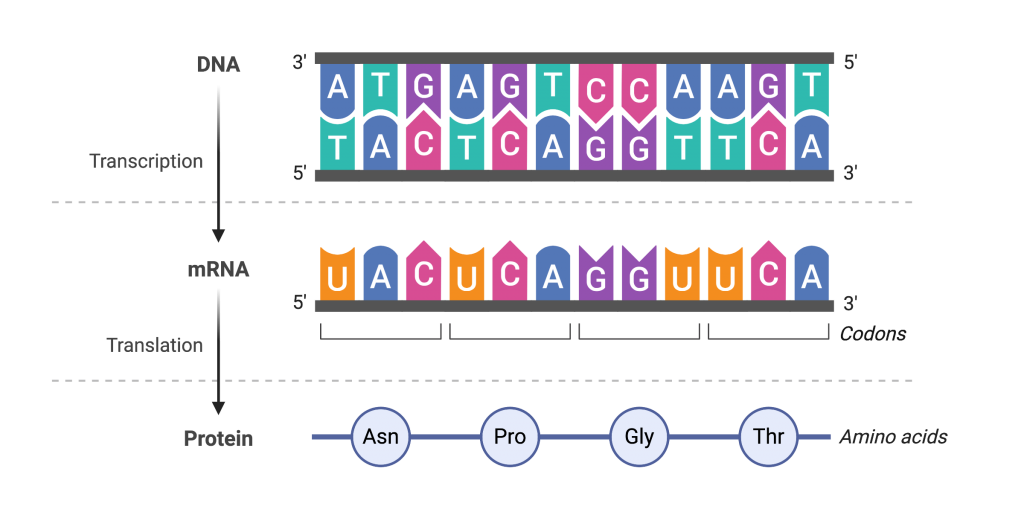
\includegraphics[width=1\linewidth]{asset/central_dogma.png}
  \caption{Flow of genetic information in a cellular organism. This image was created with BioRender (\href{https://www.biorender.com}{biorender.com}).}
  \label{fig:central_dogma}
\end{figure}

Proteins with similar sequences often share evolutionary origin or function ---
in the sense that they descend from a common ancestor, much like species in the
\textit{tree of life}. Grouping proteins by sequence similarity is therefore a
fundamental task in bioinformatics. This problem naturally maps to community
detection on weighted graphs where each protein becomes a vertex, edges connect
similar proteins, and clusters correspond to protein families.

\subsection{The Markov Cluster Algorithm}
\label{subsec:mcl}

MCL is a community detection algorithm that receives as input a weighted graph
and produces a set of communities (vertex clusters) by simulating a random
walk~\cite{mcl}. It is deterministic with respect to its input, therefore the
initial graph conditions yield a reproducible collection of output clusters.
Additionally, the algorithm is mathematically polished and well
studied~\cite{mclDetailed} while its algorithmic simplicity gives room
for computational optimization and scalability. For instance, the
implementation of HipMCL~\cite{hipmcl}, a high performance computing (HPC)
variant of MCL, is able to reliably process huge graphs comprised of at
least \(10^8\) vertices given that the compute cluster is sufficiently large.
MCL is capable of producing high quality clustering with a relatively low
computational cost and little need for tuning compared to other protein
clustering models. These properties collectively make MCL a suitable baseline
model for the task of biological sequence clustering, with a long track record
in a diverse set of tasks in biological sequence analyses~\cite{mclBrohee,
mclVlasblom, mclHaue, mclGibbons}.

Below is an algorithmic construction of MCL, applied on protein sequence data.
The purpose of this formulation is to provide a foundation, primarily for understanding
the computational complexity and memory requirements of the algorithm, which
are central to evaluating its scalability. At the same time, the formulation
highlights the stochastic mechanisms underlying MCL. We begin with a set of
definitions that establish the necessary groundwork.

\textbf{Definition 1}. For some \(n \in \mathbb{N}^*\), a \textit{weighted graph} is defined as \((\mathscr{V}, \mathcal{A})\), where \(\mathscr{V} = \{ v_i : i \in \{ 1, \dots, n \} \}\) holds all the graph's vertices and \(\mathcal{A}: \{ 1, \dots, n \}^2 \rightarrow \mathbb{R}\) is a square matrix where each row \(j\) and column \(k\) corresponds to vertices \(v_j\) and \(v_k\) respectively. The \(\mathcal{A}_{j,k}\) element of \(\mathcal{A}\) is the directed weight from the column \(k\) vertex to the row \(j\) vertex. \(\mathcal{A}\) is called the \textit{adjacency matrix}, and its elements satisfy the property
\[
  \forall j,k \in \{ 1, \dots, n \} \left( \mathcal{A}_{j, k} \geq 0 \ \wedge \ \mathcal{A}_{j, j} = 1 \right).
\]

\textbf{Definition 2}. For a weighted graph \((\mathscr{V}, \mathcal{A})\), if the adjacency matrix satisfies \(\mathcal{A}_{j, k} = \mathcal{A}_{k, j}\), then each element's weight is directionless, and \((\mathscr{V}, \mathcal{A})\) is called an \textit{undirected graph}.

\textbf{Definition 3}. For a weighted undirected graph \((\mathscr{V}, \mathcal{A})\), if \(\mathscr{V}\) is comprised of protein sequences and \(\mathcal{A}_{j,k}\) models the pairwise similarity of \(v_j, v_k \in \mathscr{V} \ ( j,k \in \mathbb{N}^* )\), then \((\mathscr{V}, \mathcal{A})\) is called a \textit{Protein Sequence Similarity Network} (\textit{PSSN}).

\textbf{Definition 4}. For a weighted graph \((\mathscr{V}, \mathcal{A})\), the \textit{Markov matrix} \(\mathcal{M}\) is a square matrix \(\mathcal{M}: \{ 1, \dots, n \}^2 \rightarrow [0, 1]\) where the value of cell \(\mathcal{M}_{j, k}\) semantically expresses the conditional \textit{probability of transition} from vertex \(v_k\) to \(v_j\) at the initial state with index $0$. Hence, \(\mathcal{M}_{j,k}\) acts as \(\mathcal{P}(v_j \ | \ v_k, \ \tau=0)\) in probabilistic literature.

\textbf{Remark}. In this case, the graph represents a stochastic system, where the \(k\) column of \(\mathcal{M}\) is normalized with respect to the \(k\) column of \(\mathcal{A}\) (observe Eq.~\ref{eq:markovMat}). Hence, the vector
\[
  \mathcal{M}_{\cdot, k} =
  \begin{pmatrix}
    \mathcal{P}(v_q \ | \ v_k, \ \tau=0) : q \in \{ 1, \dots, n \}
  \end{pmatrix}
\]
is a discrete probability distribution (PD).

For some set of protein sequences \(\mathscr{V}\), suppose that there exists a
pairwise similarity measure of that set's elements. Specifically, assume that
for each pair \(v_j, v_k \in \mathscr{V}\) there is some non-negative number
\(\mathcal{A}_{j,k} > 0\) encoding the pair's evolutionary similarity.
In the latter case, the adjacency
matrix \(\mathcal{A}\) quantifies a pairwise homology score between the
proteins \(v_k\) and \(v_j\) for all \(j, k \in \{ 1, \dots, n \}\). A
homologous protein collection descends from a common ancestral gene, and is
assumed to differ due to mutations, transcriptional\footnote{In genomics,
transcription is the process through which DNA generates the initial form of
RNA.} errors, or other sources of protein-sequence divergence.  On that basis,
the graph \((\mathscr{V}, \mathcal{A})\) is a PSSN representing the stochastic
system's initial state conditions at \textit{time} or \textit{step} \(\tau =
0\), and the task is to group together homologous proteins.

For proper usage of MCL and to preserve numerical stability throughout the internal iterations of the underlying random walk, \(\mathcal{A}\) must first be subjected to column-wise normalization. Thus, for every \(j,k \in \{ 1, \dots, n \}\), we set
\begin{align}
  \mathcal{M}_{j, k} := \dfrac{\mathcal{A}_{j, k}}{\sum_{q=1}^{n} \mathcal{A}_{q, k}}.
  \label{eq:markovMat}
\end{align}
Considering the fact that \(\mathcal{M} : \{ 1, \dots, n \}^2 \rightarrow [0, 1] \) is column normalized, each column represents a discrete PD, which in conjunction with the graph's independence from past states, implies that \(\mathcal{M}\) is a Markov matrix. Since each column of \(\mathcal{M}\) is a PD, its
\begin{align}
  \sum_{q=1}^{n} \mathcal{M}_{q, k} = 1
  \label{eq:sum1}
\end{align}
for all \(k \in \{ 1, \dots, n \}\).

The element \(\mathcal{M}_{j, k}\) is a measure of tendency for the vertex
\(v_k\) to land onto the vertex \(v_j\) after exactly one transition and can
thus be interpreted as the conditional probability \(\mathcal{P}(v_j \ | \ v_k,
\ \tau = 0)\). This tendency displays a directed \textit{flow of information} in
the graph. Also, because the measure is semantically tied to the protein pair's
evolutionary similarity, higher values express a higher statistical certainty
that the protein pair is homologous.
Subsequently, zero elements of \(\mathcal{M}\) correspond to disallowed vertex
transitions, representing non-homologous sequence pairs.

It is worth mentioning that \(\mathcal{A}\)'s symmetry does not ensure
\(\mathcal{M}\)'s symmetry because of the column-wise normalization performed
in Eq.~\ref{eq:markovMat}. The transition to the next state of the graph
depends entirely on its present state, making it independent from all previous
states. This is called the Markovian property of the stochastic system. This
property significantly simplifies the stochastic evolution of the graph towards
the next states, giving room for more interpretable and computationally
tractable approaches to the problem of protein clustering, while eliminating
the overhead of a more complicated mathematical structure and unnecessary
computational complexity.

Now we are ready to construct MCL in an iterative
form that underlies the aforementioned random walk. The integer \(\lambda \in
\mathbb{N}^*\) will denote the index of a specific random walk iteration.
Within that iteration, the stochastic system undergoes at least one state
transition --- through a parameter \(e\) which will be specified later. At
iteration \(\lambda\), MCL performs a transformation to some matrix
\(\mathcal{M}^{(\lambda-1)}\) called the \textit{transition matrix}. This
transformation produces another updated transition matrix\footnote{The notation
of the transition matrix \(\mathcal{M}^{(\lambda)}\) differs from
\(\mathcal{M}^{\lambda}\). In the former notation, the symbol \((\lambda)\)
wrapped in parentheses, represents a superscript, while in the latter the
integer \(\lambda\) represents an exponent of the Markov matrix
\(\mathcal{M}\).} \(\mathcal{M}^{(\lambda)}\).

This update simulates \textit{flow} in the graph, effectively pushing up the
probability of transition for sequence pairs with high correlation, while
decreasing that probability for pairs with low correlation. Given a sufficient
number of repetitions, the compounding effect of this repeated process on the
\(\mathcal{M}\) matrix eventually captures the strongest protein sequence edges
of similar proteins, and as a consequence, tightly connected proteins are
categorized into a collection of disjoint sub-regions that are called
communities or graph clusters (observe section 5 of \cite{mclDetailed}).

This process is outlined in the following pseudocode snippet:
\begin{plaintext}[showspaces=false, literate=]
Set parameters $e$ and $r$.
$\lambda := 1$
$\mathcal{M}^{(0)} := \mathcal{M}$
{
   $\texttt{w} := \mathcal{E}_e \mathcal{M}^{(\lambda-1)} \hspace*{0.00cm}$ # Expand.
   $\texttt{w} := \mathcal{Q} \texttt{w}                  \hspace*{1.121cm}$ # Prune.
   $\texttt{w} := \Gamma_r \texttt{w}                     \hspace*{1.044cm}$ # Inflate.
   $\mathcal{M}^{(\lambda)} := $ w
   $\lambda := \lambda + 1$
} Repeat while $\mathcal{M}^{(\lambda)}$ changes significantly compared to $\mathcal{M}^{(\lambda-1)}$.
\end{plaintext}

All details of the latter loop condition, as well as the operations of expansion \(\mathcal{E}_e\), pruning \(\mathcal{Q}\) and inflation \(\Gamma_r\) are detailed below. To complete the initialization of the iterative process, first set \(\lambda := 1\) and \(\mathcal{M}^{(0)}:=\mathcal{M}\).

\subsubsection{Expansion}

Expansion \(\mathcal{E}_e\) is an operator that subjects the probability matrix \(\mathcal{M}^{(\lambda)}\) to multi-step transitions in a single MCL iteration. Its parameter
\[
  e \ : \ e \in \mathbb{N} \ ( e \geq 2 )
\]
represents the number of state transitions applied per iteration. Say from iteration with index \(\lambda\) to \(\lambda+1\), the operation \(\mathcal{E}_e\) effectively expands the random walk's length, by incrementing the number of graph states by \(e-1\). Therefore, we have that
\begin{align}
  \mathcal{E}_e(\mathcal{M}^{(\lambda)}) = (\mathcal{M}^{(\lambda)})^e.
  \label{eq:expansion}
\end{align}
Since \(\mathcal{M}^{(\lambda)}\) is the transition matrix of the graph at iteration \(\lambda\), the statement
\begin{align}
  \mathcal{M}^{(\lambda)}_{j,k} = \mathcal{P}(v_j \ | \ v_k, \ \tau = (e-1) \cdot \lambda) 
  \label{eq:expProb}
\end{align}
holds for all \(j,k \in \{ 1, \dots, n \}\).

For lower exponent values \(e\), information propagates more smoothly in the graph after each subsequent MCL iteration. Hence, for \(e=2\) the transition matrix avoids supressing potentially valuable structural information before inflation can act.
In the official MCL implementation\footnote{\url{https://github.com/micans/mcl}.}, the value of the exponent \(e\) is set to \(2\). This is an appropriate choice in a computational setting since this setup prevents overshooting convergent solutions.

In this case, for any \(j,k \in \{ 1, \dots, n \}\), it's
\begin{align*}
  \mathcal{E}_{\epsilon}(\mathcal{M}^{(\lambda)})
  & \overset{(\ref{eq:expansion})}{=} \left(\left( \mathcal{M}^{(\lambda)} \right)^2\right)_{j, k}
  \\
  & = \sum_{q = 1}^{n} ( \mathcal{M}^{(\lambda)}_{j, q} \cdot \mathcal{M}^{(\lambda)}_{q, k} )
  \\
  & \overset{(\ref{eq:expProb})}{=} \sum_{q = 1}^{n} \left( \mathcal{P}(v_j \ | \ v_q, \ \tau = \lambda) \cdot \mathcal{P}(v_q \ | \ v_k, \ \tau = \lambda) \right). 
\end{align*}
Notice that expansion does not break the probabilities of \(\mathcal{M}^e\), since all elements of \(\mathcal{M}^e\) belong to the interval \([0, 1]\), and each matrix column sums to 1 (observe Appendix~\ref{appendix:proofExp}).

To preserve the output, we assign it in \texttt{w}, i.e., \(w := \mathcal{E}_e \mathcal{M}^{(\lambda)}\).

\subsubsection{Pruning}

After the expansion of the transition matrix \(\mathcal{M}^{(\lambda)}\), it is expected for many elements of the output matrix \texttt{w} to be extremely small.
These near-zero elements behave effectively like zero with negligible contribution to the dynamics of the random walk. On the other hand, sparsity is a desirable property that lowers the computational cost during subsequent iterations.
Thus, to increase graph sparsity and further leverage its computational benefit, all smaller value elements may be discarded based on an appropriate dynamic threshold \(f_k\) as a function of column index \(k\).

Since each column (node) carries its own PD per column \(\texttt{w}_{\cdot,k}\) with index \(k \in \{ 1, \dots, n \}\), the range of each column is unique and thus the threshold should be computed based on the statistical descriptors of the column's PD.
To respect this constraint, one way to model pruning is by first defining some constants \(a \in (0, 1]\) and \(b \in \{ 1, \dots, 8 \}\). Then set
\begin{align}
  f_k = a \cdot \text{ctr}(\texttt{w}_{\cdot, k}) \cdot \Big( \ 1 - b \cdot \big( \max( \texttt{w}_{\cdot, k} ) - \text{ctr}(\texttt{w}_{\cdot, k}) \big) \ \Big)
  \label{eq:pruningThreshold}
\end{align}
where
\[
  \text{ctr}(\texttt{w}_{\cdot, k}) = \Bigg( \sum_{j = 1}^{n} \texttt{w}_{j, k}^2 \Bigg)^{\frac{1}{2}}.
\]
Thus for a column \(k\), first compute the threshold \(f_k\) based on Eq.~\ref{eq:pruningThreshold}, and then for each row \(j\), if \( \texttt{w}_{j, k} < f_k \) is true then the element \( \texttt{w}_{j, k} \) is considered as trivial and through \textit{pruning} it gets discarded, i.e., \( \texttt{w}_{j, k} := 0 \).

\subsubsection{Inflation}

The role of inflation is to amplify edges that link node pairs belonging within a cluster (intra-cluster edges), while suppressing edges between nodes that belong to two different clusters (inter-cluster edges).
This happens through a straightforward element-wise exponentiation of the matrix \( \texttt{w} \), to the power of some parameter \( r \in \mathbb{R} \ (r > 1) \). Namely,
\[
  \Gamma_r \texttt{w} = ( \texttt{w}_{j, k}^{r} : j, k \in \{ 1, \dots, n \} ).
\]
Since MCL determines the number of clusters internally, it is important for the designer to have some control over that number. A way to control that number is by overriding the inflation parameter \(r\).
The selection of the exponent parameter \(r\) has an indirect influence on the \textit{granularity} of the final clusters. Granularity is a property of how fine grained the resulting clusters are, collectively. More specifically,
\begin{itemize}
  \item \(r \uparrow\) implies finer granularity : By increasing \(r\), we expect finer grained cluster collection, hence a higher number of smaller clusters.
  \item \(r \downarrow\) implies coarser granularity : By decreasing \(r\), we expect coarser grained cluster collection, hence a lower number of larger clusters.
\end{itemize}
Usually, the selection \(r\) is bounded in the interval \([1.2, 5]\).

Generally, inflation provides a simple yet effective tuning mechanism for exploring the network's community structure at different resolutions.

\subsubsection[Stochasticity Reconstruction \& \ Termination Condition]{Stochasticity Reconstruction \& Termination Condition}

Matrix \(\texttt{w}\) is not necessarily a transition matrix given the aforementioned transformations that it was subjected to.
This is a problem if we want to continue applying these transformations iteratively since at this point, \(\texttt{w}\) has lost the probabilistic structure that conveys the weighted graph's flow.
That is why, as a final step of iteration \(\lambda\), the matrix \(\texttt{w}\) is converted into a transition matrix through the following normalization. Thus, we now set the updated transition matrix as
\begin{align*}
  \mathcal{M}^{(\lambda+1)}_{j,k} := \texttt{w}_{j,k} \Big{/} \sum_{q=1}^{n} \texttt{w}_{q,k}
\end{align*}
for all \(j,k \in \{ 1, \dots, n \}\).

This entire process is practically repeated up to some finite iteration \(\lambda_0\), in which the update from \(\mathcal{M}^{(\lambda_0-1)}\) to \(\mathcal{M}^{(\lambda_0)}\) is insignificant with trivial changes on the latter stochastic matrix at \(\lambda_0\) compared to the preceding one at iteration \(\lambda_0-1\). The termination condition that defines \(\lambda_0\) could be implemented as follows
\begin{align}
  \left\| \mathcal{M}^{(\lambda)} - \mathcal{M}^{(\lambda-1)} \right\|_\text{F} < \epsilon_0 \cdot n^2
  \label{eq:term}
\end{align}
for some small enough value \(\epsilon_0 \in \mathbb{R} \ ( \epsilon_0 > 0)\), where \(\| \cdot \|_\text{F}\) is the Frobenius norm defined as
\[
  \left\| \mathcal{X} \right\|_\text{F} := \Bigg( \sum_{j=1}^{n} \sum_{k=1}^{n} \left| \mathcal{X}_{j,k} \right|^2 \Bigg)^{\frac{1}{2}}.
\]
In a computational setting, the loop of MCL will terminate when Eq.~\ref{eq:term} is satisfied for the first time.
According to the rigorous analysis performed in \cite{mclDetailed}, the
sequence \(\lambda \mapsto \mathcal{M}^{(\lambda)}\) can converge fast to some
block diagonal real matrix \(\lim_{\lambda \rightarrow \infty}
\mathcal{M}^{(\lambda)}\), given that the inflation parameter \(r\) is set to a
high enough value. The said matrix regions are tightly connected, typically
exhibiting a much higher sparsity compared to \(\mathcal{A}\). This result
allows us to safely assume the existence of some relatively low \(\lambda_0\)
that leads to a collection of clusters.

An example of an asymptotic transition matrix follows below:
\[
  \lim_{\lambda \rightarrow \infty} \mathcal{M}^{(\lambda)}
  \\
  =
  \begin{pmatrix}
0.34 & 0.32 & 0.33 & 0 & 0 & 0 & 0 & 0 & 0 & 0 & 0 & 0 \\
0.32 & 0.36 & 0.35 & 0 & 0 & 0 & 0 & 0 & 0 & 0 & 0 & 0 \\
0.33 & 0.32 & 0.32 & 0 & 0 & 0 & 0 & 0 & 0 & 0 & 0 & 0 \\
0 & 0 & 0 & 0.34 & 0.34 & 0.33 & 0.25 & 0 & 0 & 0 & 0 & 0 \\
0 & 0 & 0 & 0.34 & 0.37 & 0.32 & 0.26 & 0 & 0 & 0 & 0 & 0 \\
0 & 0 & 0 & 0.33 & 0.35 & 0.35 & 0.27 & 0 & 0 & 0 & 0 & 0 \\
0 & 0 & 0 & 0.25 & 0.21 & 0.32 & 0.32 & 0 & 0 & 0 & 0 & 0 \\
0 & 0 & 0 & 0 & 0 & 0 & 0 & 0.51 & 0.49 & 0 & 0 & 0 \\
0 & 0 & 0 & 0 & 0 & 0 & 0 & 0.48 & 0.52 & 0 & 0 & 0 \\
0 & 0 & 0 & 0 & 0 & 0 & 0 & 0 & 0 & 1 & 0 & 0 \\
0 & 0 & 0 & 0 & 0 & 0 & 0 & 0 & 0 & 0 & 0.53 & 0.47 \\
0 & 0 & 0 & 0 & 0 & 0 & 0 & 0 & 0 & 0 & 0.47 & 0.53
  \end{pmatrix}.
\]
In the example above, consider only the non-trivial blocks found in the
diagonal. Each such square submatrix represents an isolated region
corresponding to a distinct cluster. As it can be observed, there are five such
blocks in total. That is what the output of MCL may look like. Another example
can be observed in Fig.~\ref{fig:mcl_iter}, showcasing how MCL internally
processes an entangled graph starting from some complicated and relatively
sparse transition matrix \(\mathcal{M}\), until it successfully converges to a
disjoint collection of distinct regions without the initial noise of the weaker
edges.

\begin{figure}[htbp]

  \captionsetup[subfigure]{font=scriptsize}

  \vspace{-0.3cm}

  \hspace{0.5cm}
  \begin{subfigure}{0.40\linewidth}
    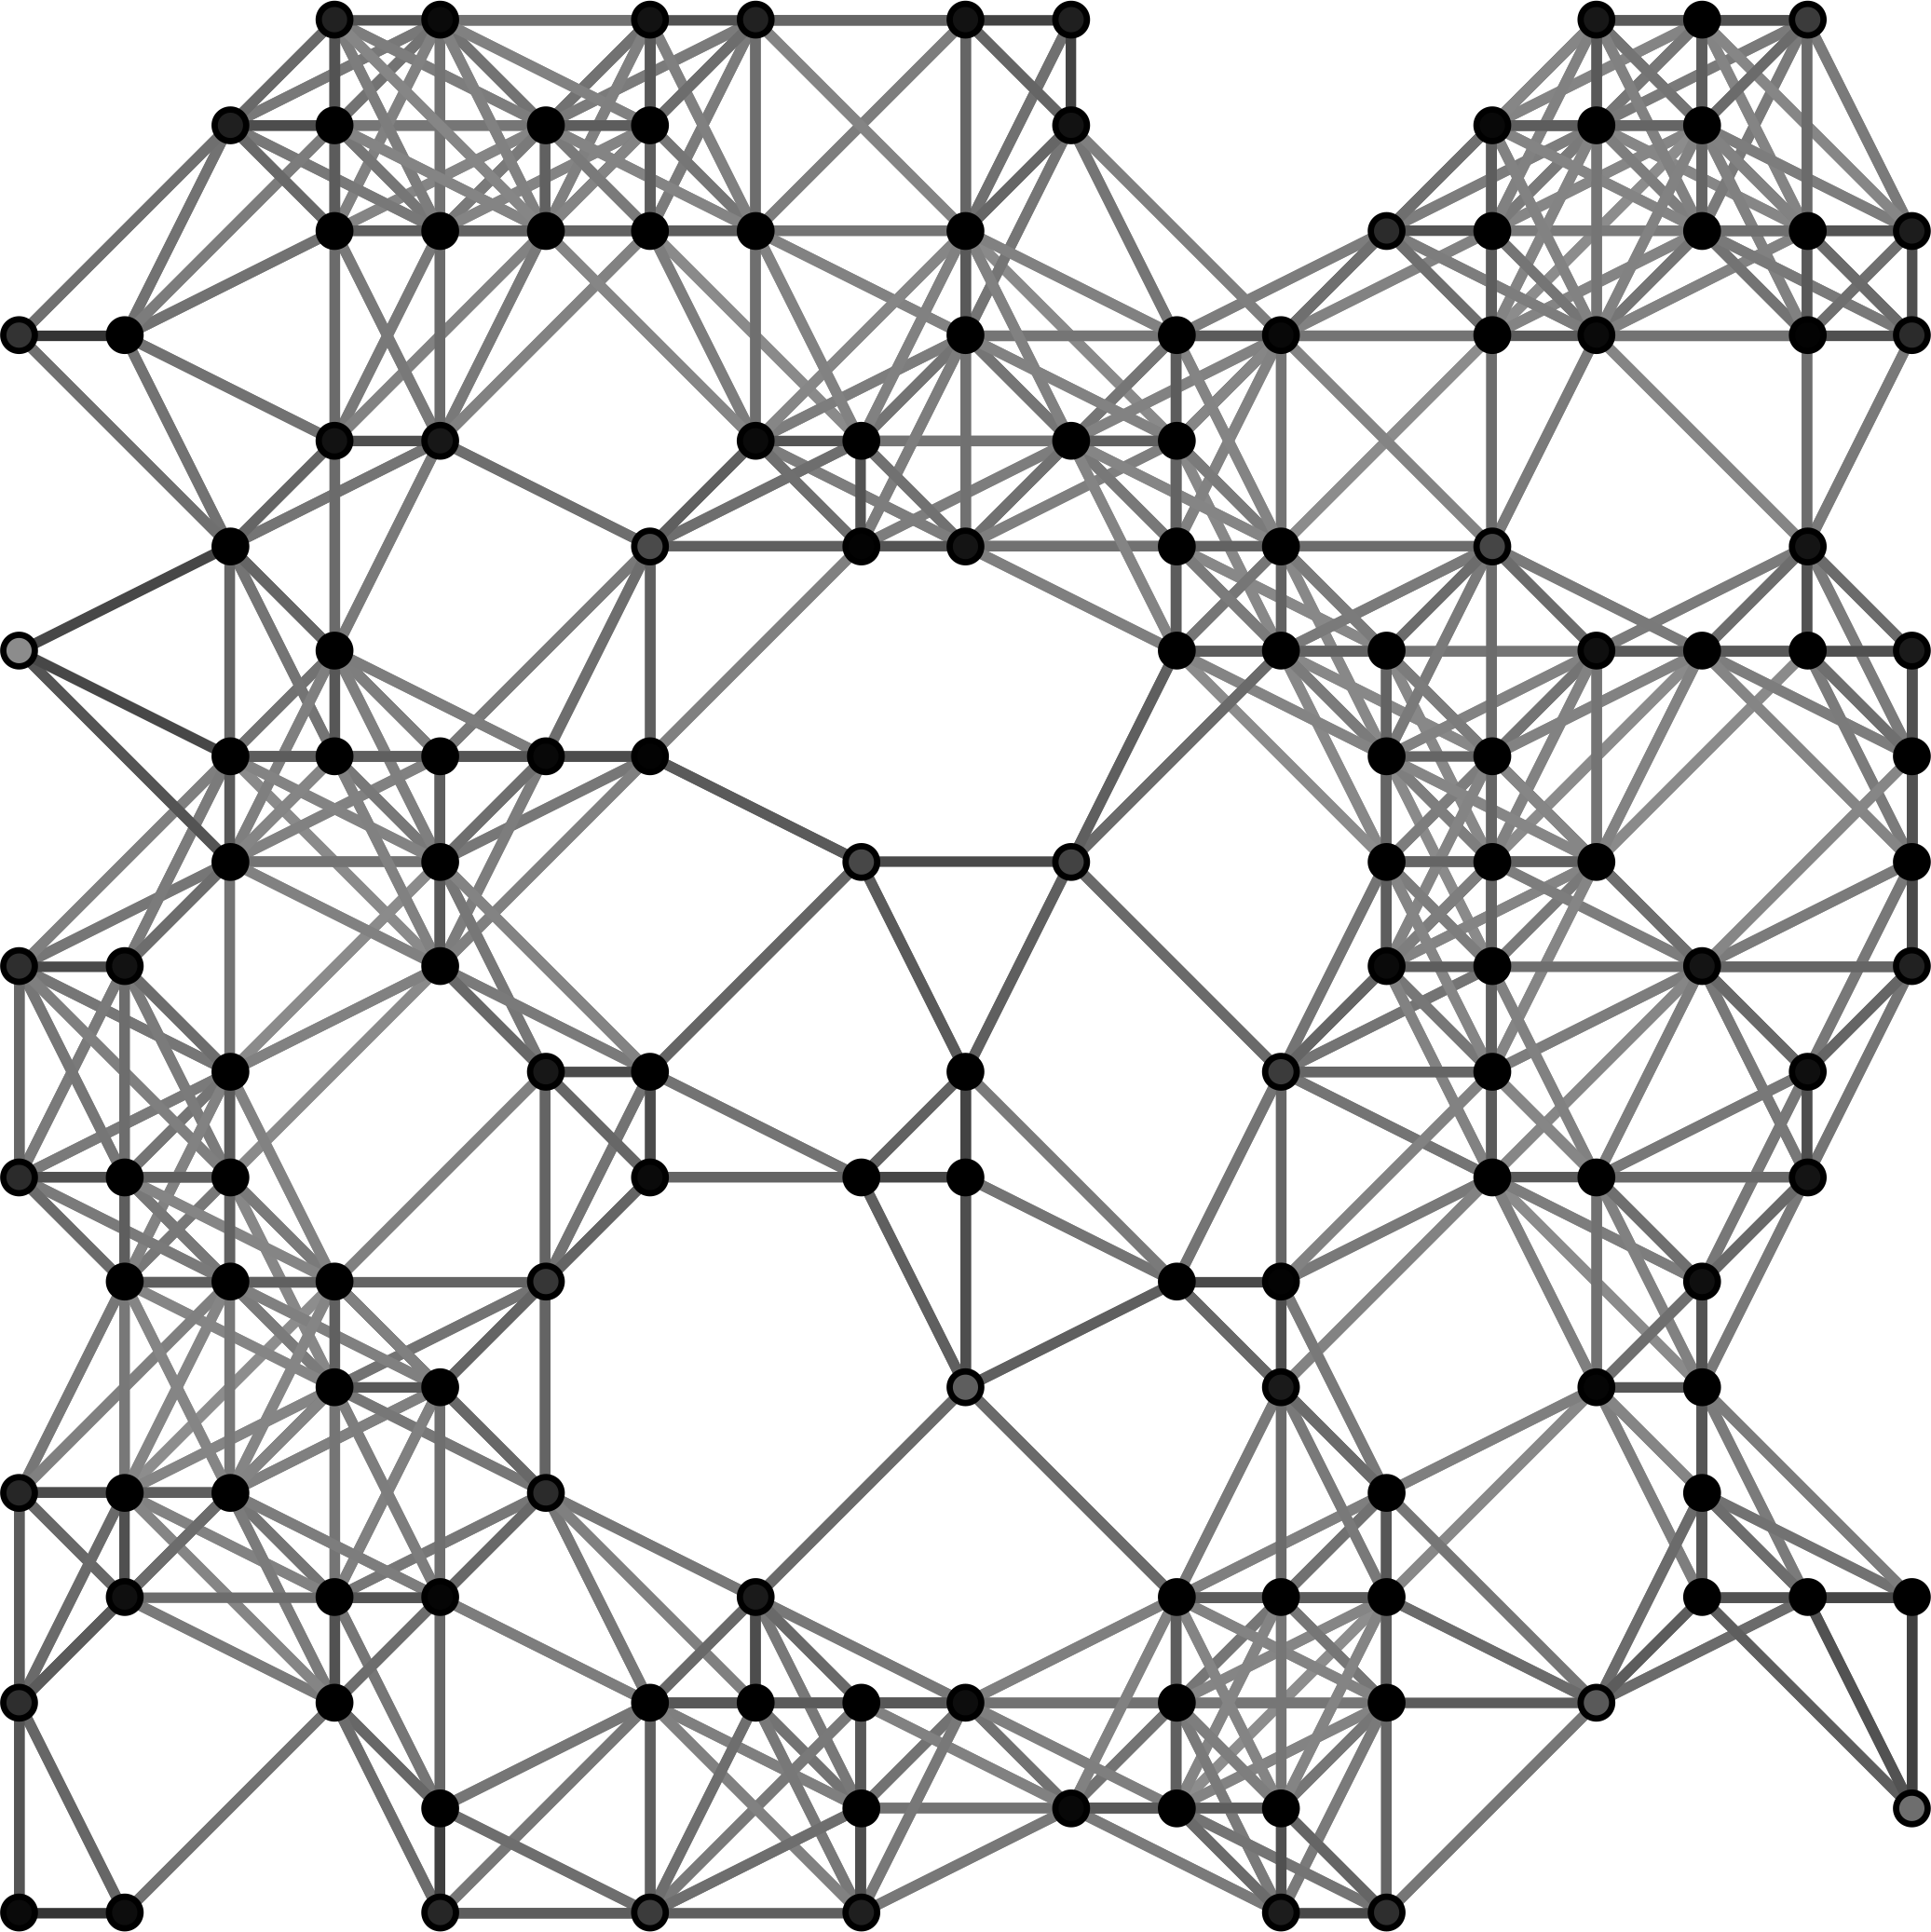
\includegraphics[width=\linewidth]{asset/mcl_iter_0.png}
    \subcaption{The pre-processed input graph \((\mathscr{V}, \mathcal{M})\) where \(\mathcal{M}\) is some sparse Markov matrix.}
    \label{fig:mcl_iter_1}
  \end{subfigure}
  \hfill
  \begin{subfigure}{0.40\linewidth}
    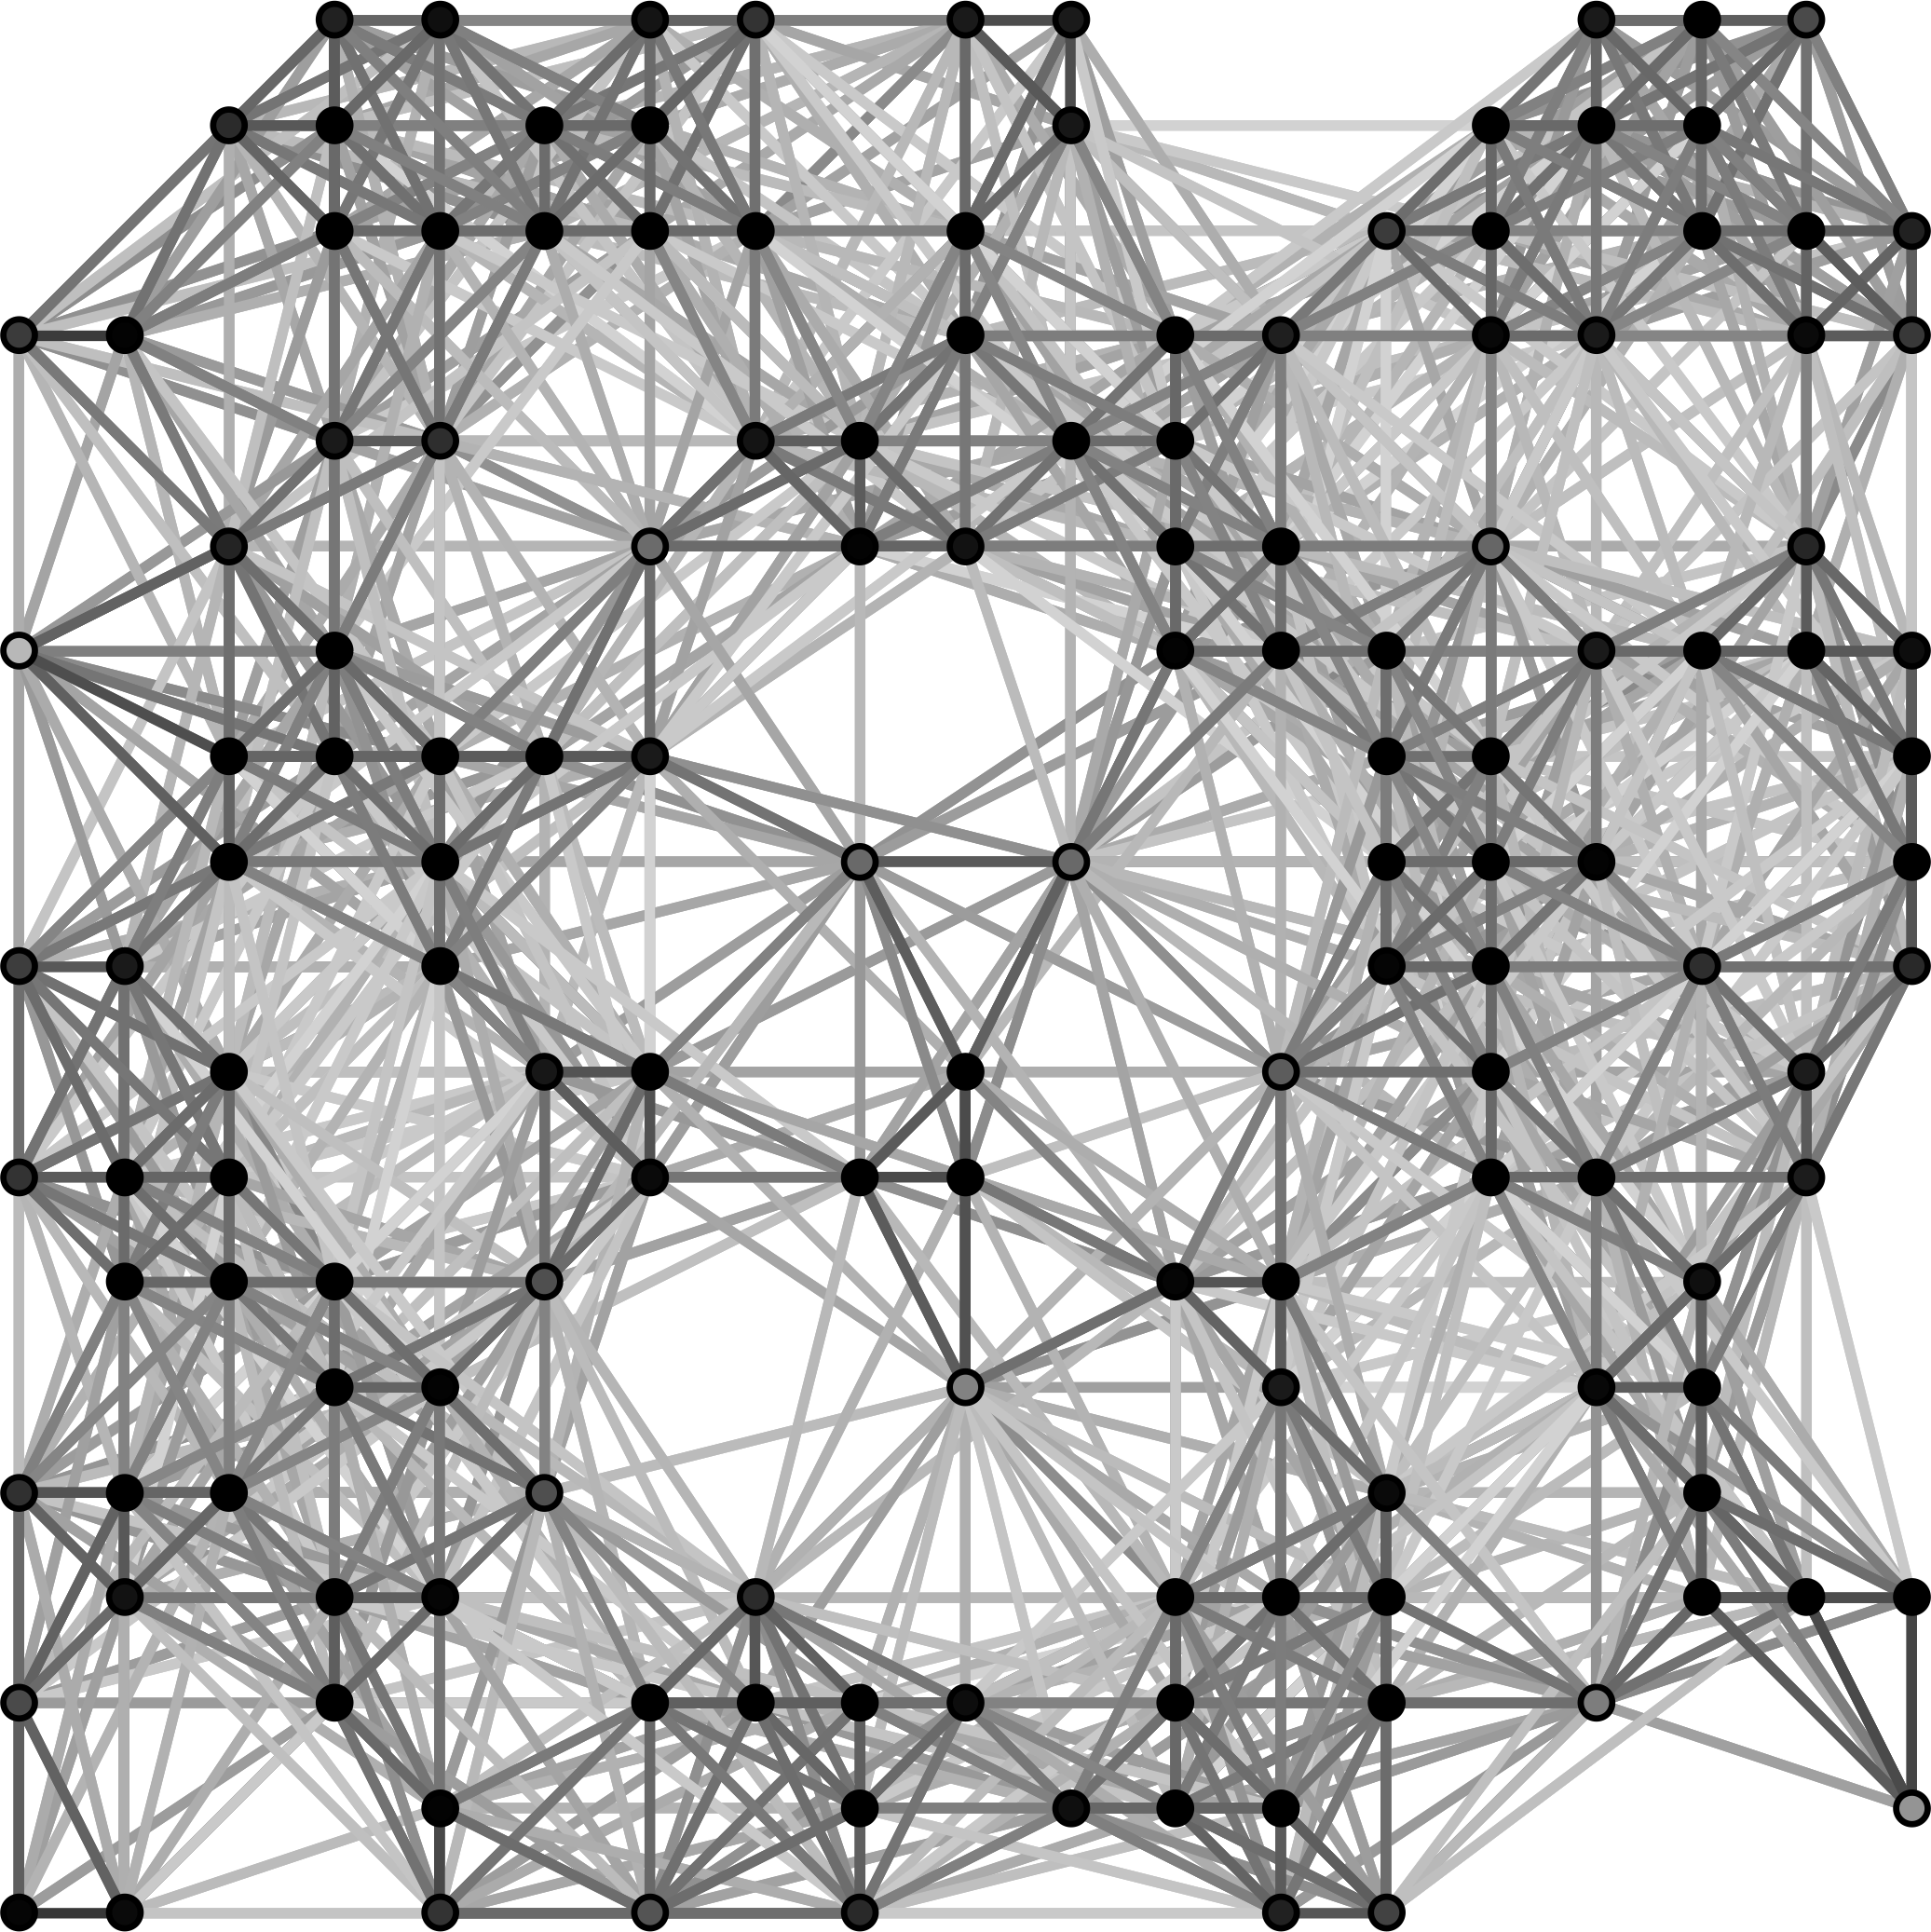
\includegraphics[width=\linewidth]{asset/mcl_iter_1.png}
    \subcaption{The graph with transition matrix \(\mathcal{M}^{(1)}\) after iteration 1.}
    \label{fig:mcl_iter_2}
  \end{subfigure}
  \hspace{0.5cm}

  \vspace{0.4cm}

  \hspace{0.5cm}
  \begin{subfigure}{0.40\linewidth}
    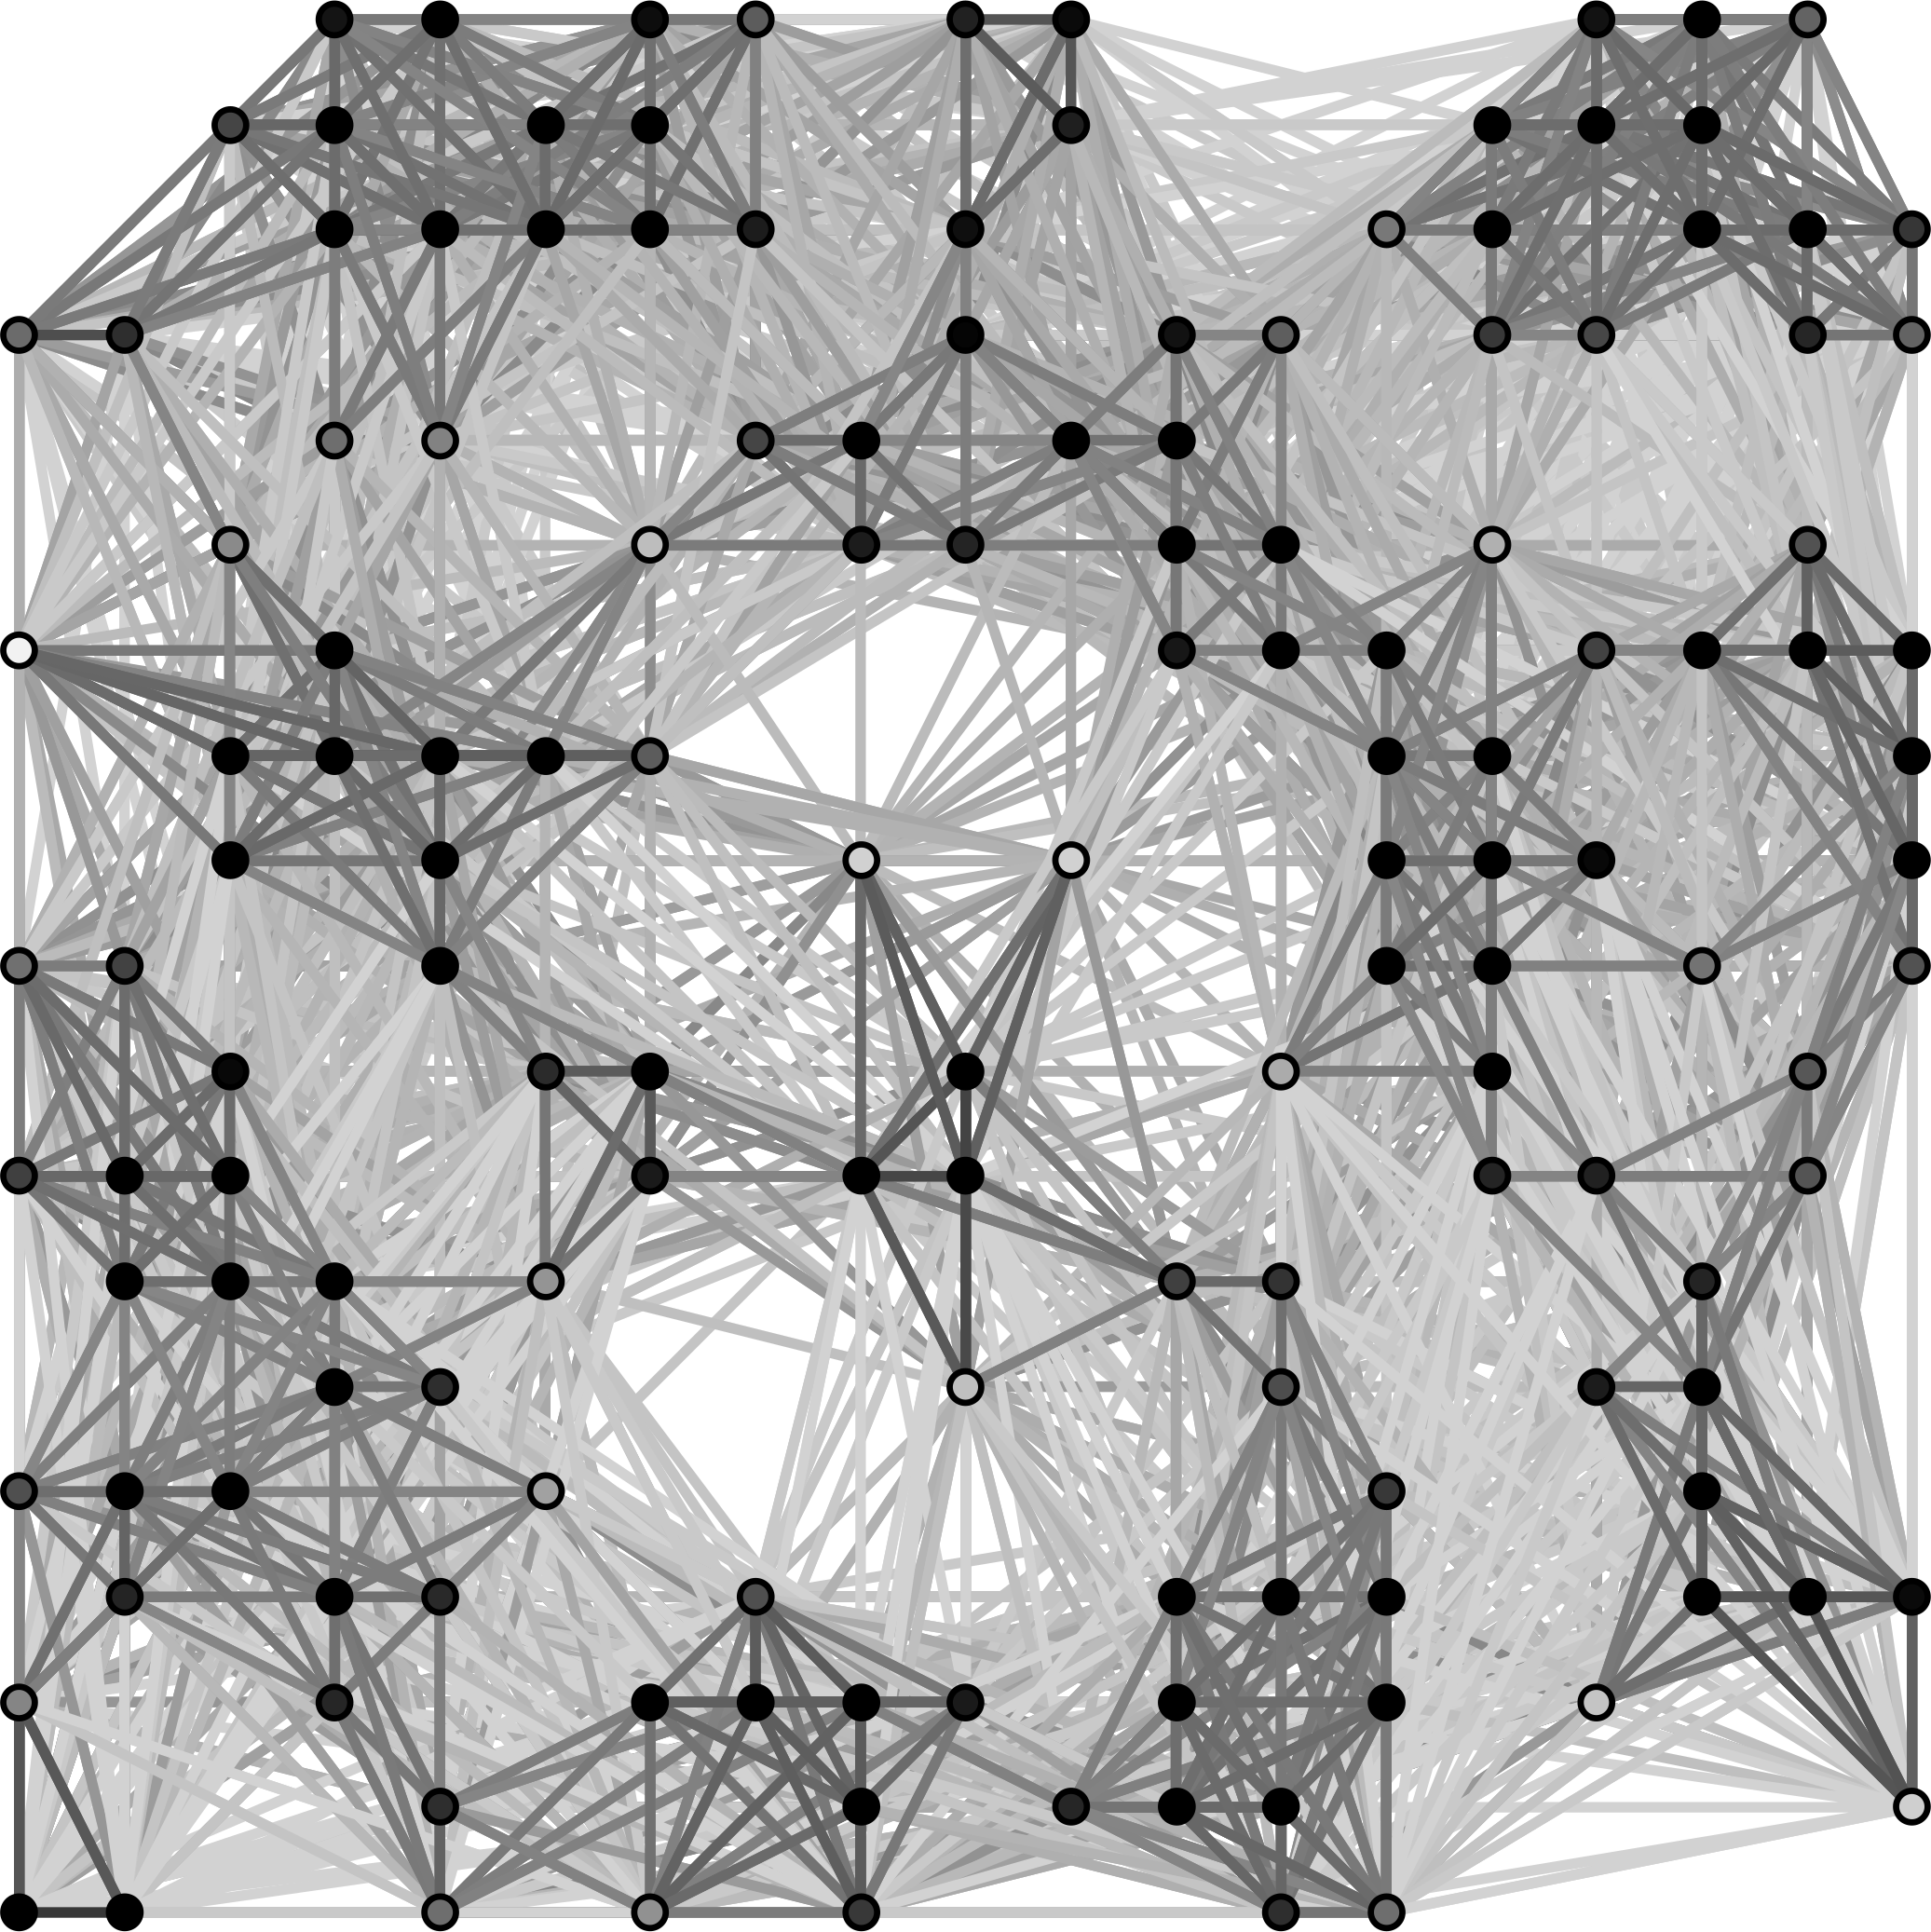
\includegraphics[width=\linewidth]{asset/mcl_iter_2.png}
    \subcaption{Transition matrix \(\mathcal{M}^{(2)}\) after iteration 2.}
    \label{fig:mcl_iter_3}
  \end{subfigure}
  \hfill
  \begin{subfigure}{0.40\linewidth}
    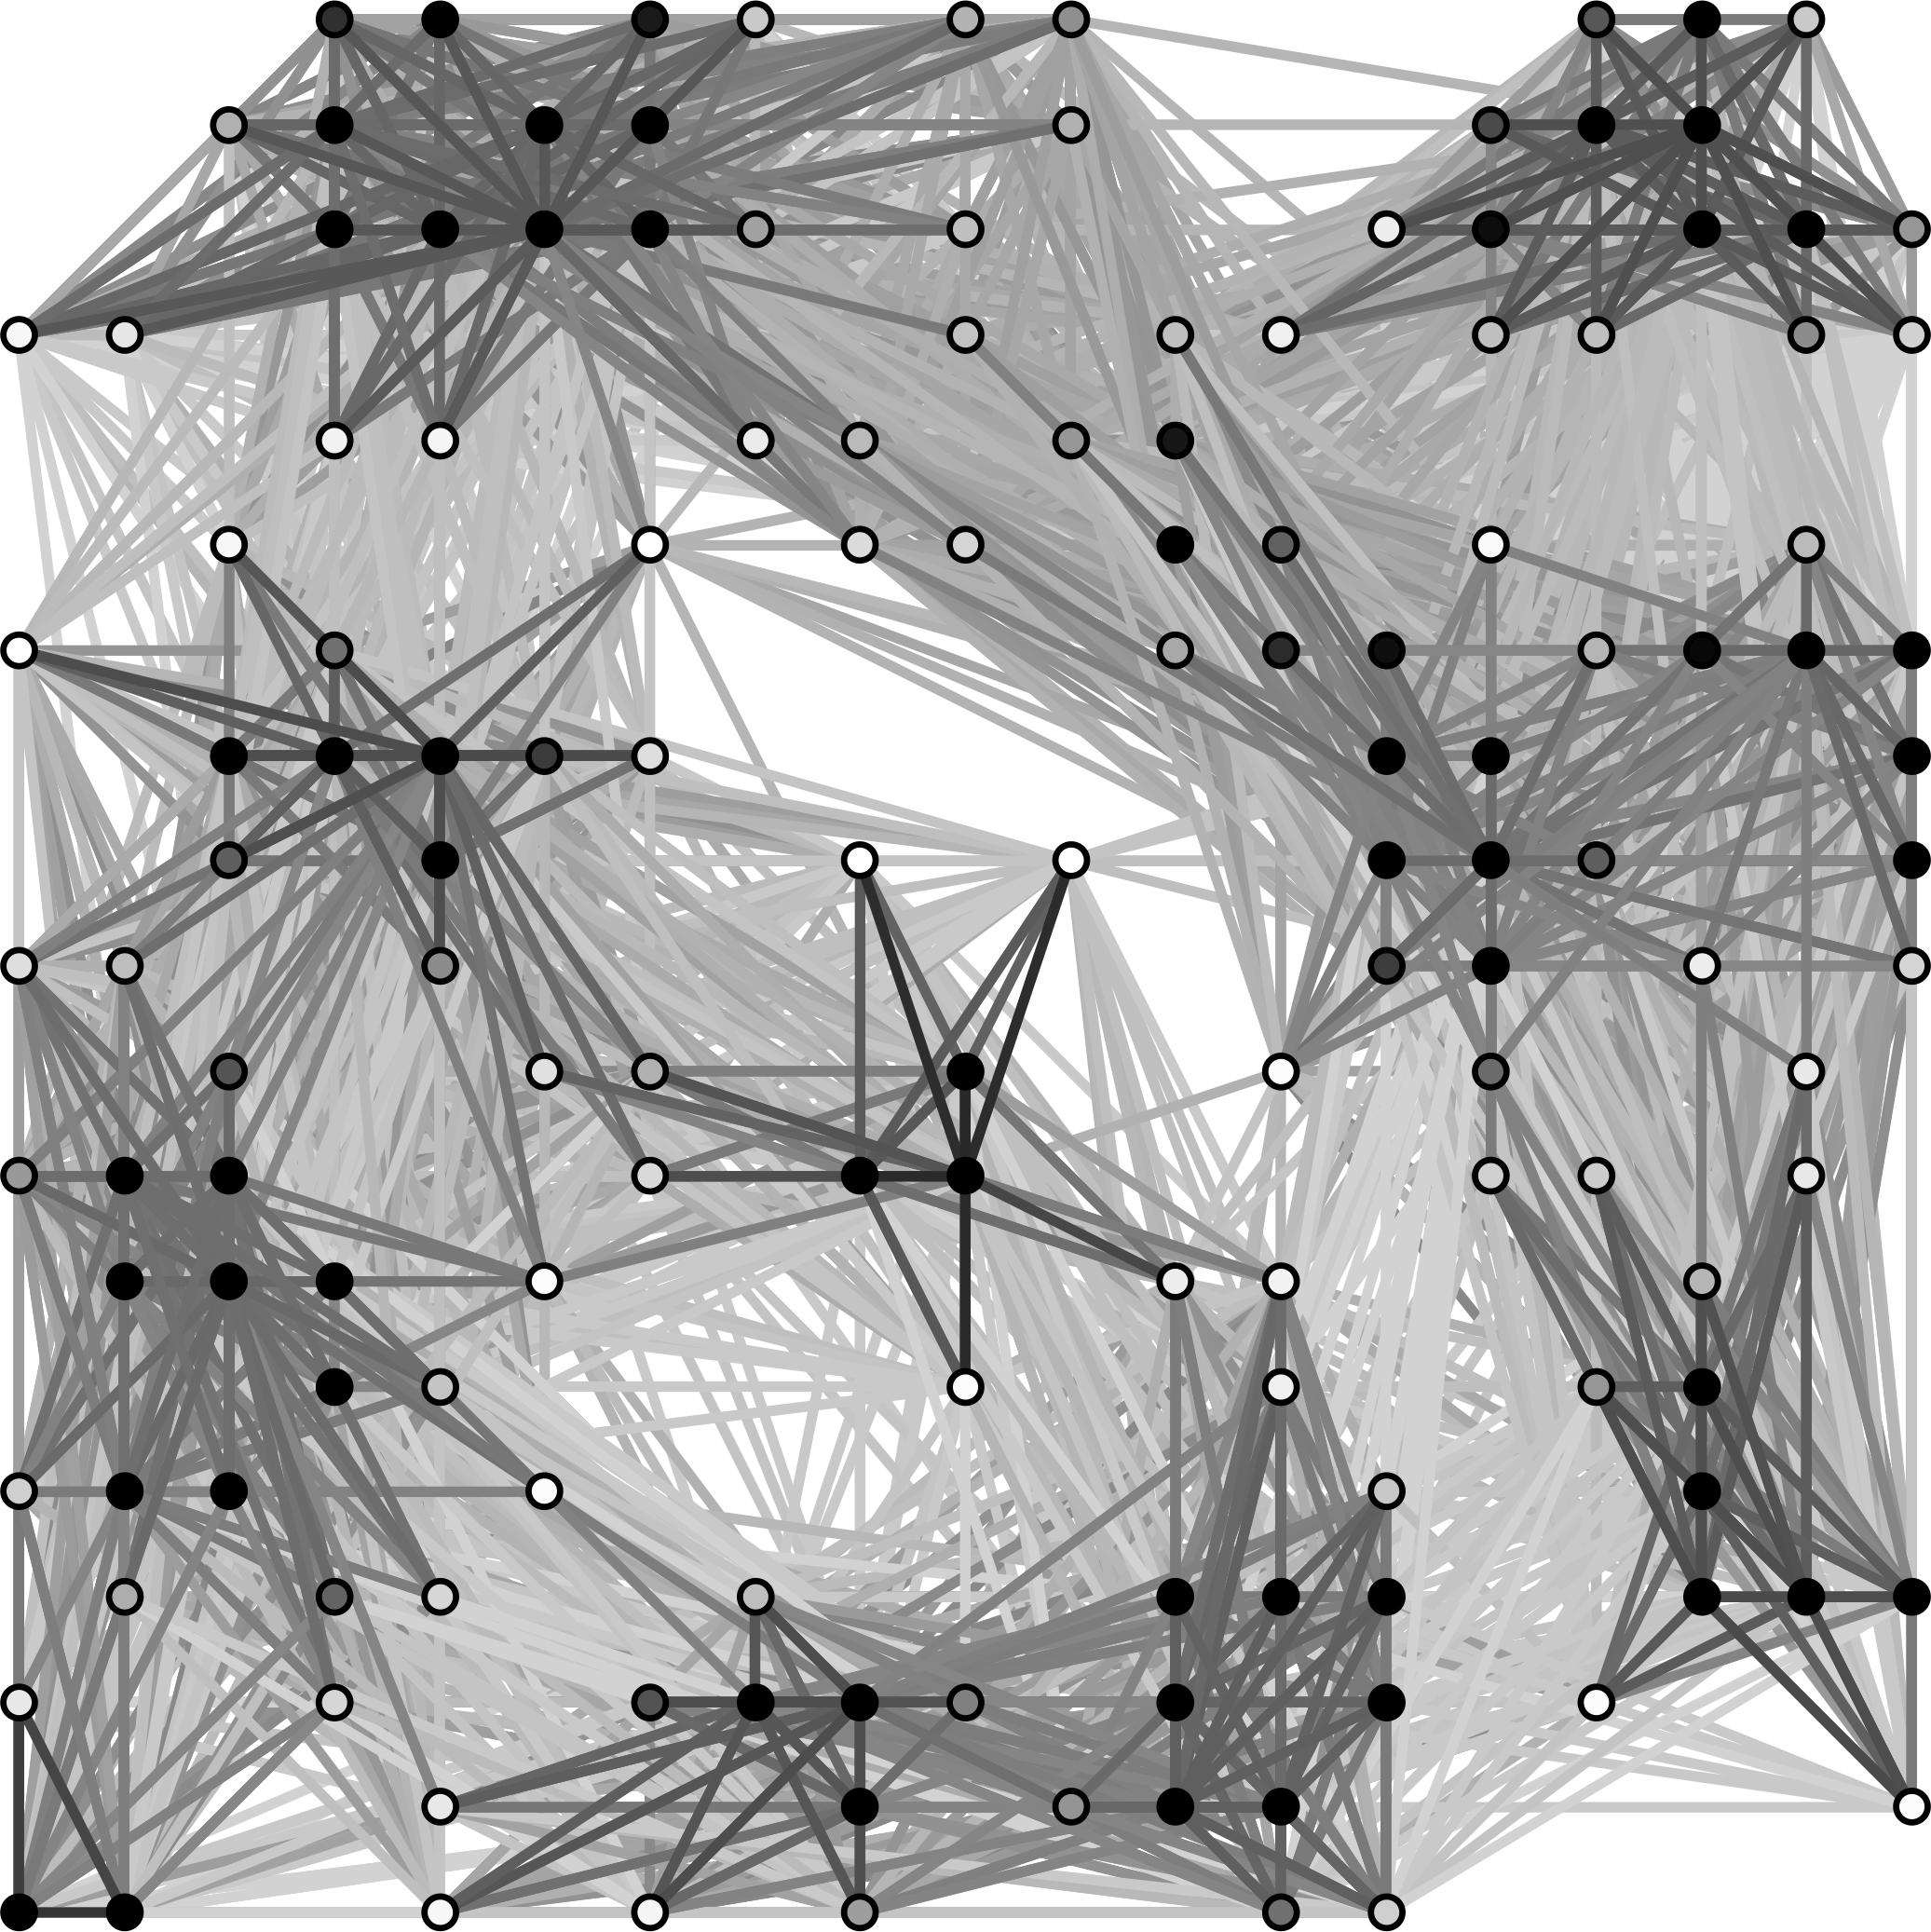
\includegraphics[width=\linewidth]{asset/mcl_iter_3.png}
    \subcaption{Transition matrix \(\mathcal{M}^{(3)}\) after iteration 3.}
    \label{fig:mcl_iter_4}
  \end{subfigure}
  \hspace{0.5cm}

  \vspace{0.4cm}

  \hspace{0.5cm}
  \begin{subfigure}{0.40\linewidth}
    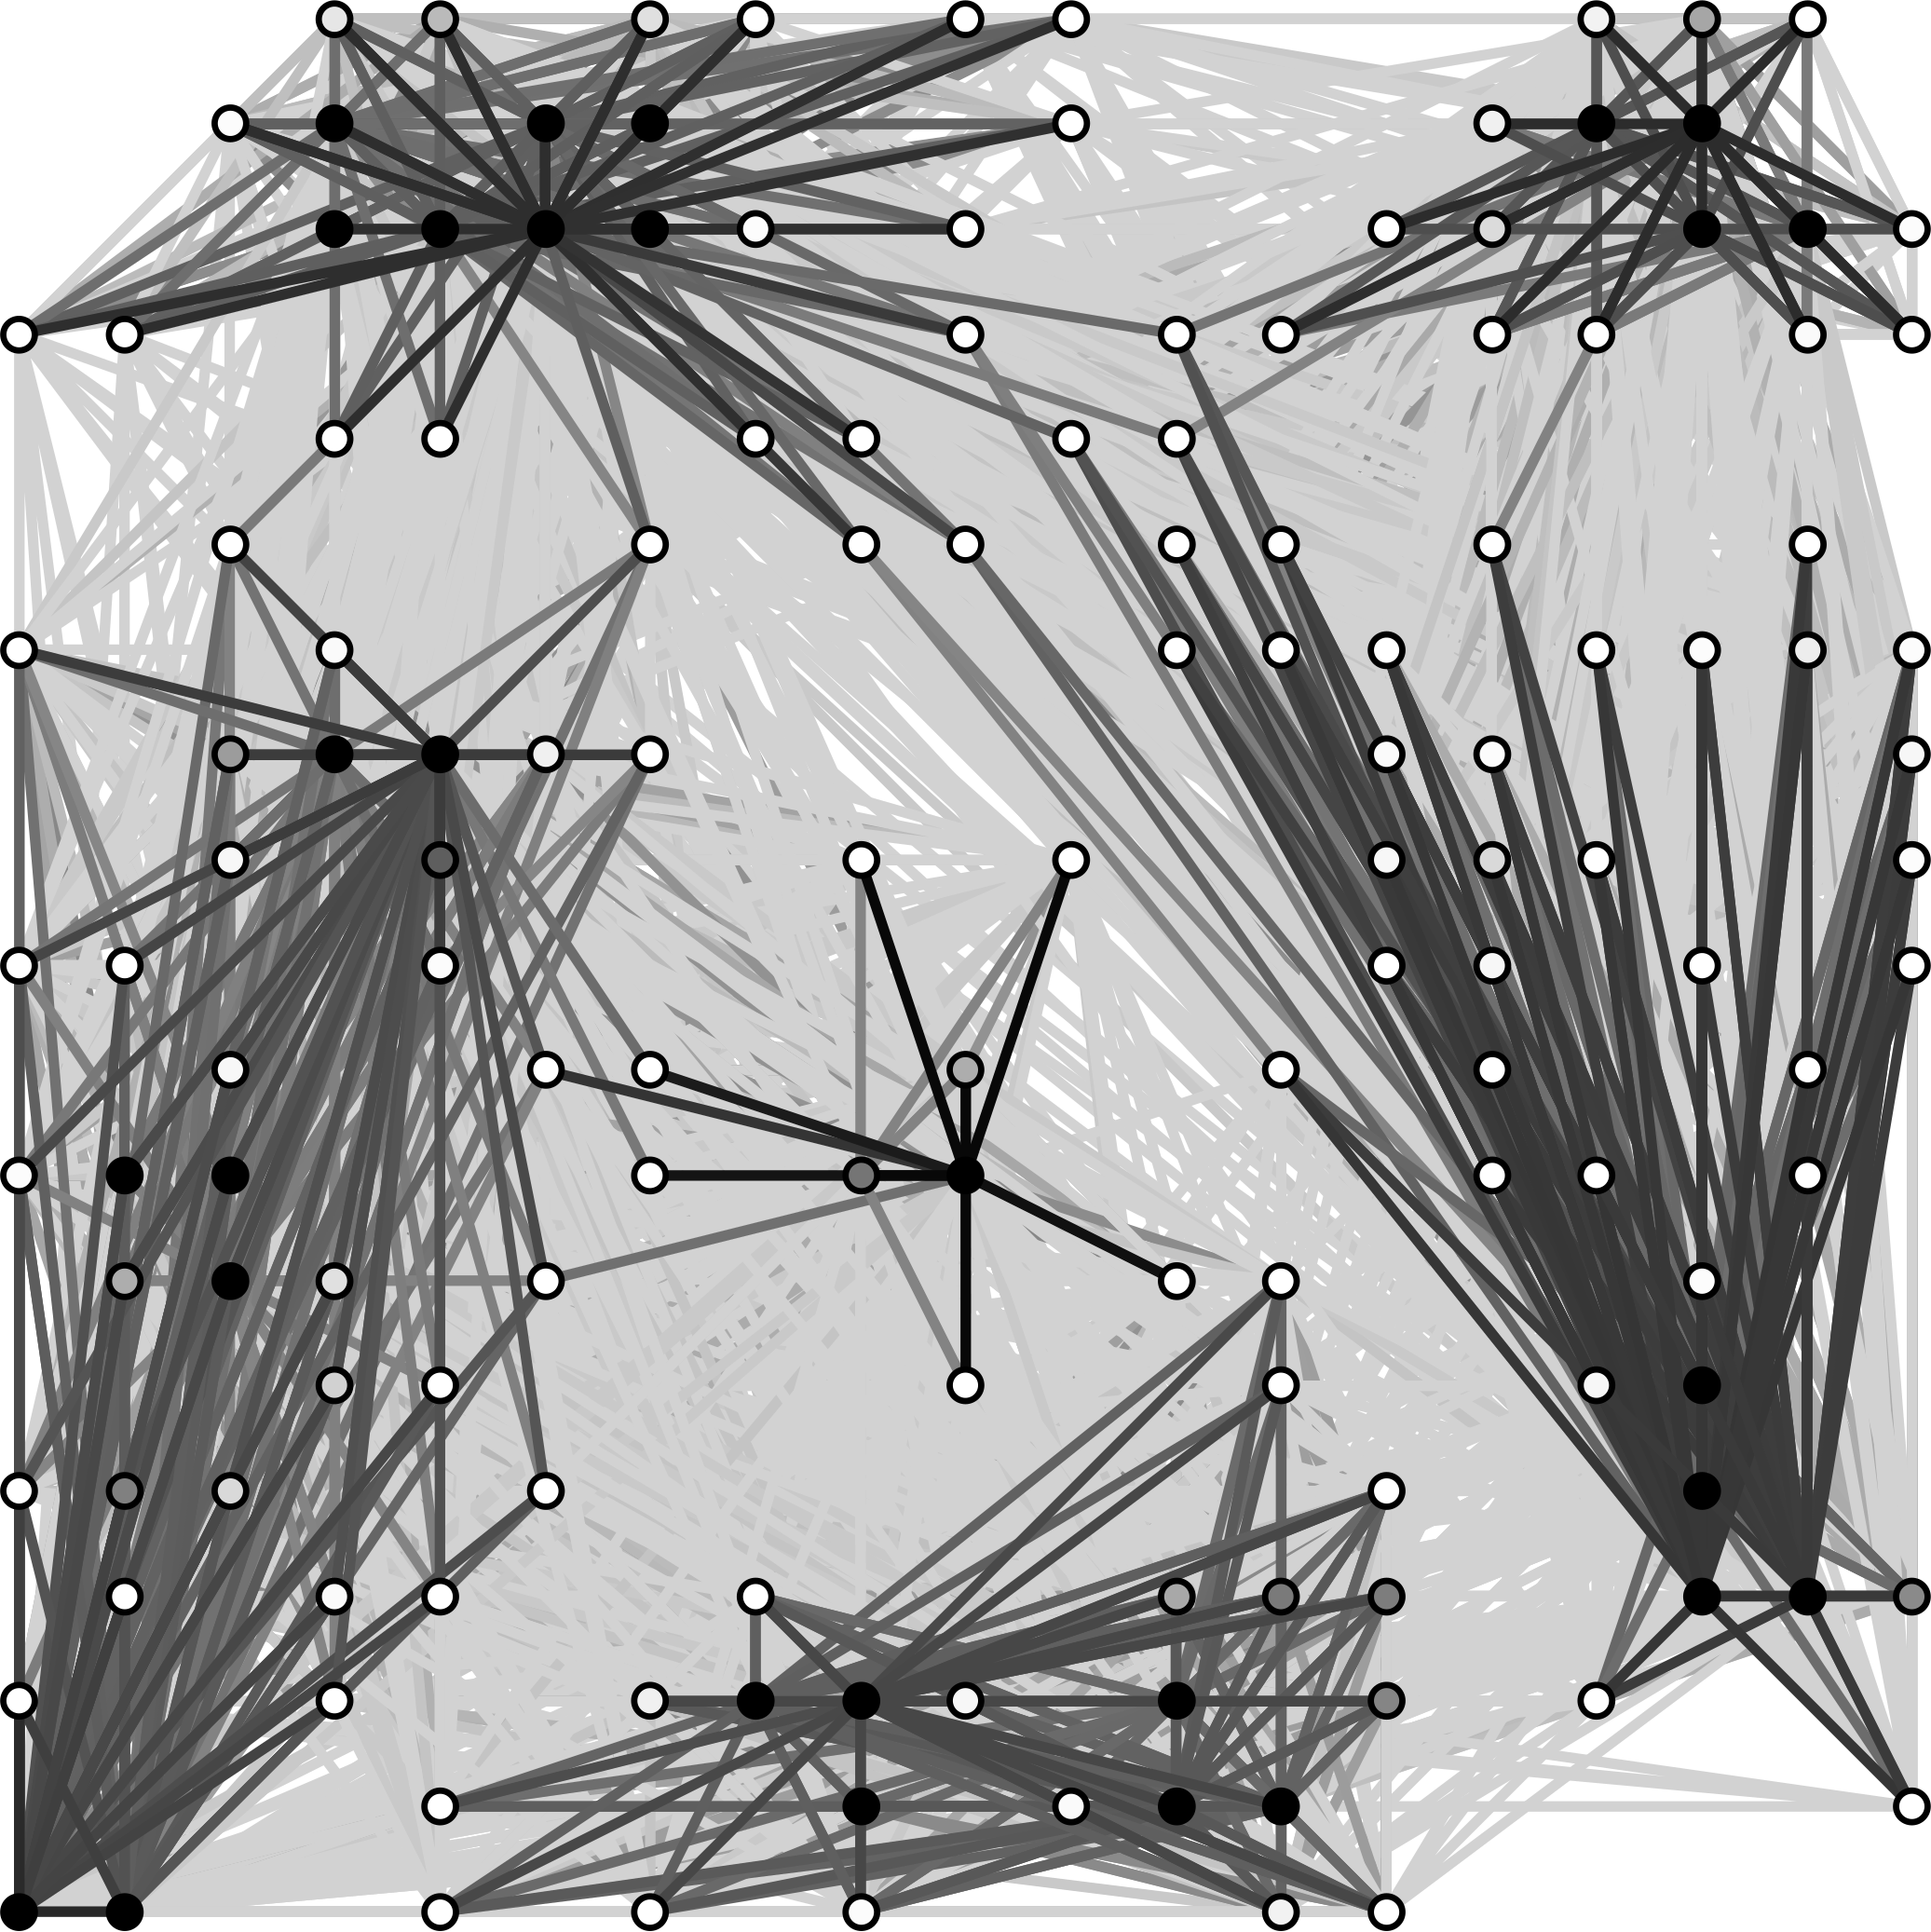
\includegraphics[width=\linewidth]{asset/mcl_iter_4.png}
    \subcaption{Transition matrix \(\mathcal{M}^{(4)}\) after iteration 4.\break}
    \label{fig:mcl_iter_5}
  \end{subfigure}
  \hfill
  \begin{subfigure}{0.40\linewidth}
    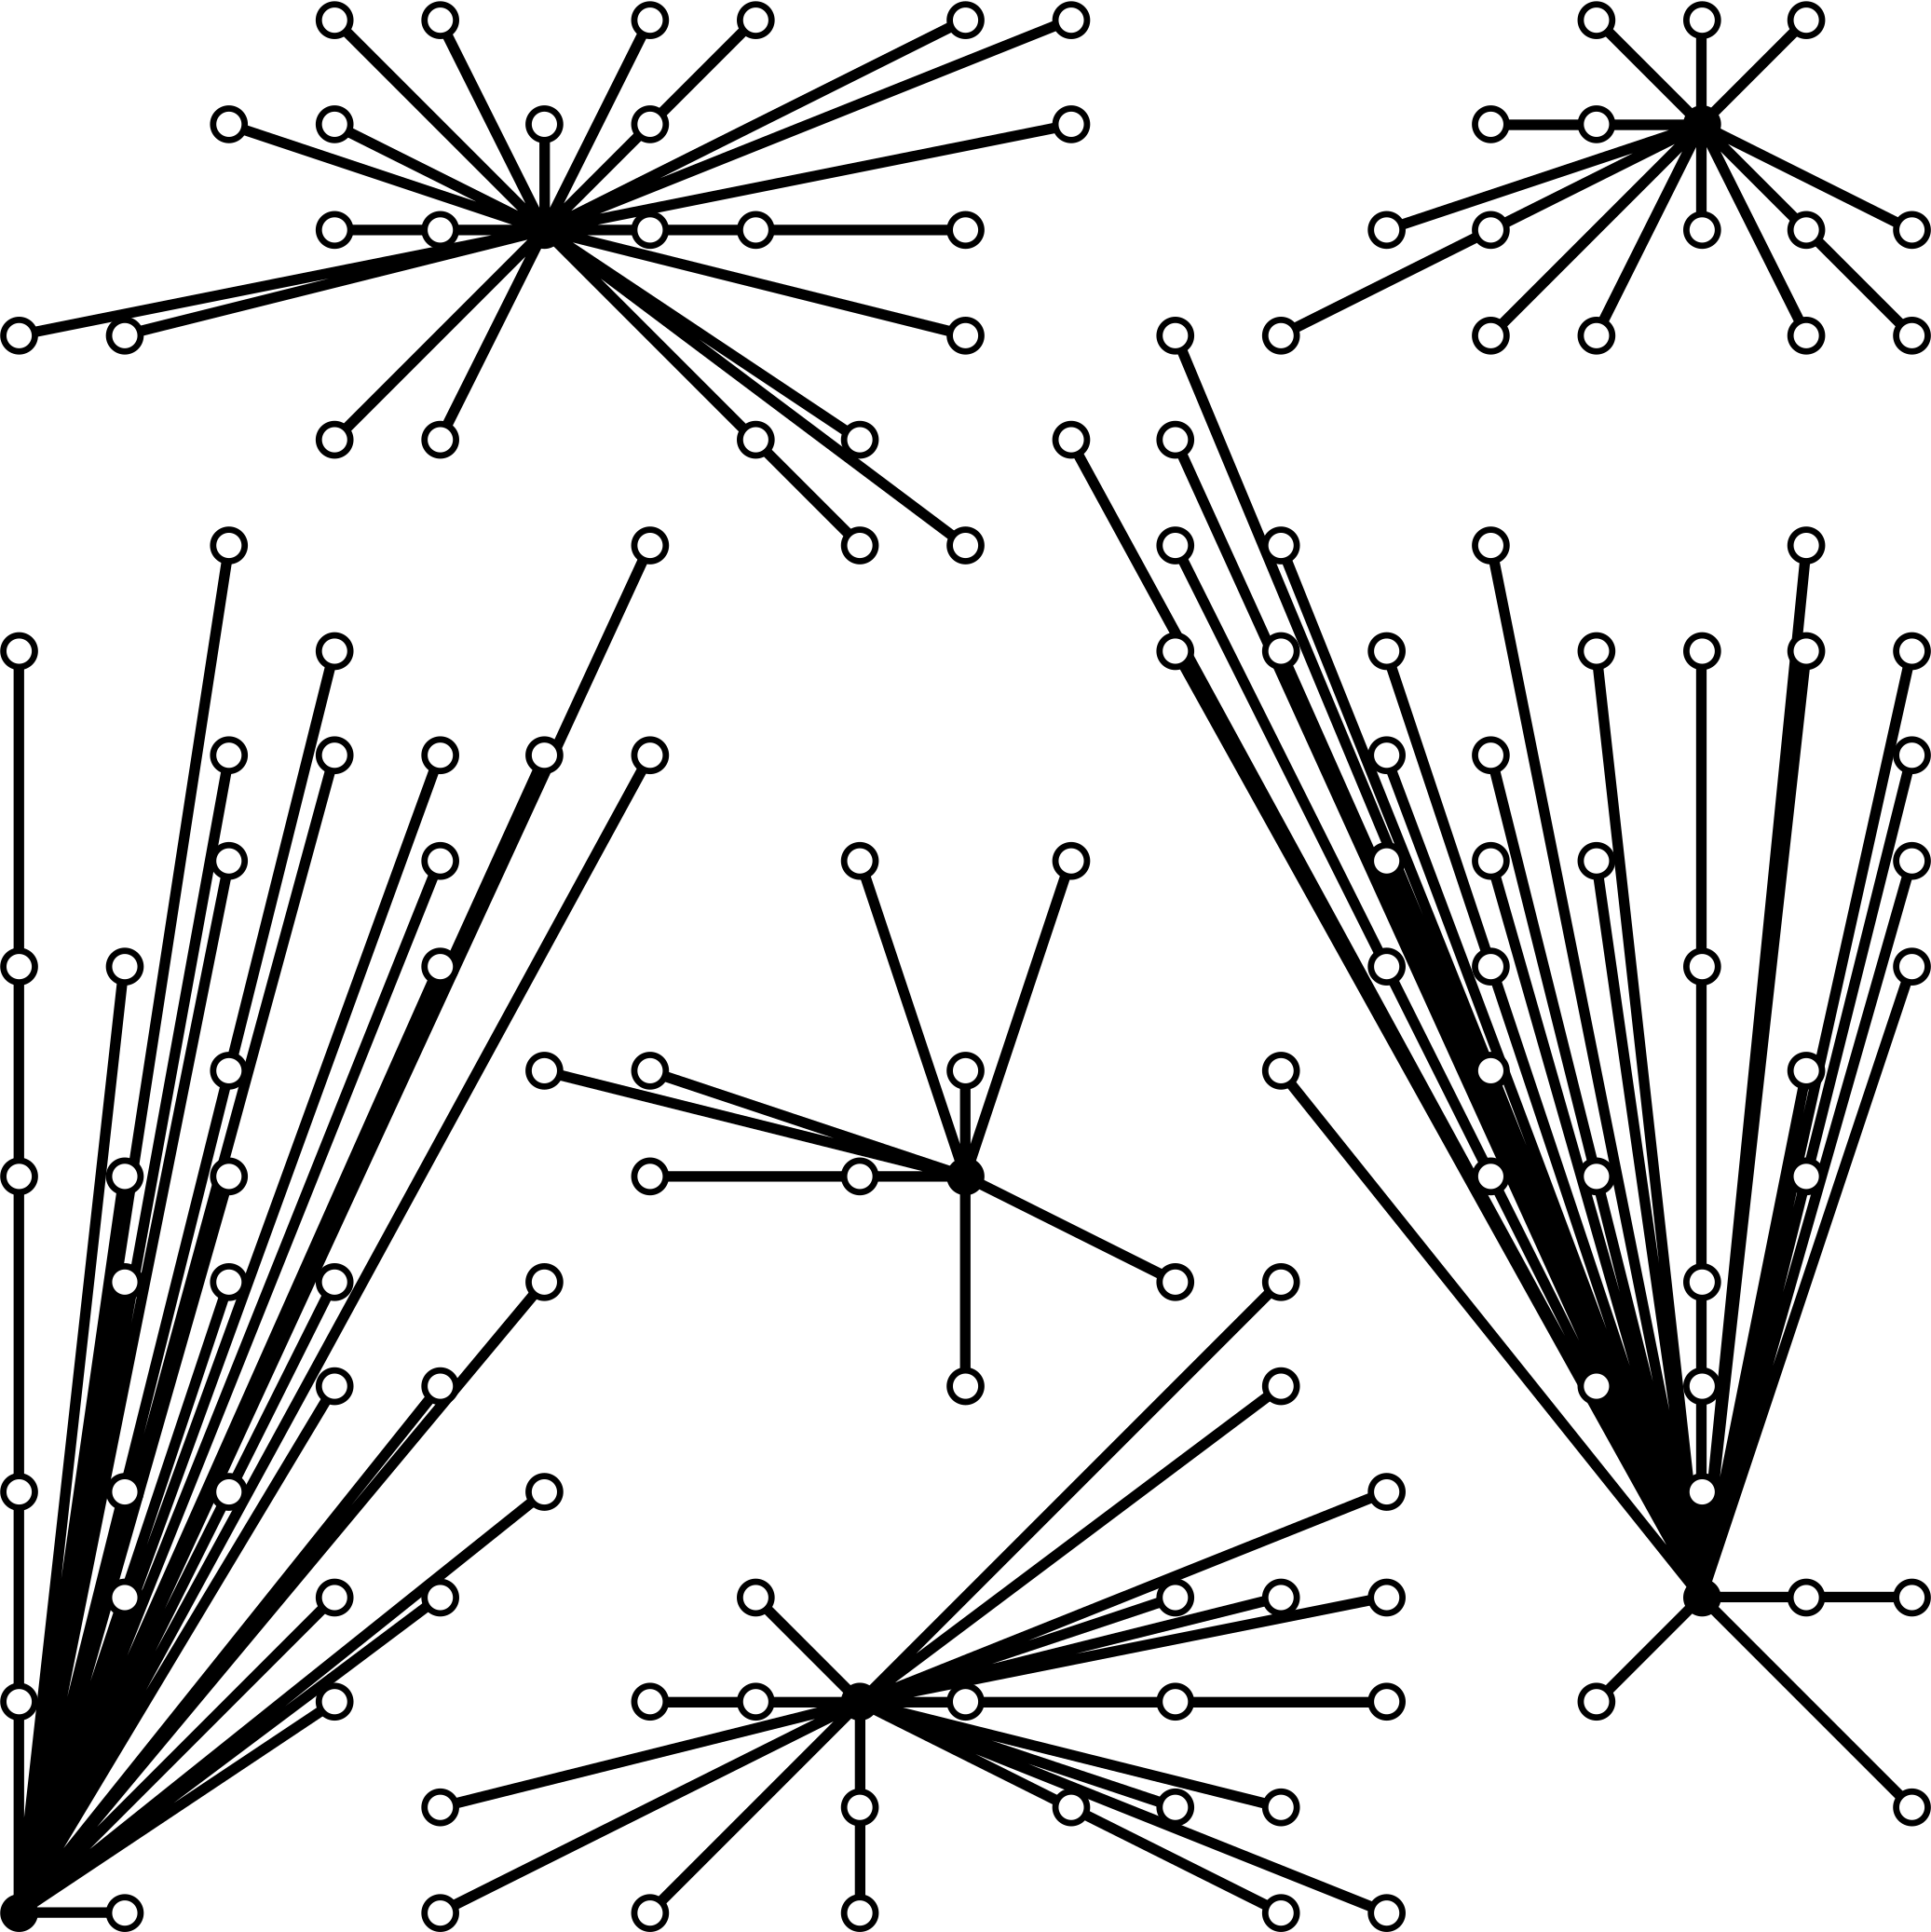
\includegraphics[width=\linewidth]{asset/mcl_iter_5.png}
    \subcaption{Converged transition matrix \(\lim_{\lambda \rightarrow \infty} \mathcal{M}^{(\lambda)}\). The cluster regions are apparent here.}
    \label{fig:mcl_iter_6}
  \end{subfigure}
  \hspace{0.5cm}

  \vspace{0.3cm}

  \caption{Source~\cite{mcl}. An intuitive demonstration of MCL applied on a sparse weighted graph. Each diagram is a depiction of the graph at different MCL iterations. The intensity of edge shades are proportional to the similarity or correlation of the linked vertex pair. Darker shades imply higher similarity, and conversely, lighter shades imply lower similarity.}
  \label{fig:mcl_iter}

\end{figure}

\subsection{Computational Overhead}

Like before, suppose that the transition matrix has shape \((n, n)\), while the
expansion parameter \(\epsilon\) is set to \(2\), a common design choice in MCL
literature. Each iteration consists of expansion (matrix squaring), pruning,
inflation, and normalization. For dense matrices, standard matrix
multiplication requires \(2 n^3 - n^2\) floating-point operations: each of the
\(n^2\) output entries requires \(n\) multiplications and \(n-1\) additions.
Inflation and normalization each contribute \(\mathcal{O}(n^2)\) operations;
specifically, inflation with non-integer exponent \(r>1\) costs
\(\sim 10 n^2\) FLOPs (assuming 10 FLOPs per elementwise exponentiation with
non-integer exponent), while normalization incurs \(n^2 - n\) FLOPs for column
sums and divisions. The termination criterion, evaluating the Frobenius norm
difference between successive matrices, adds roughly \(3n^2\) FLOPs per
iteration. Collectively, dense MCL requires \(\mathcal{O}(n^3)\) operations per
iteration, dominated by the expansion step, and consumes \(\mathcal{O}(n^2)\)
memory to store the full transition matrix. For example, given that each
element takes 32-bits, with \(10^5\) vertices in the graph, the memory reserved
for the transition matrix throughout the MCL runtime is \(\sim 37.25 \
\text{GiB}\). This renders dense MCL impractical for graphs with more than a frew thousand vertices, as the cubic growth quickly becomes prohivitive.
% Justification.
%\begin{align*}
%  (10^5)^2 \cdot 32 \ \text{bits} = 4 \cdot 10^{10} \ \text{bytes} = \dfrac{4 \cdot 10^{10}}{(2^{10})^3} \ \text{GiB} \approx 37.2529 \ \text{GiB}.
%\end{align*}

However, PSSNs are normally very sparse and this sparsity significantly reduces
the computational cost compared to \(\mathcal{O}(n^3)\) since operations
involving zero entries require no arithmetic operation and therefore take a
trivial number of cycles. This positive computational effect is reinforced by the pruning
operation at each subsequent MCL iteration. Therefore, we may accept that each column retains at most \(k_0: k_0 > 0\) non-zero
entries, where \(k_0\) can be influenced by the pruning threshold and is
typically much smaller than \(n\) in sparse PSSNs. Quantity \(k_0 \ll n\), often called
the \textit{average dimension}, determines the complexity of sparse operations.
For sparse matrices with average dimension \(k_0\), the computation of output column \(q\) is
\begin{align}
  \texttt{w}_{\cdot, q}^{(\lambda)}
  & = \mathcal{M}^{(\lambda-1)} \cdot \mathcal{M}^{(\lambda-1)}_{\cdot, q}
  \nonumber
  \\
  & = \sum_{k = 1}^{n} (\mathcal{M}^{(\lambda-1)}_{\cdot, k} \cdot \mathcal{M}^{(\lambda-1)}_{k, q})
  \nonumber
  \\
  & = \sum_{k = 1}^{k_0} (\mathcal{M}^{(\lambda-1)}_{\cdot, \xi_k} \cdot \mathcal{M}^{(\lambda-1)}_{\xi_k, q}).
  \label{eq:sparseExpansionCol}
\end{align}

The total number of elementary, non-zero computations becomes apparent in Eq~\ref{eq:sparseExpansionCol}. On that basis, the computation of each output column costs
\[
  \underbrace{k_0^2}_{\text{\# of multiplications}} + \ \ \ \ \underbrace{k_0 \cdot (k_0 - 1)}_{\text{\# of additions}} \ \ \text{FLOPs} = 2k_0^2 - k_0 \ \text{FLOPs}.
\]
This cost is repeated over all output columns \(n\). As a result, expansion
requires \(\mathcal{O}(n k_0^2)\) operations in total, while pruning,
inflation, and normalization each requires \(\mathcal{O}(n k_0)\) operations,
reducing the overall computational requirement down to \(\mathcal{O}(n
k_0^2)\). Memory consumption is also reduced down to \(\mathcal{O}(n k_0)\)
since the transition matrix may be stored in a compressed sparse format.
Fig.~\ref{fig:complexity} highlights the complexity advantage for
representative \(k_0\) values.

\begin{figure}[htbp]
  \centering
  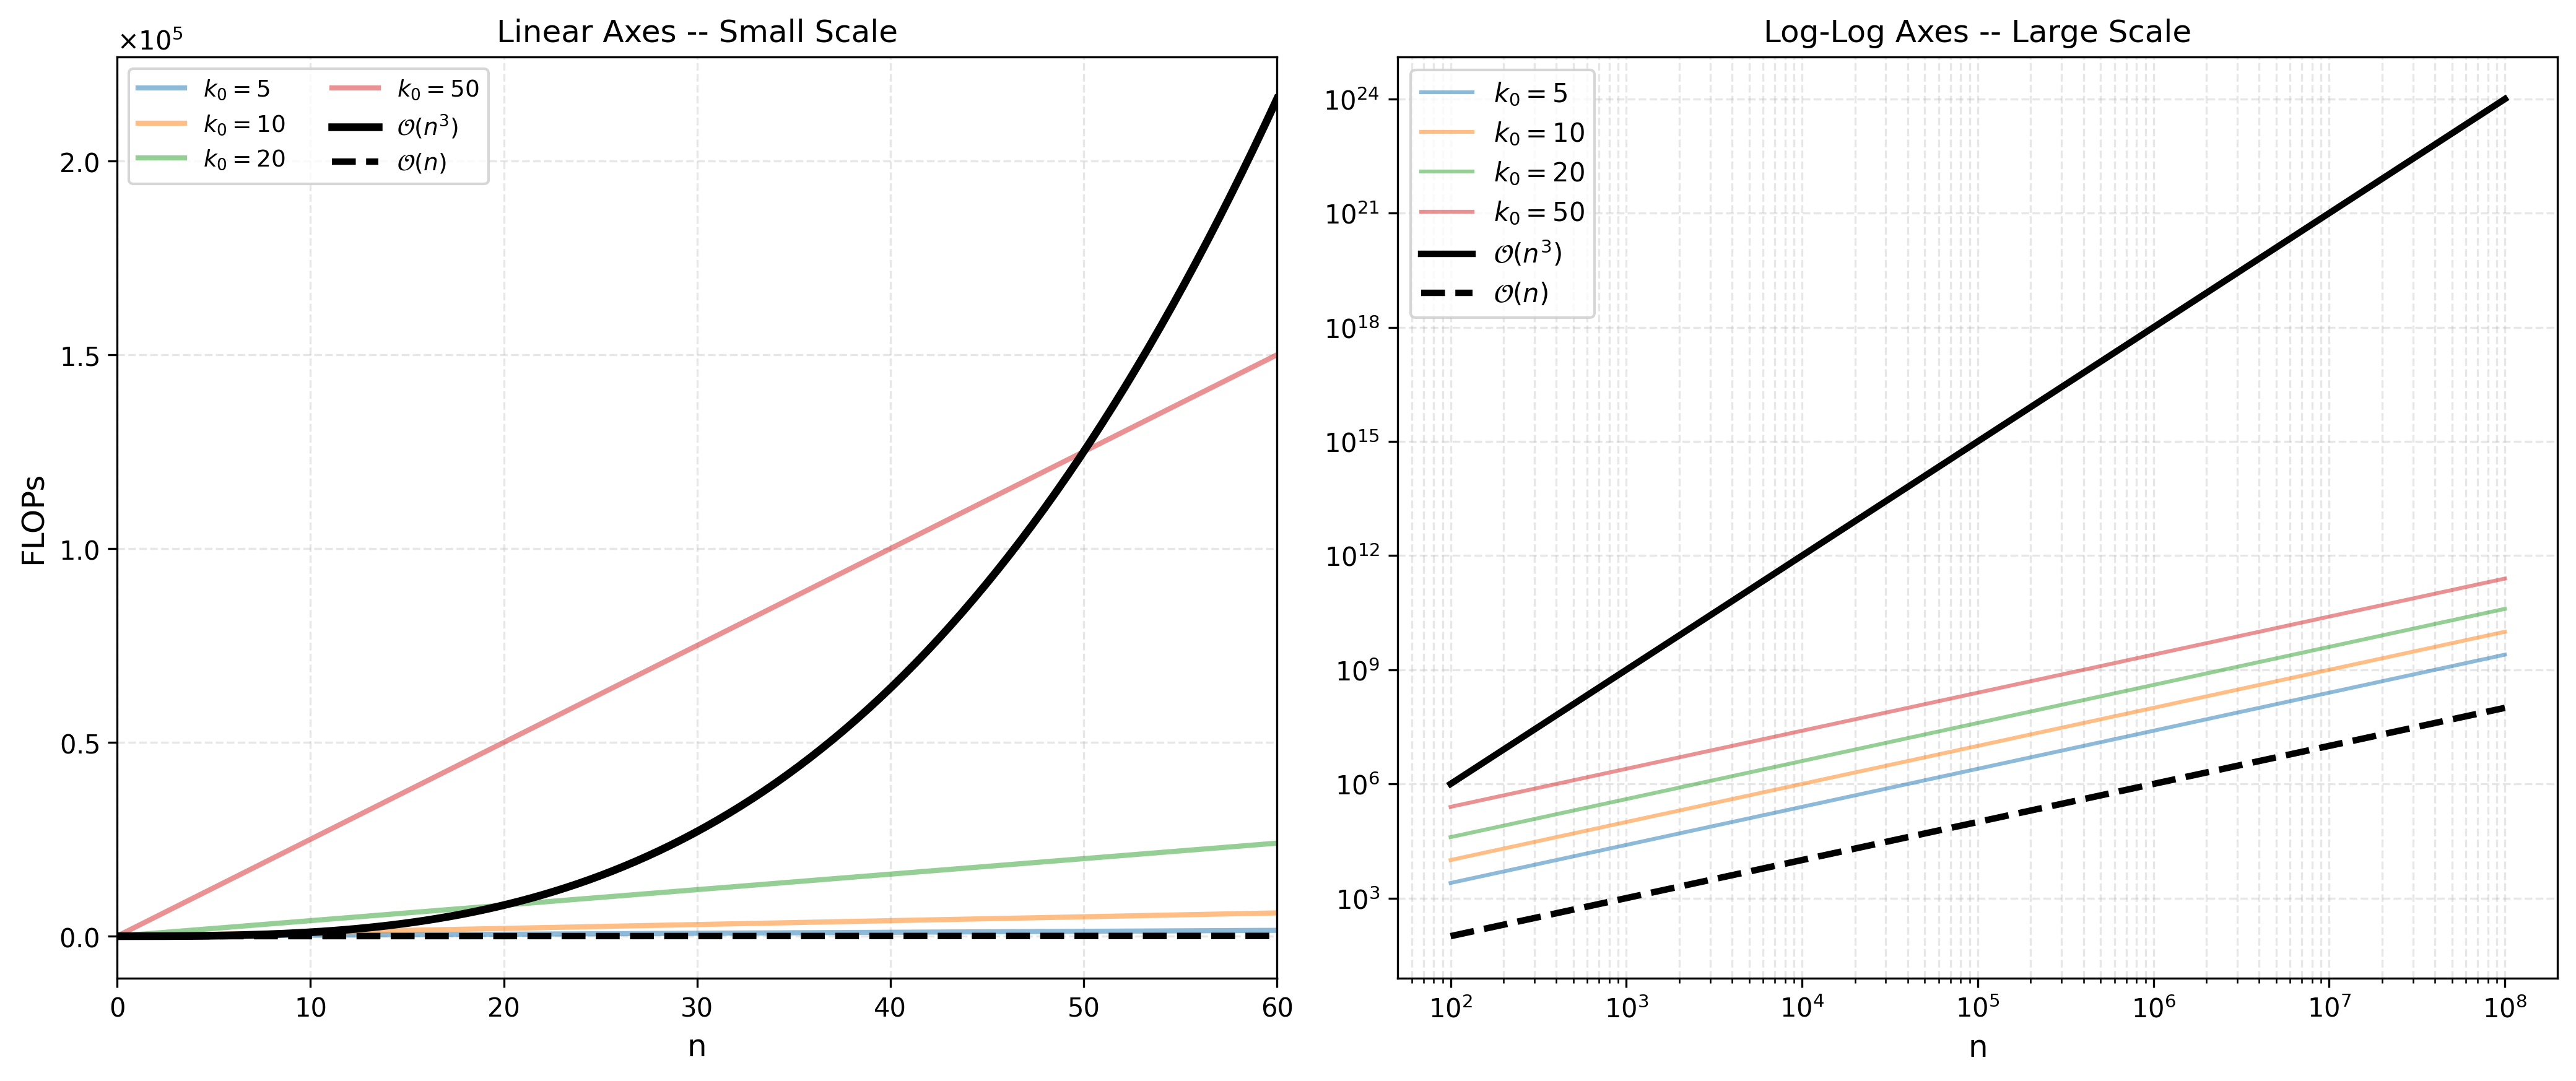
\includegraphics[width=1\linewidth]{asset/complexity.png}
  \caption{Complexity of sparse expansion \(\mathcal{O}(n k_0^2)\)
  compared against dense for \(k_0 \in \{5, 10, 20, 50 \}\) shown in color. The
  left plot uses linear axes to emphasize curvature at small \(n\), while the
  right plot uses log-log (base \(10\)) axes to illustrate scaling across many
  orders of magnitude.}
  \label{fig:complexity}
\end{figure}

Thus, in the numerical example where we assumed \(10^5\) vertices, if we
impose that only \(1 \%\) of the edges are non-zero, then the average
dimension \(k_0\) is \(10^3\). Therefore, the entire graph can be compressed
to an object reserving \(\sim 372.5 \ \text{MiB} \ll 37.25 \ \text{GiB}\)
which is a huge improvement when compared to the previous unoptimized
approach.

  \cleardoublepage
  \section{Method}
\chead{\thesection. Method}

The primary objective of this work is to compare two MCL-based clustering
methods on large-scale protein sequence datasets using Protein Sequence
Similarity Networks (PSSNs). The adopted workflow follows the CGG Toolkit
\cite{cggToolkit} framework and its flow diagram is illustrated in
Fig.~\ref{fig:workhigh}. Along with the clustering analysis, a qualitative study
is performed to characterize each dataset, including frequency diagrams of
residue distributions and sequence lengths, as well as heatmaps of adjacency
matrices.

Initially, protein sequences are curated using a standardized preprocessing
pipeline to ensure unique sequence identification. Low-complexity sequence
regions are then masked to prevent bias in subsequent sequence similarity
scoring. Masking low-complexity regions is a standard preprocessing step to
avoid spurious sequence similarity matches \cite{wootton1996seg}. After
applying a local sequence aligner, the computed sequence scores are used to
construct a PSSN. In the resulting graph, vertices correspond to protein
sequences and weighted edges encode pairwise similarity.

The primary contribution lies in the application and comparison of
reproducible, interpretable and scalable flow-based graph clustering methods,
specifically the Markov Cluster Algorithm (MCL) and its high performance
variant HipMCL, to cluster the produced PSSN into groups of homologous
proteins. The comparison evaluates each method's computational feasibility in
terms of peak memory usage and runtime in a single node, providing insight into
their scalability on large-scale protein sequence datasets.

% 600%
\begin{figure}[htbp]
  \centering
  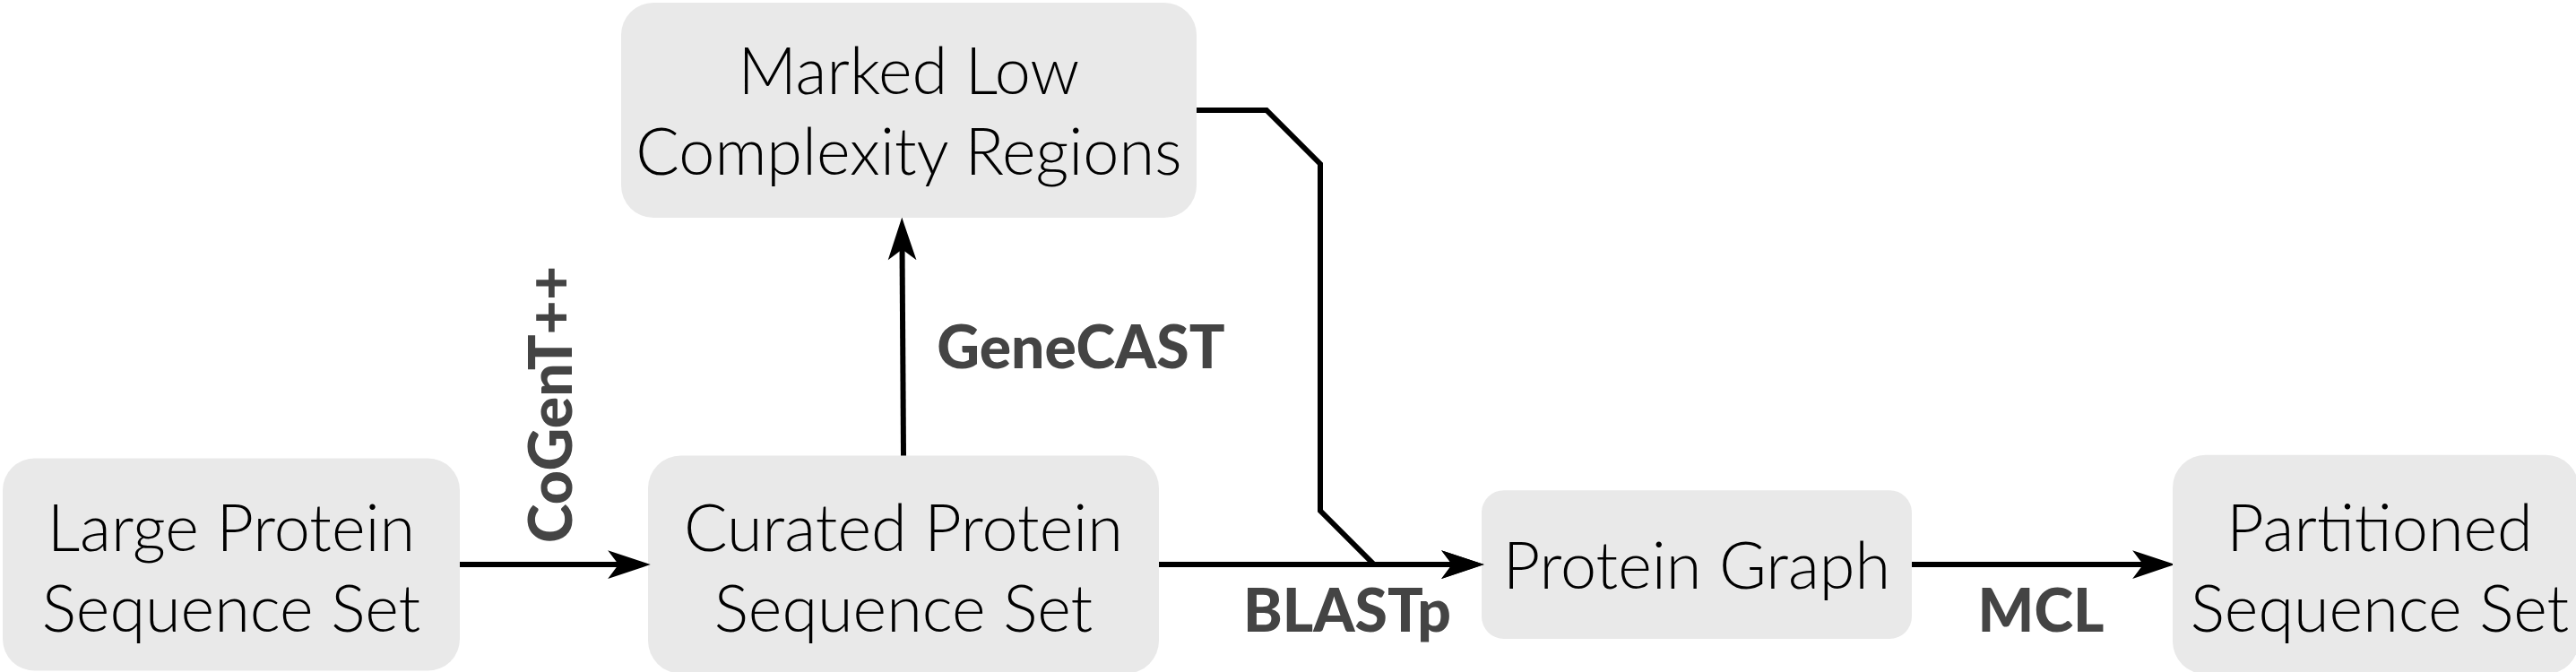
\includegraphics[width=1\linewidth]{asset/workhigh.png}
  \caption{Overview of the protein clustering workflow based on the CGG Toolkit. Each node represents a data object, and each directed edge denotes a transformation.}
  \label{fig:workhigh}
\end{figure}

\subsection{Data}

\subsubsection{Raw Data}

The data used in this project were protein sequences obtained from UniProt
\cite{uniprot}, a comprehensive repository maintained by the European
Bioinformatics Institute (EBI), the SIB Swiss Institute of Bioinformatics, and
the Protein Information Resource (PIR). For this thesis, the datasets were
drawn from UniProtKB, one of the three major database resources of UniProt.
Specifically, a large collection of FASTA records was obtained from UniProtKB
release 2025 April 02. Since the current work is limited to the analysis of
protein molecules, non-protein data (e.g., nucleic
acid sequences) were discarded. The final parsed dataset consists entirely of
curated \textit{reference proteomes}.

Reference proteomes are representative, non-redundant sets of protein sequences
selected to cover well-studied model organisms and species of biomedical or
phylogenetic interest. Each reference proteome includes canonical protein
sequences and, where available, additional isoforms or variant sequences, all
provided in standard FASTA format. Therefore, the raw data consists
exclusively of protein FASTA files obtained from the UniProt FTP
repository\footnote{\url{https://ftp.uniprot.org/pub/databases/uniprot/previous_major_releases/release-2025_02}}.
Viral reference proteomes were excluded to maintain taxonomic consistency, as
viruses differ fundamentally from cellular organisms in their evolutionary
patterns, and protein sequence characteristics. After discarding the viral proteomes, the distribution of obtained sequences per superkingdom is displayed in Table~\ref{tab:superkingdomDistribution}.

\begin{table}[htbp]
	\centering
	\caption{Distribution of proteomes and protein records in UniProtKB by taxonomic superkingdom.}
	\begin{tabular}{ccc}
		\toprule
		\textbf{Superkingdom} & \textbf{\# Proteomes} & \textbf{\# Protein Records} \\
		\midrule
		\arrayrulecolor{gray!50}
		Archaea & 303 & 750,976 \\
    \midrule
		Bacteria & 9,084 & 35,298,460 \\
		\midrule
		Eukaryota & 2,740 & 46,079,603 \\
		\arrayrulecolor{black}
		\midrule
		\textbf{Total} & 12,127 & 82,129,039 \\
    \bottomrule
	\end{tabular}
	\label{tab:superkingdomDistribution}
\end{table}

\subsubsection{FASTA Format}

Protein sequences were provided in standard FASTA format, a plain-text
representation for biological sequences. Each FASTA record consists of a single
header line followed by one or more lines encoding the sequence. 

Specifically, a FASTA record has the following format:

\begin{plaintext}
>HEADER[|DESCRIPTION]
SEQ_BLOCK
\end{plaintext}

\begin{table}[htbp]
	\centering
	\caption{Components of any FASTA record.}
	\begin{tabular}{p{3cm} p{10cm}}
		\toprule
		\textbf{Placeholder} & \textbf{Description} \\
    \midrule
		\texttt{HEADER} & A sequence identifier. Its syntax and semantics are database-specific (e.g., UniProt), and uniqueness is guaranteed only within the originating database. \\
		\arrayrulecolor{gray!50}
    \midrule
		\texttt{|DESCRIPTION} & Optional field. \texttt{|} is a literal character. Additional annotation fields, typically separated by spaces or pipe (\texttt{|}) characters, providing metadata such as protein name or organism. \\
		\midrule
		\texttt{SEQ\_BLOCK} & The biological sequence encoded using single-letter residue codes. Sequence lines may be wrapped and are interpreted as a contiguous sequence. \\
		\arrayrulecolor{black}
    \bottomrule
	\end{tabular}
	\label{tab:fastaComponents}
\end{table}

Observe Table~\ref{tab:fastaComponents} for the semantics of each component of
the aforementioned formatting. A FASTA file may contain more than one record.
FASTA files in this study contain protein sequences only. Common file
extensions include \texttt{.fasta}, \texttt{.fa}, and \texttt{.faa}.

\subsubsection{Curated Data}

The protein sequences obtained from UniProtKB were further processed based on
the CoGenT++ \cite{cogent0, cogent1} format to produce a curated dataset for
downstream tasks such as clustering. This process of curation involves the
systematic prefixing and standardization of the FASTA header. It ensures
uniqueness across all sequences using a compact identifier while encoding
additional globally identifiable metadata in a consistent format, while
preserving the initial header of the raw FASTA record.

Each FASTA record that is subjected to this curation follows the template:

\begin{plaintext}
>PROTEOMEID-TAXID-TRUNC_NAME-YEAR-PROT_CNT-SUPERKINGDOM-SEQ_CNT OLD_ID[|DESCRIPTION]
SEQ_BLOCK
\end{plaintext}

The following example is a FASTA record after being subjected to CoGenT++
curation, holding the protein called \textit{Chemokine-like Factor}. It
represents a sequence of amino acid residues originating from the human
proteome.

\begin{table}
  \centering
  \caption{Components of a CoGenT++ curated FASTA record.}
  \begin{tabular}{p{3cm} p{7cm} p{4.3cm}}
		\toprule
		\textbf{Placeholder} & \textbf{Description} & \textbf{Example} \\
    \midrule
		\texttt{PROTEOMEID} & UniProt reference proteome identifier. Each corresponds to exactly one \texttt{TAXID}. & \texttt{UP000005640} \\
		\arrayrulecolor{gray!50}
		\midrule
		\texttt{TAXID} & 8-digit zero-padded NCBI taxonomy ID of the source organism. & \texttt{00009606} \\
		\midrule
		\texttt{TRUNC\_NAME} & Truncated protein or gene name derived from the original header. & \texttt{Homo\_sapi} \\
		\midrule
		\texttt{YEAR} & Dataset release year or batch number. & \texttt{26} \\
		\midrule
		\texttt{PROT\_CNT} & 6-digit zero-padded per-superkingdom sequence counter starting from \texttt{000001}. & \texttt{000594} \\
		\midrule
		\texttt{SUPERKINGDOM} & Single-letter code for proteome's superkingdom (A = Archaea, B = Bacteria, E = Eukaryota). & \texttt{E} \\
		\midrule
		\texttt{SEQ\_CNT} & 6-digit zero-padded per-proteome sequence counter starting from \texttt{000001}. & \texttt{000996} \\
		\midrule
		\texttt{OLD\_ID} & Original UniProt FASTA identifier, preserved for traceability. & \texttt{sp|Q9UBR5|CKLF\_HUMAN} \\
		\midrule
		\texttt{|DESCRIPTION} & Optional metadata from the original header. & \texttt{Chemokine\dots SV=1} \\
		\midrule
		\texttt{SEQ\_BLOCK} & Amino-acid sequence, identical to the raw data. & See FASTA sequence. \\
		\arrayrulecolor{black}
    \bottomrule
  \end{tabular}
  \label{tab:curatedFastaComponents}
\end{table}

\begin{plaintext}
>UP000005640-00009606-Homo_sapi-26-000594-E-000996 sp|Q9UBR5|CKLF_HUMAN Chemokine-like factor OS=Homo sapiens OX=9606 GN=CKLF PE=1 SV=1
MDNVQPKIKHRPFCFSVKGHVKMLRLALTVTSMTFFIIAQAPEPYIVITGFEVTVILFFI
LLYVLRLDRLMKWLFWPLLDIINSLVTTVFMLIVSVLALIPETTTLTVGGGVFALVTAVC
CLADGALIYRKLLFNPSGPYQKKPVHEKKEVL
\end{plaintext}

Observe Table~\ref{tab:curatedFastaComponents} for the semantics of each
component of the aforementioned formatting. All sequences and headers remain
consistent with the FASTA format without disposing UniProt's annotations. These
principles are designed to facilitate reproducible, transferable and scalable
biological sequence analysis workflows such as the one outlined in the project
of the CGG Toolkit, making it suitable for the current protein analysis
workflow (observe Fig.~\ref{fig:workhigh}).

The resulting dataset will be referred to as \texttt{ref\_prot} throughout this study. Additionally, subsets of \texttt{ref\_prot} are isolated to investigate
\begin{itemize}
  \item The computational requirements of the clustering workflow, or
  \item A qualitative analysis of specific organisms.
\end{itemize}
In total, 13 additional subsets of \texttt{ref\_prot} were separately
analysed (observe Table~\ref{tab:dataStats}). It is worth noting that not all
pairs of these subsets are disjoint. Also, each dataset is assigned an
identifier. For each of these datasets, the identifier will be used as a
basename for all files tied to it, e.g., for the dataset
\texttt{ref\_prot}, its FASTA file is named as
\texttt{ref\_prot.fasta} and its partition \texttt{ref\_prot.cl}.

\begin{table}[htbp]
  \centering
  \caption{Subsets of \texttt{ref\_prot}. The column \textbf{Cmp} refers to whether that subset was utilized for the clustering analysis, while \textbf{Qlt} refers to qualitative analysis. Also, \textbf{Seq Len} and \textbf{Rec Cnt} refer to the protein length and record count corresponding to the length that appears most frequently. Finally, the \textbf{Size} column lists the number of records per dataset.}
  \begin{tabular}{ccc cc cc}
    \toprule
    \multicolumn{3}{c}{\textbf{General Data Information}} & \multicolumn{2}{c}{\textbf{Most Freq Length}} & \multicolumn{2}{c}{\textbf{Analysis}} \\
    \arrayrulecolor{gray!50}
    \midrule
    \arrayrulecolor{black}
    \textbf{Identifier} & \textbf{Size} & \textbf{Tax ID} & \textbf{Seq Len} & \textbf{Rec Cnt} & \textbf{Cmp} & \textbf{Qlt} \\
    \midrule
    \texttt{homo\_sapi} & 20,647 & 00009606 & 117 & 109 & \ding{51} & \ding{51} \\
    \arrayrulecolor{gray!50}
    \midrule
    \texttt{arab\_thal} & 27,448 & 00003702 & 256 & 75 & \textcolor{gray}{\ding{53}} & \ding{51} \\
    \midrule
    \texttt{carn\_malt} & 3,539 & 01234679 & 216 & 19 & \textcolor{gray}{\ding{53}} & \ding{51} \\
    \midrule
    \texttt{dani\_reri} & 26,728 & 00007955 & 257 & 70 & \textcolor{gray}{\ding{53}} & \ding{51} \\
    \midrule
    \texttt{sacc\_cere} & 6,065 & 00559292 & 440 & 40 & \textcolor{gray}{\ding{53}} & \ding{51} \\
    \midrule
    \texttt{hds\_prot} & 53,440 & \textcolor{gray}{N/A} & 312 & 155 & \ding{51} & \ding{51} \\
    \midrule
    \texttt{hac\_prot} & 51,634 & \textcolor{gray}{N/A} & 117 & 168 & \ding{51} & \ding{51} \\
    \midrule
    \texttt{hac\_prot\_small} & 18,002 & \textcolor{gray}{N/A} & \textcolor{gray}{N/A} & \textcolor{gray}{N/A} & \textcolor{gray}{\ding{53}} & \ding{51} \\
    \midrule
    \texttt{hds\_prot\_small} & 22,547 & \textcolor{gray}{N/A} & \textcolor{gray}{N/A} & \textcolor{gray}{N/A} & \textcolor{gray}{\ding{53}} & \ding{51} \\
    \midrule
    \texttt{archaea\_medium} & 378,303 & \textcolor{gray}{N/A} & \textcolor{gray}{N/A} & \textcolor{gray}{N/A} & \ding{51} & \textcolor{gray}{\ding{53}} \\
    \midrule
    \texttt{archaea} & 750,976 & \textcolor{gray}{N/A} & \textcolor{gray}{N/A} & \textcolor{gray}{N/A} & \ding{51} & \textcolor{gray}{\ding{53}} \\
    \midrule
    \texttt{bacteria\_tiny} & 2,972 K & \textcolor{gray}{N/A} & \textcolor{gray}{N/A} & \textcolor{gray}{N/A} & \ding{51} & \ding{51} \\
    \midrule
    \texttt{bacteria} & 35,298 K & \textcolor{gray}{N/A} & \textcolor{gray}{N/A} & \textcolor{gray}{N/A} & \ding{51} & \textcolor{gray}{\ding{53}} \\
    \midrule
    \texttt{ref\_prot} & 82,129 K & \textcolor{gray}{N/A} & \textcolor{gray}{N/A} & \textcolor{gray}{N/A} & \ding{51} & \textcolor{gray}{\ding{53}} \\
    \arrayrulecolor{black}
    \bottomrule
  \end{tabular}
  \label{tab:dataStats}
\end{table}

The first five datasets of Table~\ref{tab:dataStats} are individual reference
proteomes: \texttt{homo\_sapi}, \texttt{arab\_thal}, \texttt{carn\_malt},
\texttt{dani\_reri}, and \texttt{sacc\_cere}. These correspond to human, plant,
bacterium, zebrafish, and yeast (fungus), respectively. These are collectively
used as a foundation for the qualitative analysis, since \texttt{hac\_prot},
\texttt{hds\_prot} are a concatenation of \(\{\)\texttt{homo\_sapi},
\texttt{arab\_thal}, \texttt{carn\_malt}\(\}\) and \(\{\)\texttt{homo\_sapi},
\texttt{dani\_reri}, \texttt{sacc\_cere}\(\}\), respectively. In the same
order, the sequence sets \texttt{hac\_prot\_small} and
\texttt{hds\_prot\_small} are subsets of the former pair, in a way that makes
the organism distribution more uniform for the similarity heatmaps.

\subsection{Graph-based Representation of Protein Sequences}

Protein sequences are variable-length symbolic objects defined over an amino
acid alphabet comprised of 20 monomeric units (observe Table~\ref{tab:amino_acids}). Since the current task is
to partition the sequence set \(\mathscr{V}\), we first construct a numerical
representation of the dataset. 

In this work, similarities are measured using BLASTp \cite{blast}, a widely used sequence aligner, through the
DIAMOND tool \cite{diamond}. We have utilized DIAMOND's git repository\footnote{\url{https://github.com/bbuchfink/diamond} from the codebase with commit hash \texttt{0x25165b5}.}. BLASTp performs local sequence alignment on protein sequences. In this case, BLASTp
utilizes the 20 x 20 substitution matrix called BLOSUM62 (observe the
\texttt{-{}-matrix} parameter) to perform the alignment. A substitution matrix is a symmetric matrix that defines
scores for aligning amino acid residue pairs based on observed evolutionary
substitution patterns, assigning positive scores to substitutions between
similar residues (e.g., Isoleucine and Leucine) and negative scores to unlikely
substitutions. BLASTp takes a pair of sequences as input and, after
sequence alignment, it produces a set of scores that express pairwise
similarity. Bulk processing is performed in an all-versus-all manner over
\(\mathscr{V}\), from which only the top 25 optimal alignment pairs are kept
(through \texttt{-{}-max-target-seqs}).
To model pairwise similarity, we use the maximum bit score that reflects the
strength of the match, independent of the input database. Another important output
value of BLASTp that is utilized is the input pair's E-value, a statistical
measure of the expected number of matches of similar quality that would occur
by chance when comparing against a database of reference proteins. A lower
E-value corresponds to a more statistically significant similarity, indicating
a stronger relationship of the corresponding sequence pair.

A known issue in local sequence alignment is the presence of low-entropy or
repeating patterns, which can lead to artificially inflated similarity scores.
For example, the subsequences \texttt{GGGGGG} and \texttt{PEPEPEPEPE} are
frequently encountered in existing protein sequences. Since sequence alignment is
performed locally, these may match many unrelated sequences solely due to
compositional bias, producing high maximum bit scores and low E-values despite
lacking evolutionary relatedness. Such motifs are called
\textit{low-complexity} and to mitigate the negative effect of their
repetition, sequences are preprocessed based on GeneCAST \cite{genecast}, an
algorithm that identifies and masks low-complexity regions prior to alignment.
The utilized implementation of GeneCAST relied on \texttt{genecast\_1}, a
specific tool originating from the official CGG Toolkit's
repository\footnote{\url{https://github.com/bcpl-certh/cgg-toolkit/tree/main/1_genecast}
at commit \texttt{0x92243d0}.}. The only parameter that is overridden is
\texttt{MAXSEQLEN} from the file \texttt{:/genecast\_1/cast.c}, which is set to
\texttt{50000}, since the input data contain sequences of length greater than
the default value. This parameter controls the maximum sequence length that can
be processed from the input sample. The rest of the configuration was preserved
to its default settings. Also, the masking is performed by simply replacing the
identified low-complexity local region with an equal length of multiple
\(\texttt{X}\) characters. The character \(\texttt{X}\) is a special token that
does not belong in the protein residue alphabet and is therefore unrecognizable
by BLASTp. For example, the motif \texttt{ASSSGAGAAAAAAAA} that appears in

\begin{plaintext}
>UP000005640-00009606-Homo_sapi-26-000594-E-000041 sp|Q08AG7... PE=1 SV=2
M$\texttt{\underline{ASSSGAGAAAAAAAA}}$NLNAVRETMDVLLEISRILNTGLDMETLSICVRLCEQGINPEAL
SSVIKELRKATEALKAAENMTS
\end{plaintext}

is subsequently localized by GeneCAST and classified as a low-complexity region relative to that specific sequence. Then, the sequence is modified into

\begin{plaintext}
>UP000005640-00009606-Homo_sapi-26-000594-E-000041 sp|Q08AG7... PE=1 SV=2 
M$\texttt{\underline{XSSSGXGXXXXXXXX}}$NLNAVRETMDVLLEISRILNTGLDMETLSICVRLCEQGINPEAL 
SSVIKELRKATEALKAAENMTS
\end{plaintext}

Subsequently, these low complexity regions do not contribute to the scoring of
a pair's alignment, as they always mismatch with the original residue tokens.
The masking is applied to the input FASTA file using the following command:
\begin{plaintext}[numbers=none]
cast sample.fasta > sample.casta
\end{plaintext}
after masking, an all‑vs‑all sequence alignment is performed with diamond:
\begin{plaintext}
diamond blastp --query sample.casta --db sample.fasta --out sample.pairs --outfmt 6 qseqid sseqid bitscore evalue
\end{plaintext}
from the raw alignments, only statistically significant pairs (e‑value \(\leq\) 0.005) are retained, extracting the query id, subject id, and bit score:
\begin{plaintext}[numbers=none]
awk '$\textdollar$(NF) <= 0.005 {print $\textdollar$1, $\textdollar$2, $\textdollar$(NF-1)}' sample.pairs > sample.adj
\end{plaintext}
After the dataset is processed by GeneCAST and BLASTp, the resulting pairwise
similarity matrix is further sparsified by filtering out statistically
insignificant weights. In this case, the filtering is performed by setting the
E-value cutoff to \(5 \cdot 10^{-3}\), effectively keeping only the edges that
correspond to E-values smaller than or equal to the selected cutoff value. This
produces a sparse similarity representation of protein pairs comprising only
statistically significant relationships. The resulting file \texttt{sample.adj}
is a compact representation of the adjacency matrix \(\mathcal{A}\) containing
only the identifiers of the preserved protein pairs along with their similarity
values. Thus, each line has the following simple structure \texttt{S1\_ID
S2\_ID BITSCORE\_1\_2}. To demonstrate with an example, what follows below is
a segment of three lines from the \texttt{homo\_sapi.adj} file
\begin{plaintext}
UP000005640-00009606-Homo_sapi-26-000594-E-000003 UP000005640-00009606-Homo_sapi-26-000594-E-002855 69.3
UP000005640-00009606-Homo_sapi-26-000594-E-000003 UP000005640-00009606-Homo_sapi-26-000594-E-001453 62.4
UP000005640-00009606-Homo_sapi-26-000594-E-000003 UP000005640-00009606-Homo_sapi-26-000594-E-003006 61.2
\end{plaintext}

\subsection{Clustering}

Up to this point, we have demonstrated how the sparse weighted adjacency matrix
\(\mathcal{A}\) was constructed and encoded in the file \texttt{sample.adj}.
Together with the sequence dataset \(\mathscr{V}\) encoded in
\texttt{sample.fasta}, this pair of files defines a sparse
PSSN, serving as the input to the protein clustering stage.

Clustering is performed using the Markov Cluster Algorithm (MCL). Two
implementations were evaluated: the reference MCL \cite{mcl} via the
\texttt{mcl}\footnote{\url{https://github.com/micans/mcl} at commit
\texttt{0x8c99282}.} CLI tool and its high-performance variant HipMCL \cite{hipmcl}
via the \texttt{hipmcl}\footnote{\url{https://bitbucket.org/azadcse/hipmcl} at
commit \texttt{0xca6a4fb}.} tool. Both methods operate directly on the
constructed PSSN and partition the vertex set into a collection of disjoint
graph clusters (communities). The resulting partition is exported to a file
named \texttt{sample.cl}.

\subsubsection{MCL}

For clustering with the reference MCL implementation, the graph is first converted to MCL's native matrix format using \texttt{mcxload}:

\begin{plaintext}[numbers=none]
mcxload --stream-mirror -abc sample.adj -o sample.mci -write-tab sample.tab
\end{plaintext}

Here, \texttt{-abc} specifies the aforementioned pair-edge format of
\texttt{sample.adj}. The flag \texttt{-{}-stream-mirror} enforces symmetric
loading of the edge list, and \texttt{-write-tab} stores the mapping between
sequence identifiers and internal matrix indices for later reference.

Clustering is then performed on the converted graph using \texttt{mcl}:

\begin{plaintext}[numbers=none]
mcl sample.mci -I INFLATION -te 48 -use-tab sample.tab -o sample.cl
\end{plaintext}

The \texttt{-te 48} flag requests 48 worker threads, half of the total number
of virtual threads available on the compute node (96). The \texttt{-I} parameter sets the inflation value, which indirectly controls the
granularity of the resulting partition. The output is written to
\texttt{sample.cl}, where each line contains a whitespace-separated list of
protein identifiers belonging to a single cluster.

\subsubsection{HipMCL}

Clustering was also performed with \texttt{HipMCL}. Since the present study is
restricted to a single compute node, \texttt{HipMCL} is not used in a
distributed multi-node configuration for which it was designed. Instead, it
is executed locally on the PSSN through the command

\begin{plaintext}[numbers=none]
hipmcl -M sample.adj -I INFLATION -per-process-mem 16 -o sample.cl
\end{plaintext}

where \texttt{-M} specifies the weighted graph input, \texttt{-I INFLATION} is
the inflation parameter, and \texttt{-per-process-mem 16} reserves 16~GiB of
memory per process. The output of \texttt{HipMCL} is a partition of the input
vertex set into disjoint clusters, analogous to the output of standard MCL.

\subsubsection{Output processing and recorded measurements}

The raw clustering output of each method consists of one line per cluster, with
sequence identifiers separated by whitespace. Clusters are listed in decreasing
order with respect to cluster size. For example, for a sequence set
\(\mathscr{V}\) with identifiers \(\{\)\texttt{S01\_ID}, \dots,
\texttt{S16\_ID}\(\}\), a valid \texttt{sample.cl} file might contain:

\begin{plaintext}
S01_ID S02_ID S03_ID S04_ID
S05_ID S06_ID S07_ID S08_ID
S09_ID S10_ID S11_ID
S12_ID S13_ID
S14_ID S15_ID
S16_ID
\end{plaintext}

This shows that the sequences corresponding to the identifier collection
\(\{\)\texttt{S01\_ID, ..., S04\_ID}\(\}\) is a single cluster, \(\{\)\texttt{S05\_ID, ..., S08\_ID}\(\}\) is another cluster, and so on.

\subsection[Workflow \& \ Streamlined Implementation]{Workflow \& Streamlined Implementation}

The low-complexity masking, alignment, filtering, PSSN construction, and its
partitioning steps described above were integrated into a single executable
workflow called
\texttt{bioscflow}\footnote{\url{https://github.com/fl0wxr/bioscflow} at commit \texttt{0xc81d4e6}.}. The
tool is implemented in Python and orchestrates the execution of external
dependencies (GeneCAST, DIAMOND, MCL, HipMCL) while managing file paths,
intermediate data, and result logging. The workflow is designed for single-node
execution.

\texttt{bioscflow} is invoked from the command line with the following required parameters:

\begin{plaintext}[numbers=none]
python3 run.py --db data/raw/sample.fasta -I INFLATION --algorithm mcl
\end{plaintext}

The full interface is summarized below:

\begin{plaintext}
usage: run.py [-h] --db DB -I I --algorithm {mcl,hipmcl} [--nopreproc] [--debug]

bioscflow: Perform community detection on a sequence similarity network. The vertex weight is set as the bit score estimated from an all-vs-all local sequence alignment (BLASTp), applied on some set of user provided database of FASTA sequences.

options:
  -h, --help            show this help message and exit
  --db DB               Filepath of FASTA database (canonical directory path in
                        :/data/raw).
                        Warning: Each record header must start with a unique
                        identifier.
  -I I                  Inflation parameter of MCL.
  --algorithm {mcl,hipmcl}
                        Clustering algorithm to use.
                        |-> mcl: Reference MCL implementation
                        |-> hipmcl: HipMCL (single-node mode)
  --nopreproc           Disable preprocessing; apply community detection on an
                        already prepared adjacency matrix.
\end{plaintext}

For each run, \texttt{bioscflow} produces two outputs:

\begin{enumerate}
  \item A cluster file (\texttt{.cl}) where each line contains a whitespace-separated list of protein identifiers belonging to one cluster. Clusters are listed in decreasing order of size.
  \item A JSON session report containing metadata, runtime measurements, and exit codes for each pipeline stage with codenames \texttt{CAST}, \texttt{BLAST}, \texttt{FILTER} and \texttt{COMDET}, corresponding to GeneCAST, BLASTp, statistically significant edge filtering and community detection.
\end{enumerate}

An example session report is shown below:

\begin{plaintext}
{
  "algorithm": "mcl",
  "inflation": 2.5,
  "dataset_name": "sample",
  "dataset_size": 10000,
  "n_significant_edges": 45231,
  "n_clusters": 1250,
  "datetime": "d20250418t153022",
  "delta_t": 124.7,
  "delta_t_h": "02m:04s",
  "subprocess_id": ["CAST", "BLAST", "FILTER", "COMDET"],
  "exit_code_per_subprocess": [0, 0, 0, 0]
}
\end{plaintext}

For a visual overview of this entire workflow, observe Fig.~\ref{fig:work}.
Starting from the UniProtKB input, the figure shows all the involved steps,
namely the elimination of low-complexity regions, sequence alignment, PSSN
construction, clustering, a final output generation along with a potential use
case (downstream task). The workflow was applied to all datasets described in
the previous section. The following chapter reports the computational
performance and clustering outcomes obtained under varying inflation arguments
(\texttt{INFLATION}) and clustering algorithm choices between MCL and HipMCL.

% 600%
\begin{figure}[htbp]
  \centering
  \hspace*{-1.51cm}
\includegraphics[width=1.17\linewidth]{asset/work.png}
  \caption{Detailed view of the protein clustering workflow. FASTA header
  format is curated based on CoGenT++ while low-complexity regions are
  eliminated through GeneCAST. Next the FASTA sequence is subjected to sequence
  alignment based on BLASTp. Statistically significant alignments are
  preserved to construct a sparse PSSN, which is subsequently partitioned using
  MCL or HipMCL to identify protein communities. The protein language model
  (PLM) shown in the figure is included for conceptual context only and is not
  part of the implemented workflow.}
  \label{fig:work}
\end{figure}

\subsection{Qualitative Analysis}

As it was already shown in Table~\ref{tab:dataStats}, multiple subsets of
\texttt{ref\_prot} were selected for a qualitative analysis. Below we provide
the documentation of this analysis, while giving a brief description of the
motivation behind each component. The purpose of the qualitative analysis is to
characterize each of the five involved proteomes, and utilize them
as an intuitive use-case baseline to evaluate all the components that
constitute the clustering workflow. The basis of this analysis is a diverse set
of diagrams that capture semantic descriptors of the protein datasets and the
PSSN's features. These visual cues also serve as indicators for the integrity
of the components that constitute the clustering workflow (observe
Fig.~\ref{fig:work}). Specifically, we utilize heatmap images to display the
pairwise relationship accentuated by PSSNs, between proteomes of individual
organisms. Additionally, we display frequency diagrams of residue distributions
and sequence lengths that capture the distributional signature of the datasets
used to perform the scalability analysis. Finally, graph projections of
clustered proteins are shown, partitioned with respect to both TaxID ---
serving as a ground truth --- and by the communities produced by MCL.

To support the qualitative analysis, we constructed two composite
datasets: \texttt{hds\_prot\_small} and \texttt{hac\_prot\_small}. These are
subsets of the larger \texttt{hds\_prot} and \texttt{hac\_prot} datasets,
designed to be more uniformly distributed across their constituent proteomes.
This uniformity improves the interpretability of heatmaps and graph projections
by preventing any single proteome from dominating the layout. These datasets
are used exclusively for the adjacency matrix heatmaps and the similarity graph
projections. Separate plots --- sequence length distributions and amino acid bar
plots --- were generated from the original \texttt{hds\_prot} and
\texttt{hac\_prot} datasets and from the five individual proteomes
(\texttt{homo\_sapi}, \texttt{arab\_thal}, \texttt{carn\_malt},
\texttt{dani\_reri}, \texttt{sacc\_cere}) to provide complementary distributional
signatures.

Additionally, we analyze cluster size distributions by counting the number of
sequences per cluster from the output \texttt{.cl} files of MCL and HipMCL
runs. The dataset selected for this visualization is \texttt{bacteria\_tiny}.
These distributions are visualized as bar plots with bins.

To qualitatively validate the clusters produced by MCL, we retrieve
estimated three-dimensional structures from AlphaFold's Protein Structure Database\footnote{\url{https://alphafold.ebi.ac.uk}} for selected proteins.
From the clustering results on the \texttt{ref\_prot} dataset (inflation 2.5),
we select three clusters --- denoted r1, r4, and r22 --- representing maximum,
mild, and low taxonomic purity, respectively. For each selected cluster,
three proteins are selected by randomly shuffling the cluster and iteratively
testing candidates until the following constraints are satisfied: each
protein's length is near the cluster mean, and the three selected lengths
differ from one another. Structures are rendered as ribbon diagrams and
colored according to the predicted Local Distance Difference Test (pLDDT)
confidence metric \cite{plddt}. pLDDT is a per‑residue score ranging from 0 to
100, where higher values indicate greater local structural accuracy. Residues
with pLDDT > 90 are expected to be highly accurate, while values below 50
suggest disorder or very low confidence.

To assess the taxonomic composition of the resulting clusters, cluster purity
is computed. Let \(\mathscr{C} = \{C_1, \dots, C_k\}\) be the collection of
clusters produced by MCL, and let \(\text{tax}(p)\) be the TaxID of protein
\(p\). The purity of a single cluster \(C_j\) is defined as:

\begin{align*}
  \text{Purity}(C_j) = \frac{1}{|C_j|} \max \Big( \Big\{ \big| \{ p \in C_j : \text{tax}(p) = t \} \big| : \text{for every tax ID } t \Big\} \Big).
\end{align*}

Based on this measure, all clusters are ranked by their size (number of
proteins) and selected the top‑25 largest clusters. For each selected cluster,
we compute its purity as defined above, as well as its size (cardinality).
These values are visualized as a bar plot in
Fig.~\ref{fig:partition_composition}~(j), where cluster size is shown as blue
bars (left vertical axis), and purity as coral bars (right vertical axis).
Inside each blue bar of the same figure, the dominant TaxID and the number of
distinct TaxIDs in the cluster are indicated; inside each coral bar, the purity
percentage and the number of distinct TaxIDs are shown.

  \cleardoublepage
  \section{Results}
\chead{\thesection. Results}

\subsection{Scalability Analysis}

\subsubsection*{Runtime Environment}

Although HipMCL supports distributed execution, this study evaluates
single-node performance. The dataset fits within a single node's memory, and
single-node execution simplifies reproducibility while remaining sufficient for
the scale of the experiments.

The experiments reported in this thesis were executed on a single-node,
high-throughput, high-memory virtual server. The system runs Ubuntu 20.04.6
LTS and provides 96 logical CPUs, with approximately 971 GiB of RAM. The
reported processor model is an Intel Xeon Processor (Cascadelake)\footnote{CPU
information was obtained from the file content of \texttt{/proc/cpuinfo}.}.

\subsubsection*{Stress Test}

To evaluate the practical limits of MCL and HipMCL on a single node, we execute
both algorithms on datasets spanning three orders of magnitude in size, from
20K to 82M protein sequences. Table~\ref{tab:experimentsPalladium} reports
runtime, peak memory, and number of clusters for each configuration under two
inflation parameters (1.8 and 2.5).

For datasets up to 750K sequences, both algorithms complete within minutes.
HipMCL consistently consumes more memory than MCL (typically 2-4\(\times\)
higher) while producing slightly more clusters. Higher inflation (2.5)
generally reduces runtime and increases cluster count, consistent with its role
in accelerating convergence to a block-diagonal matrix.

We impose a runtime limit of 4 days per experiment. At the \texttt{bacteria}
dataset (35M sequences), HipMCL exceeds this limit and does not complete, while
MCL continues to produce results with multi-hour runtimes. For the largest
dataset, \texttt{ref\_prot} (82M sequences), MCL completes in 2–3 days using
approximately 440 GiB of memory at peak. Note that for MCL, generating the
\texttt{.mci} input file consumes approximately as much time as the prediction
phase itself. Experiments based on HipMCL surpass the 4-day limit on datasets
larger than 3M sequences. Therefore, the latter are labelled as failed and were
not documented.

\begin{table}[htbp]
  \footnotesize
  \hspace*{-5cm}
  \addtolength{\tabcolsep}{0pt}  % Column distance.
  \centering
\caption{Community detection experiments. The column \# \textbf{Edges} refers to the number of all statistically significant similarity measurements produced from the protein sequence aligner. \texttt{N/A} indicates that the experiment exceeded the runtime limit and was terminated without producing a result. Here, K denotes \(10^3\) while M denotes \(10^6\).}
  \begin{tabular}{ccccccrr}
    \toprule
    \textbf{Dataset} & \textbf{Size} & \textbf{\# Edges} & \textbf{Model} & \textbf{Inflation} & \textbf{\# Clusters} & \textbf{Time} & \textbf{Peak Mem.}\\
    \midrule
    \multirow{4}{*}{\texttt{homo\_sapi}} & \multirow{4}{*}{20.6 K} & \multirow{4}{*}{153,699}
        & MCL    & 1.8 & 8,969 & 1s:511ms & 49.05 MiB \\
    & & & HipMCL & 1.8 & 9,176 & 1s:446ms & 221.06 MiB \\
    & & & MCL    & 2.5 & 9,203 & 1s:207ms & 56.17 MiB \\
    & & & HipMCL & 2.5 & 9,435 & 1s:905ms & 184.20 MiB \\
    \arrayrulecolor{gray!50}  % Horizontal separator color.
    \midrule
    \multirow{4}{*}{\texttt{hac\_prot}} & \multirow{4}{*}{51.6 K} & \multirow{4}{*}{15,924}
        & MCL    & 1.8 & 10,309 & 1s:280ms & 52.87 MiB \\
    & & & HipMCL & 1.8 & 10,383 & 1s:305ms & 80.97 MiB \\
    & & & MCL    & 2.5 & 10,449 & 1s:077ms & 46.16 MiB \\
    & & & HipMCL & 2.5 & 10,539 & 0s:892ms & 61.26 MiB \\
    \midrule
    \multirow{4}{*}{\texttt{hds\_prot}} & \multirow{4}{*}{53.4 K} & \multirow{4}{*}{554,664}
        & MCL    & 1.8 & 10,379 & 1s:561ms & 72.02 MiB \\
    & & & HipMCL & 1.8 & 10,578 & 2s:206ms & 125.64 MiB \\
    & & & MCL    & 2.5 & 10,559 & 1s:316ms & 57.99 MiB \\
    & & & HipMCL & 2.5 & 10,793 & 1s:607ms & 116.96 MiB \\
    \midrule
    \multirow{4}{*}{\texttt{archaea\_medium}} & \multirow{4}{*}{378.3 K} & \multirow{4}{*}{6,498 K}
        & MCL    & 1.8 & 64,000 & 48s:020ms & 1.40 GiB \\
    & & & HipMCL & 1.8 & 68,091 & 58s:875ms & 6.98 GiB \\
    & & & MCL    & 2.5 & 68,328 & 38s:097ms & 1.35 GiB \\
    & & & HipMCL & 2.5 & 73,698 & 50s:230ms & 6.95 GiB \\
    \midrule
    \multirow{4}{*}{\texttt{archaea}} & \multirow{4}{*}{751.0 K} & \multirow{4}{*}{14,538 K}
        & MCL    & 1.8 &  96,017 & 1m:41s &  3.13 GiB \\
    & & & HipMCL & 1.8 & 103,918 & 2m:42s & 20.16 GiB \\
    & & & MCL    & 2.5 & 104,091 & 1m:22s &  2.99 GiB \\
    & & & HipMCL & 2.5 & 114,317 & 2m:06s & 20.08 GiB \\
    \midrule
    \multirow{4}{*}{\texttt{bacteria\_tiny}} & \multirow{4}{*}{3.0 M} & \multirow{4}{*}{56,012 K}
        & MCL    & 1.8 & 468,052 & 17m:34s &  14.08 GiB \\
    & & & HipMCL & 1.8 & 505,129 & 22m:53s & 201.41 GiB \\
    & & & MCL    & 2.5 & 519,619 & 17m:13s &  12.98 GiB \\
    & & & HipMCL & 2.5 & 559,226 & 12m:47s & 201.40 GiB \\
    \midrule
    \multirow{4}{*}{\texttt{bacteria}} & \multirow{4}{*}{35.3 M} & \multirow{4}{*}{788,035 K}
        & MCL    & 1.8 & 2,662 K & 8h:04m & 190.31 GiB \\
    & & & HipMCL & 1.8 & \textcolor{gray}{N/A} & \textcolor{gray}{N/A} & \textcolor{gray}{N/A} \\
    & & & MCL    & 2.5 & 3,280 K & 11h:15m & 173.53 GiB \\
    & & & HipMCL & 2.5 & \textcolor{gray}{N/A} & \textcolor{gray}{N/A} & \textcolor{gray}{N/A} \\
    \midrule
    \multirow{4}{*}{\texttt{ref\_prot}} & \multirow{4}{*}{82.1 M} & \multirow{4}{*}{1,760 M}
        & MCL    & 1.8 & 7,946 K & 2D:13h & 440.75 GiB \\
    & & & HipMCL & 1.8 & \textcolor{gray}{N/A} & \textcolor{gray}{N/A} & \textcolor{gray}{N/A} \\
    & & & MCL    & 2.5 & 8,985 K & 3D:04h & 243.78 GiB \\
    & & & HipMCL & 2.5 & \textcolor{gray}{N/A} & \textcolor{gray}{N/A} & \textcolor{gray}{N/A} \\
    \arrayrulecolor{black}
    \bottomrule
  \end{tabular}
  \label{tab:experimentsPalladium}
\end{table}

\subsection{Qualitative Analysis}

\subsubsection*{Adjacency Matrix Heatmaps}

The bin-aggregated heatmaps in Fig.~\ref{fig:res} reveal strong diagonal
blocks, indicating high intra-organism similarity, while off-diagonal regions
are comparatively darker, reflecting weaker cross-organism similarity. Unlike
their larger counterparts \texttt{hds\_prot} and \texttt{hac\_prot}, these
smaller variants are more uniformly distributed across their constituent
proteomes, improving visual clarity. White lines separate organism-level
partitions.

\subsubsection*{Amino Acid Distribution}

Amino acid compositions for the five proteomes: \texttt{homo\_sapi},
\texttt{arab\_thal}, \texttt{carn\_malt}, \texttt{dani\_reri},
\texttt{sacc\_cere}, are shown in Fig.~\ref{fig:aa_distr}. Each bar plot
displays absolute counts on the vertical axis, with percentage labels
indicating each amino acid's contribution to the total. The distributions
reveal distinct compositional biases across species, with notable differences
in the frequency of hydrophobic versus charged residues.

\subsubsection*{Sequence Length Distribution}

Smoothed sequence length distributions for \texttt{hds\_prot} and \texttt{hac\_prot} are shown in Fig.~\ref{fig:len_freq}. Each dataset is composed of multiple organisms, and the length distributions reflect this composition: distinct peaks corresponding to each constituent proteome are clearly observed.

\subsubsection*{Graph Visualization}

The largest connected subgraphs (Fig.~\ref{fig:graph}) compare TaxID-based coloring (left) against MCL communities (right) with inflation parameter 1.2. The MCL partitions closely resemble the taxonomic groupings, indicating that the algorithm successfully recovers organism-level clusters. White lines separate organism-level partitions.

\subsubsection*{Cluster Size Distribution}

Fig.~\ref{fig:cluster_distr} shows the cluster size distribution for the
\texttt{bacteria\_tiny} dataset (\(\sim\)3.0M proteins). The distribution is
heavy-tailed: most clusters contain fewer than 100 sequences, while large
clusters are rare. Higher inflation (2.5) shifts both algorithms toward smaller
clusters, consistent with MCL's granularity control. HipMCL produces a slightly
finer partition than MCL at the same inflation values.

\subsubsection*{Protein Structure Visualization}

To qualitatively assess the clustering output, three clusters were selected at
ranks 1, 4, and 22 from the MCL results (inflation 2.5). Rank 1 is the largest
cluster; ranks 4 and 22 were chosen for their higher organismal diversity. From
each cluster, three proteins were randomly sampled under two constraints:
length near the cluster mean, and lengths differing from one another.
Structures were retrieved from AlphaFold's database and
superimposed using ChimeraX \cite{chimerax}. All structures are shown as ribbon
diagrams colored by per‑residue confidence (pLDDT).

The resulting structures are presented in Figs.~\ref{fig:partition_composition}
and~\ref{fig:pairwise_structure_alignment}. Within each cluster, the three
selected proteins share a common structural fold despite sequence variations,
indicating that the workflow (Fig.~\ref{fig:work}) groups proteins with
coherent tertiary structures.

\begin{figure}[htbp]
  \centering
  \hspace*{0.0cm}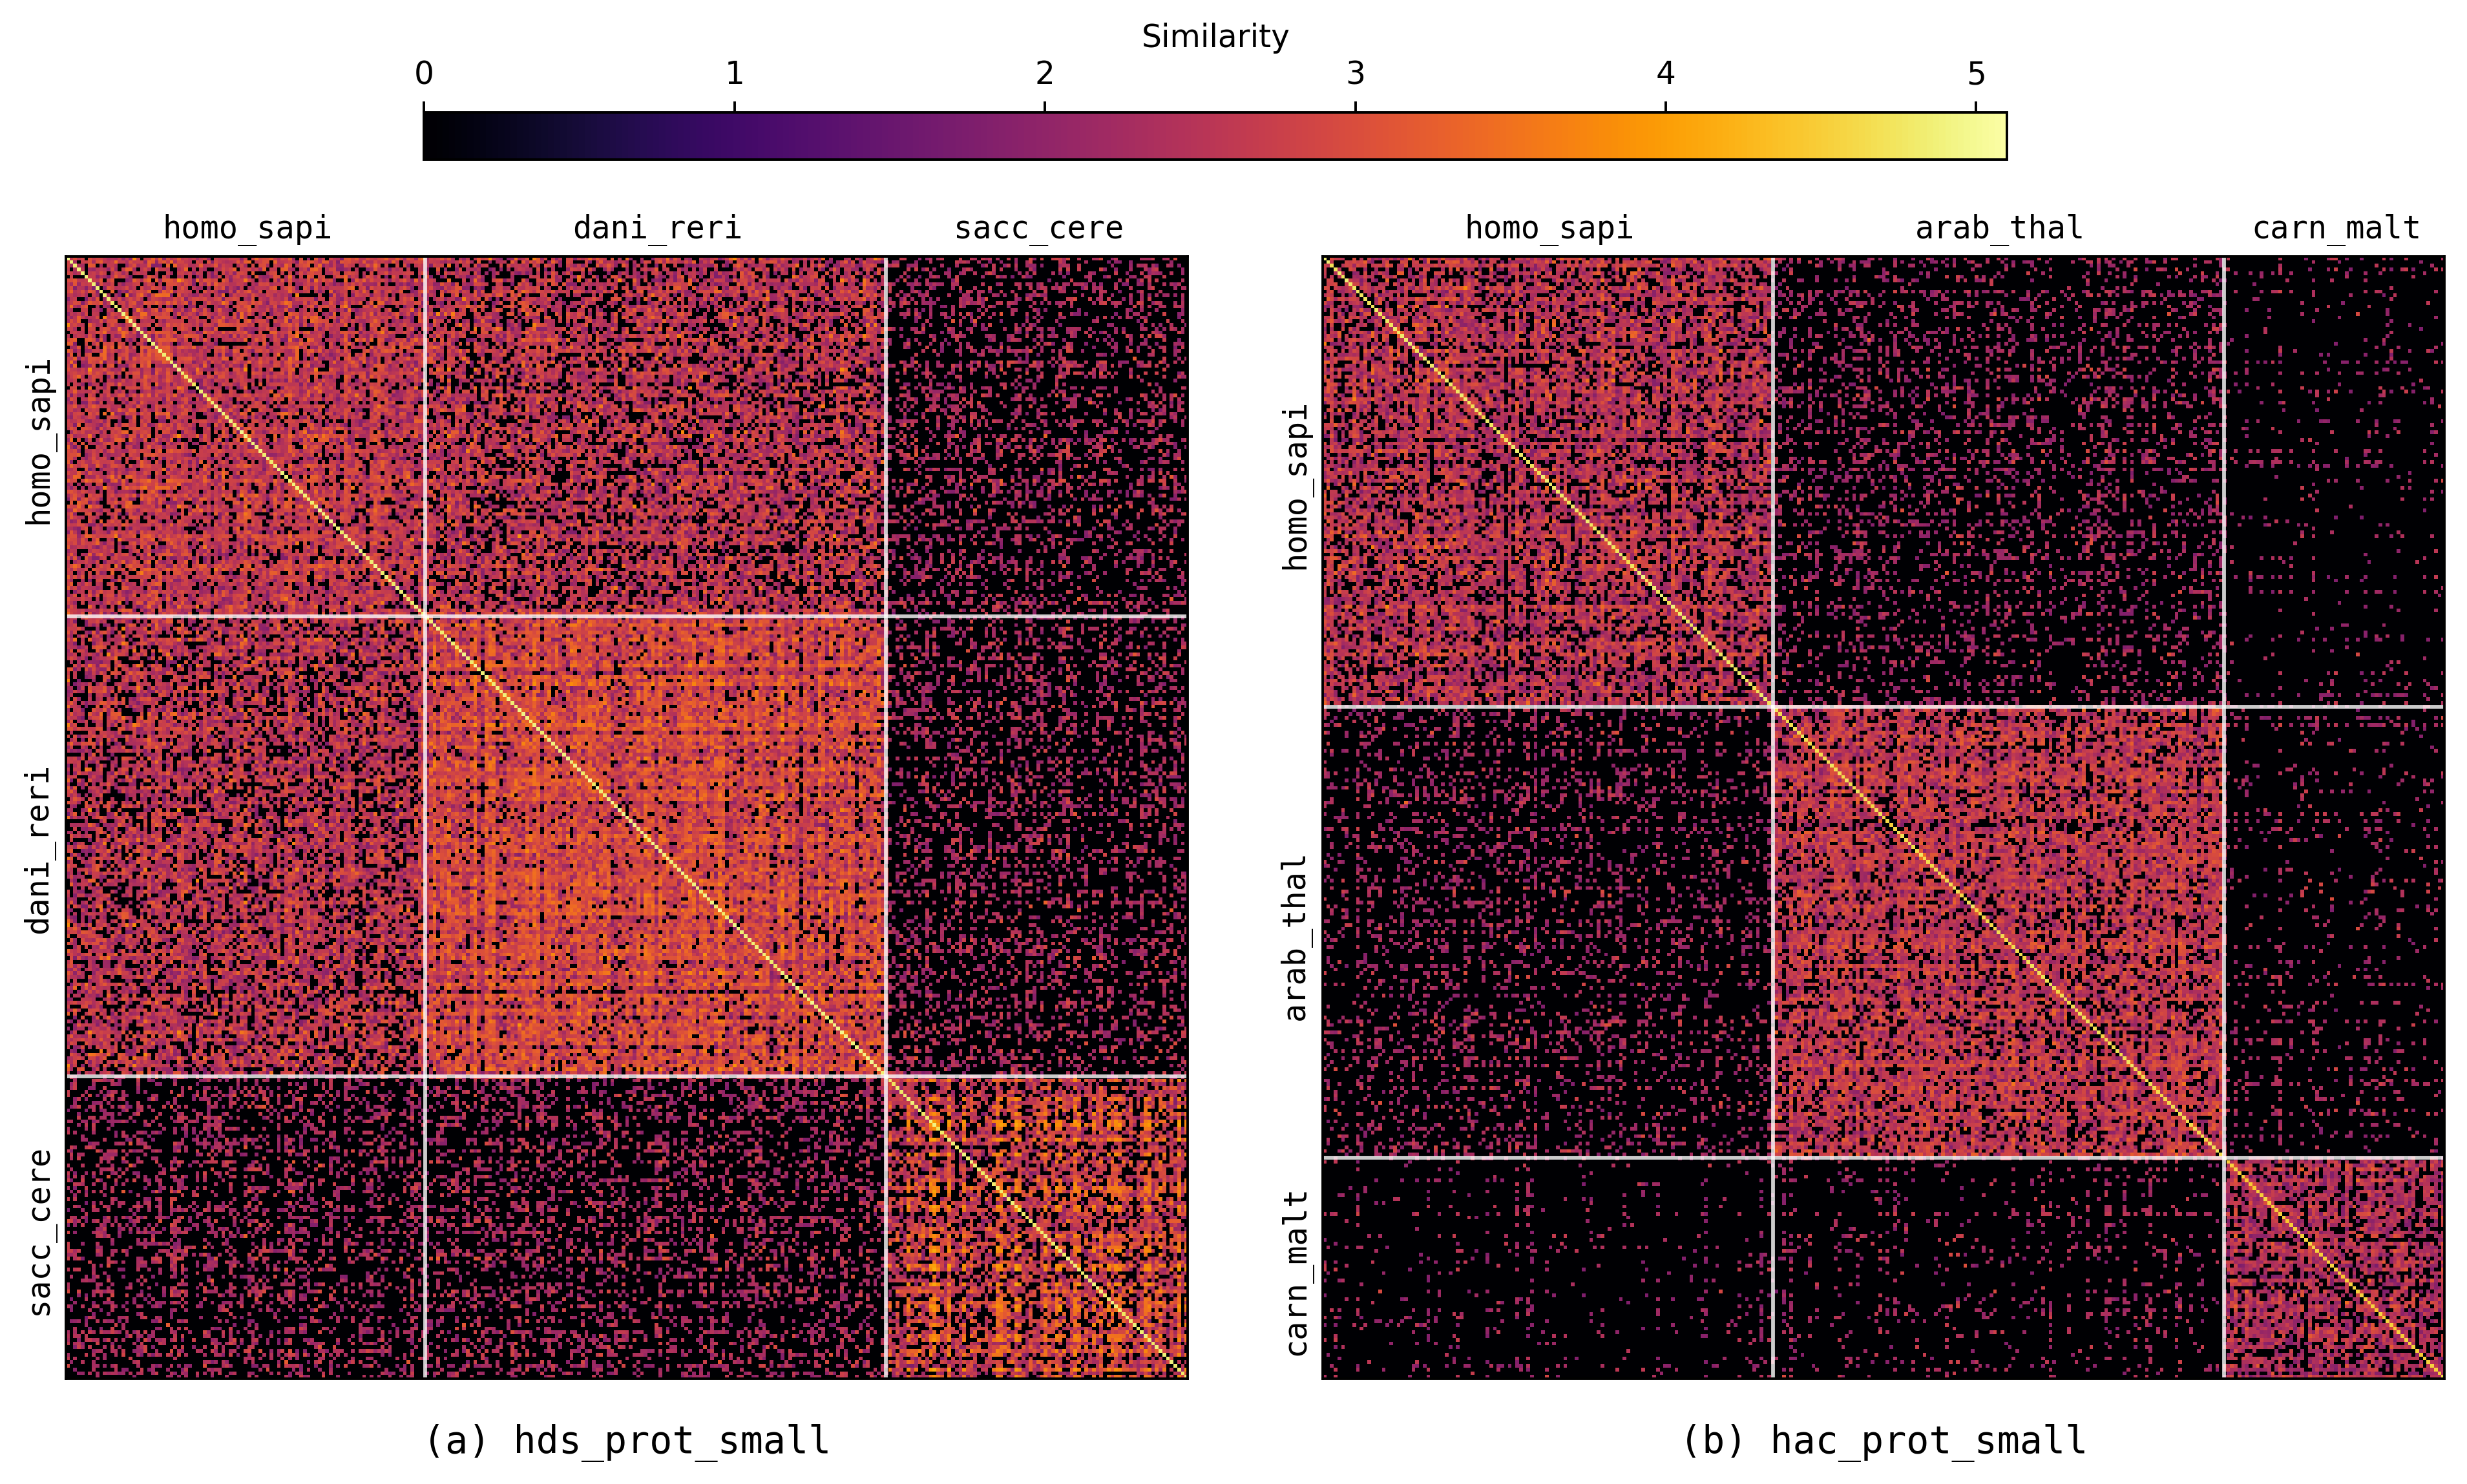
\includegraphics[width=1\linewidth]{asset/adj_hds_hac.png}
  \caption{Heatmap of bin-aggregated adjacency matrices for two PSSN datasets.
  Color intensity reflects logarithmically scaled summed BLASTp similarity (bit
  score) between bins of vertices. White lines separate organism-specific
  partitions. For the \texttt{hds\_prot\_small} dataset (a): \textit{Homo sapiens}
  (human), \textit{Danio rerio} (zebrafish), and \textit{Saccharomyces
  cerevisiae} (fungus). For the \texttt{hac\_prot\_small} dataset (b): \textit{Homo
  sapiens} (human), \textit{Arabidopsis thaliana} (plant), and
  \textit{Carnobacterium maltaromaticum} (bacterium).}
  \label{fig:res}
\end{figure}

\begin{figure}[htbp]
  \begin{adjustwidth}{-1.2cm}{-1.2cm}
    \centering

    \begin{subfigure}{0.49\linewidth}
      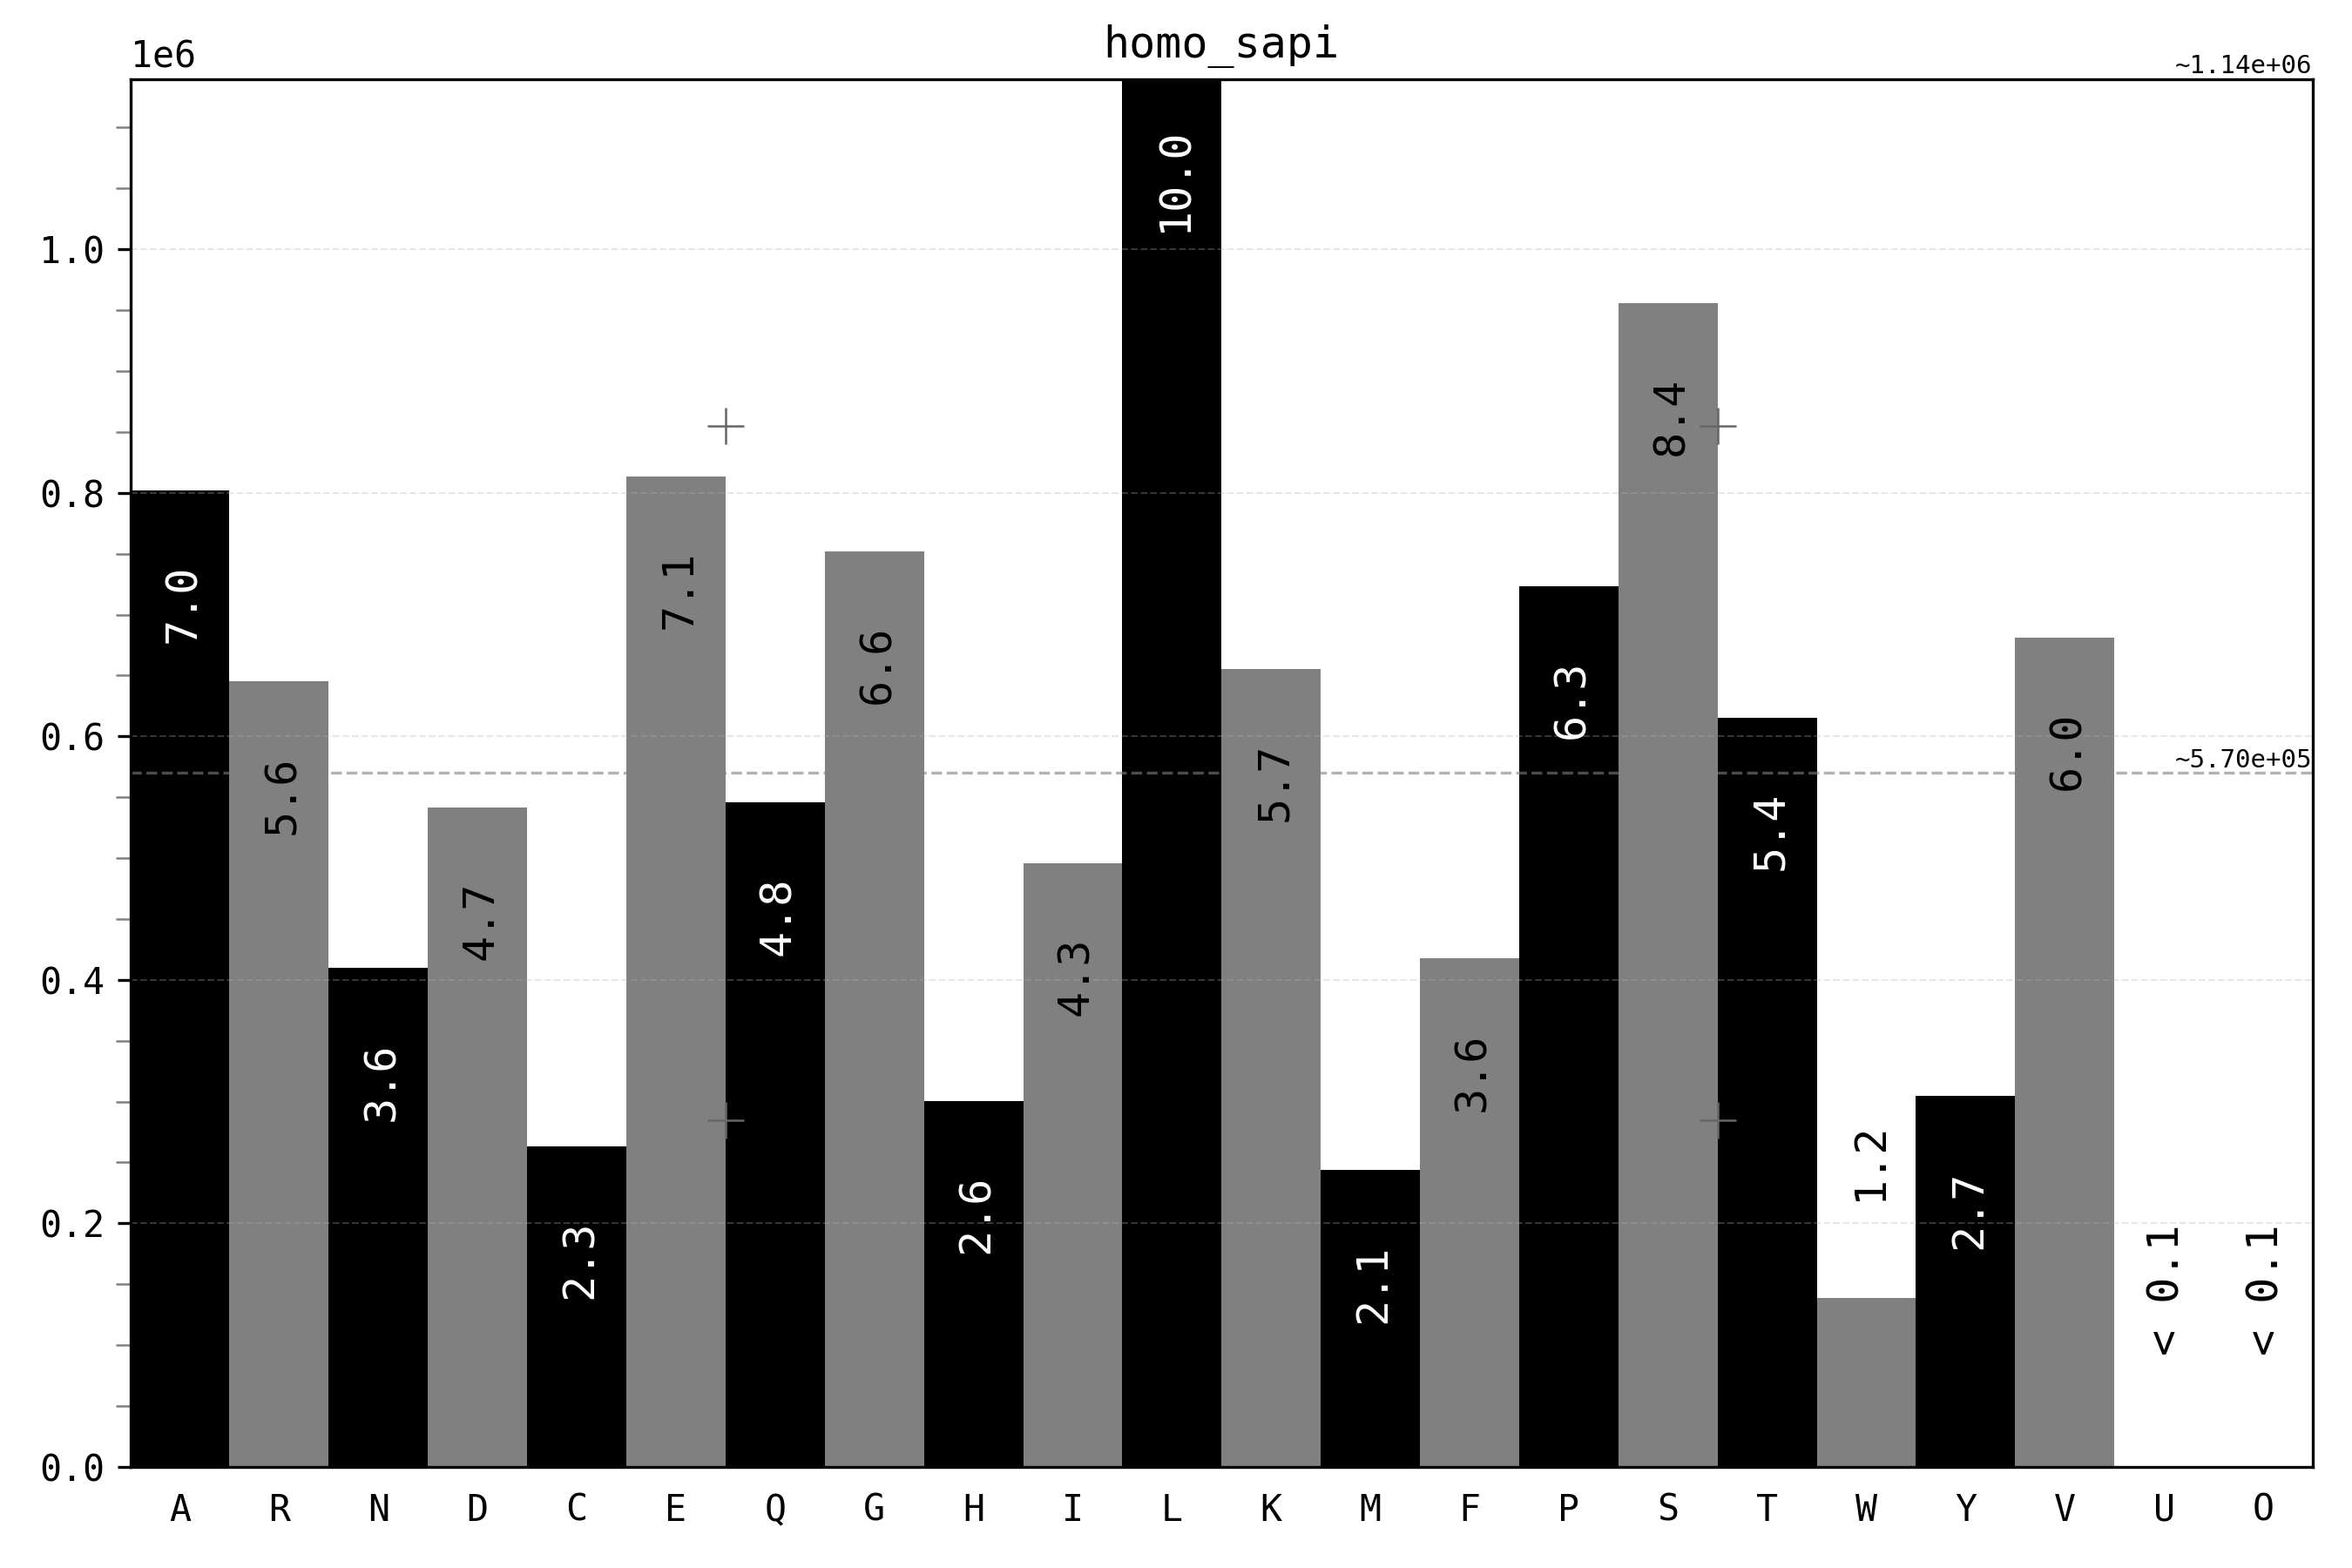
\includegraphics[width=\linewidth]{asset/aa_distr_homo_sapi.png}
      \subcaption{\textit{Homo sapiens} (human) reference proteome. Composition: 20,647 protein sequences.}
      \label{fig:aa_distr_homo_sapi}
    \end{subfigure}

    \vspace{0.4cm}

    \begin{subfigure}{0.49\linewidth}
      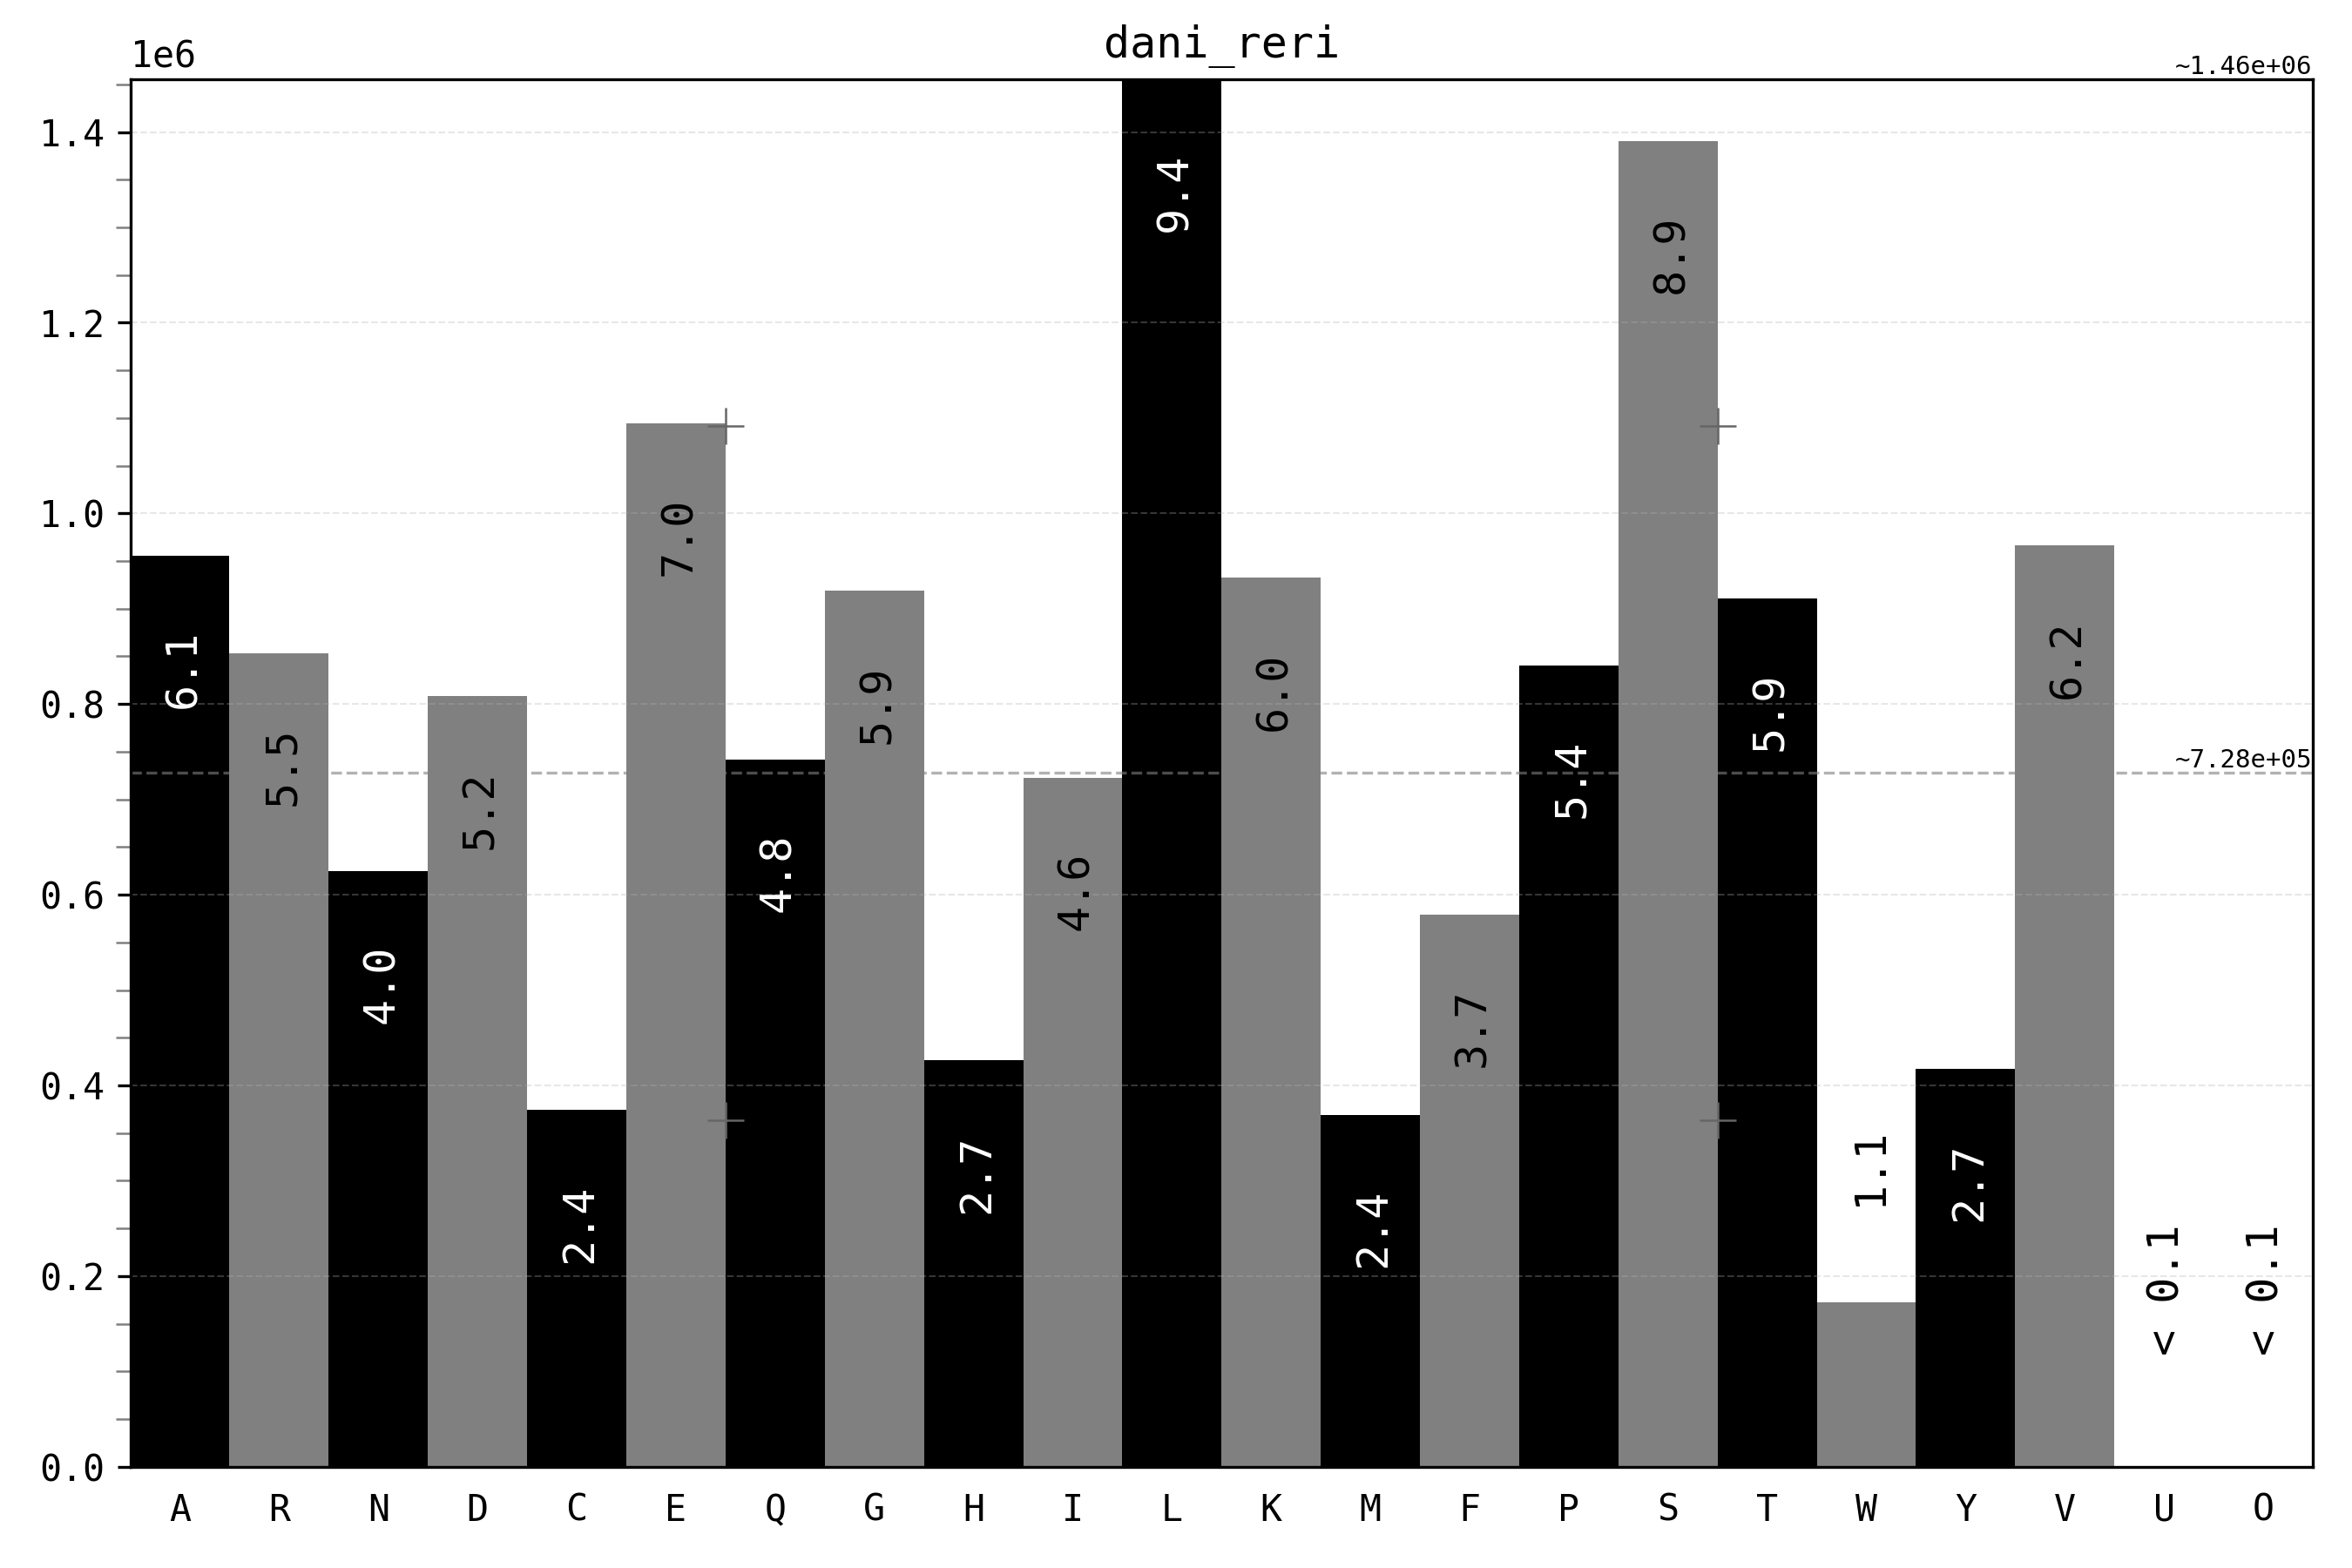
\includegraphics[width=\linewidth]{asset/aa_distr_dani_reri.png}
      \subcaption{\textit{Danio rerio} (zebrafish) reference proteome. Composition: 26,728 protein sequences.}
      \label{fig:aa_distr_dani_reri}
    \end{subfigure}
    \hfill
    \begin{subfigure}{0.49\linewidth}
      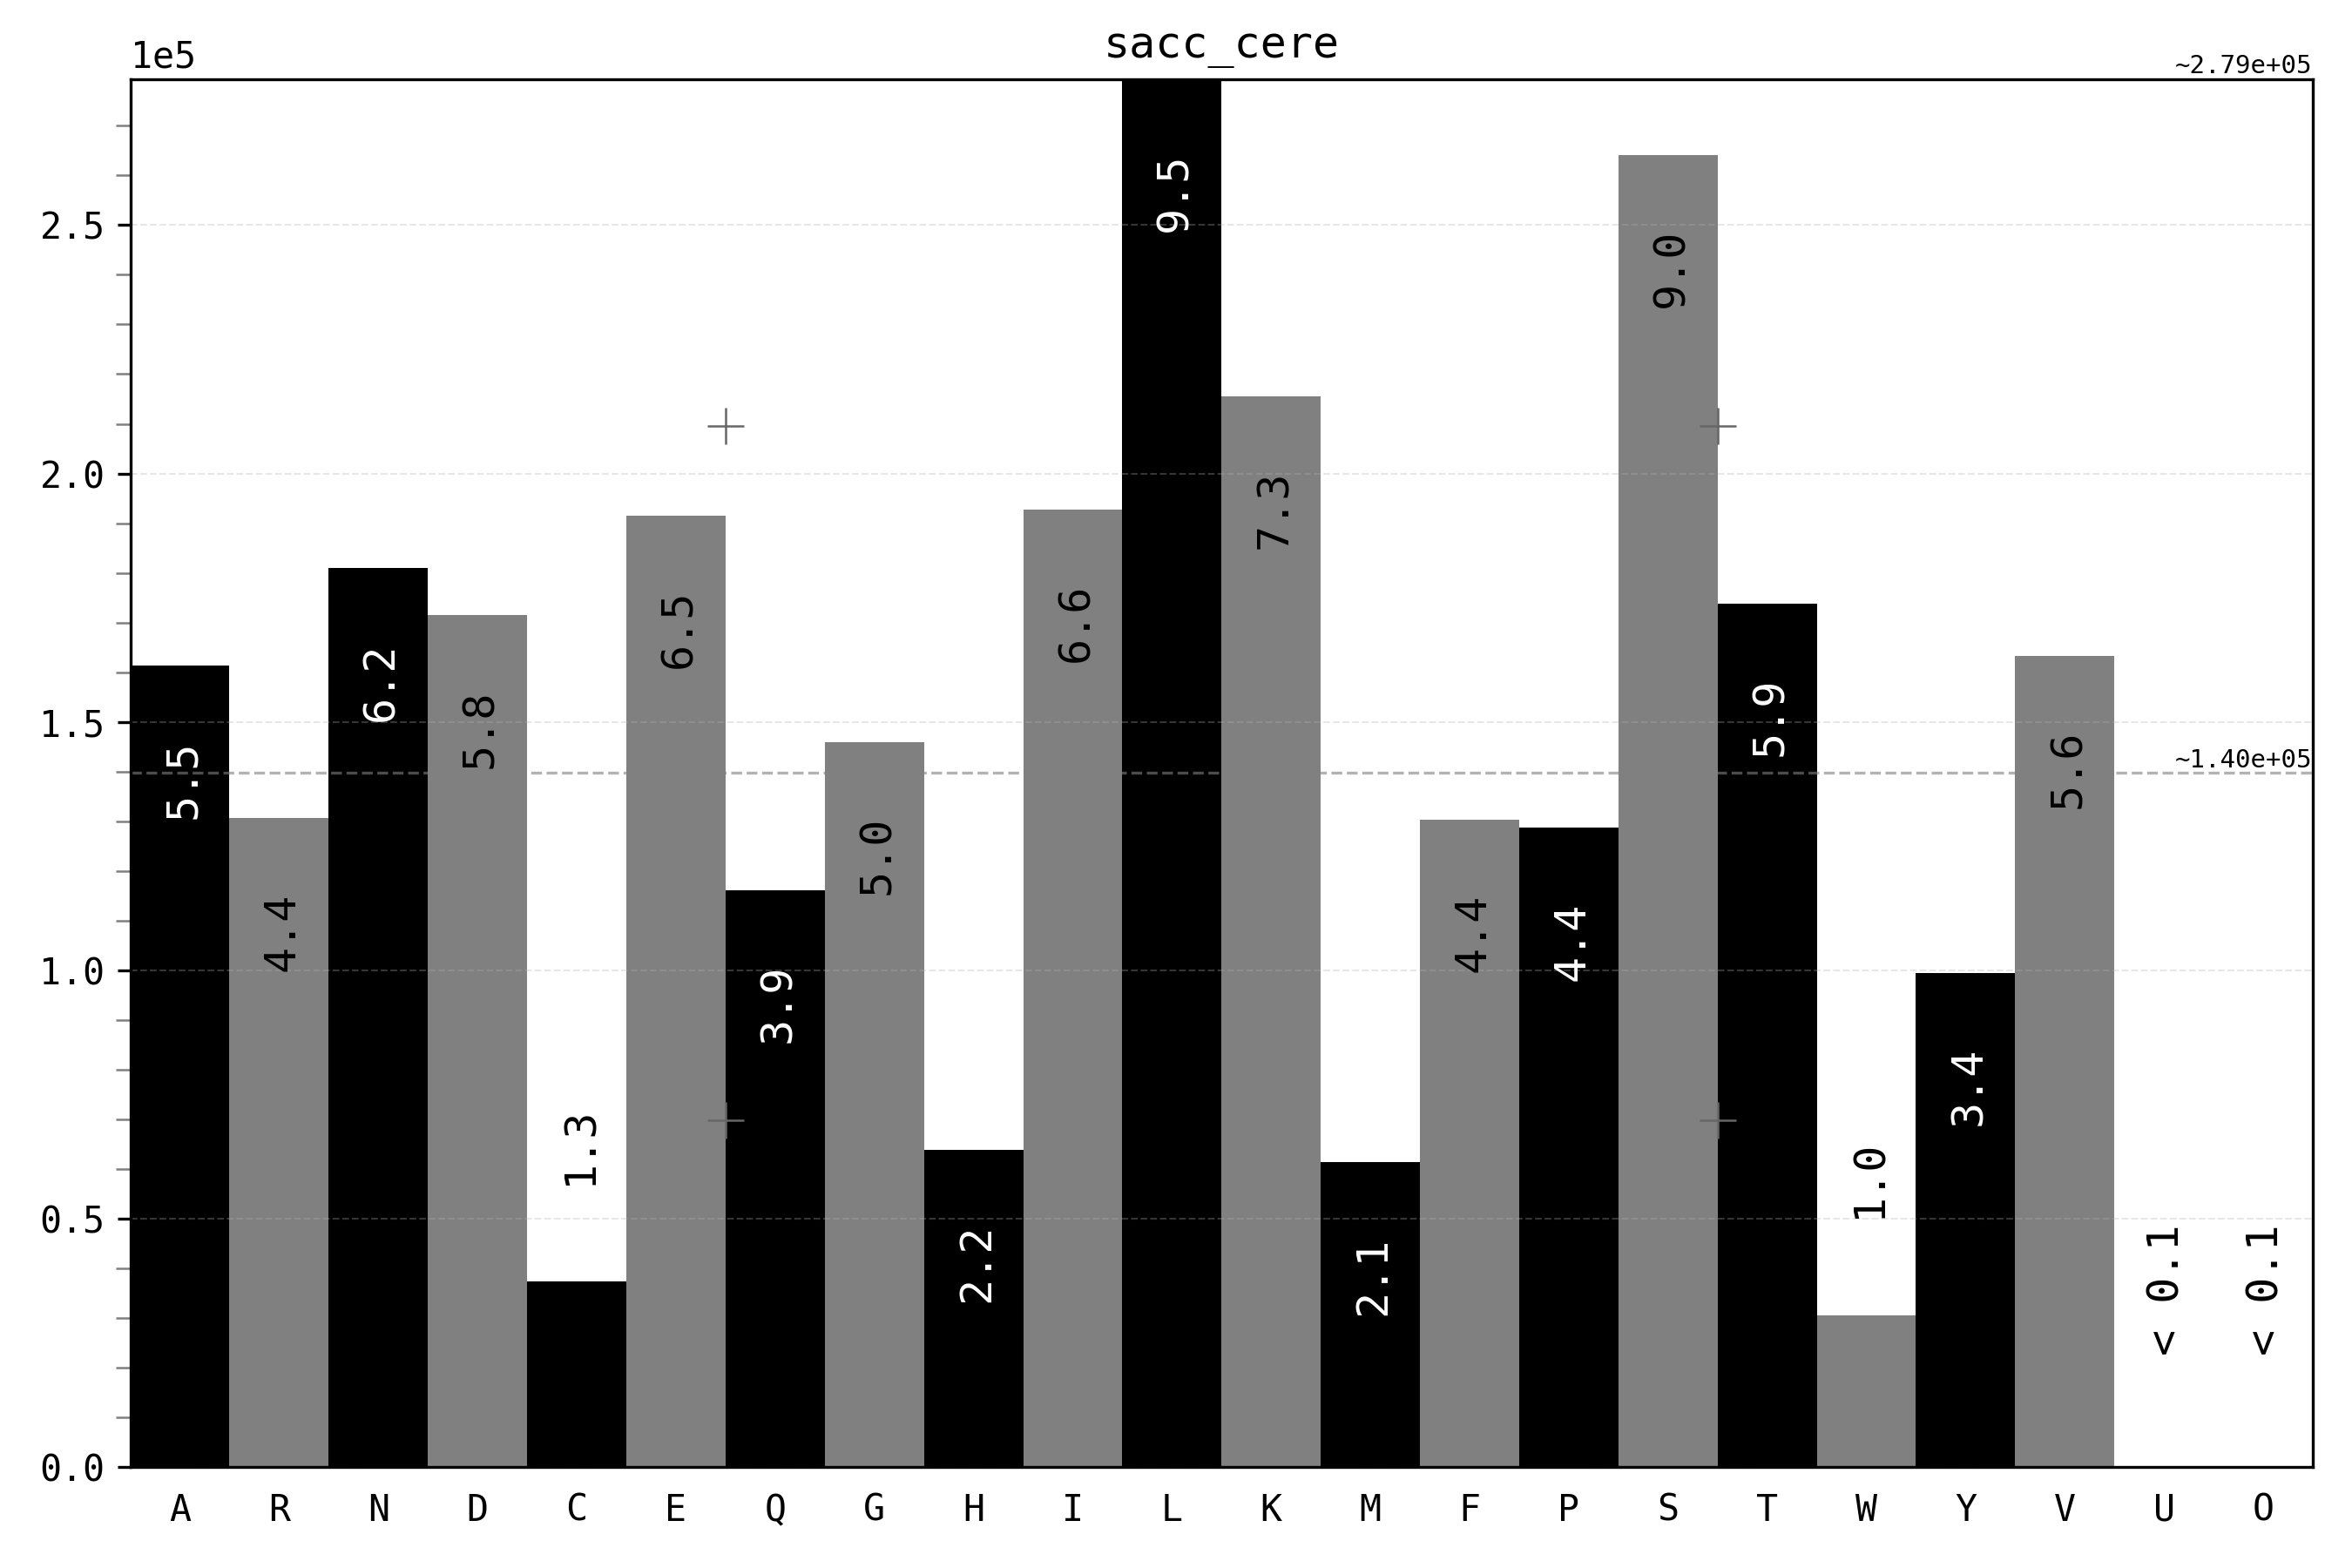
\includegraphics[width=\linewidth]{asset/aa_distr_sacc_cere.png}
      \subcaption{\textit{Saccharomyces cerevisiae} (fungus) reference proteome. Composition: 6,065 protein sequences.}
      \label{fig:aa_distr_sacc_cere}
    \end{subfigure}

    \vspace{0.4cm}

    \begin{subfigure}{0.49\linewidth}
      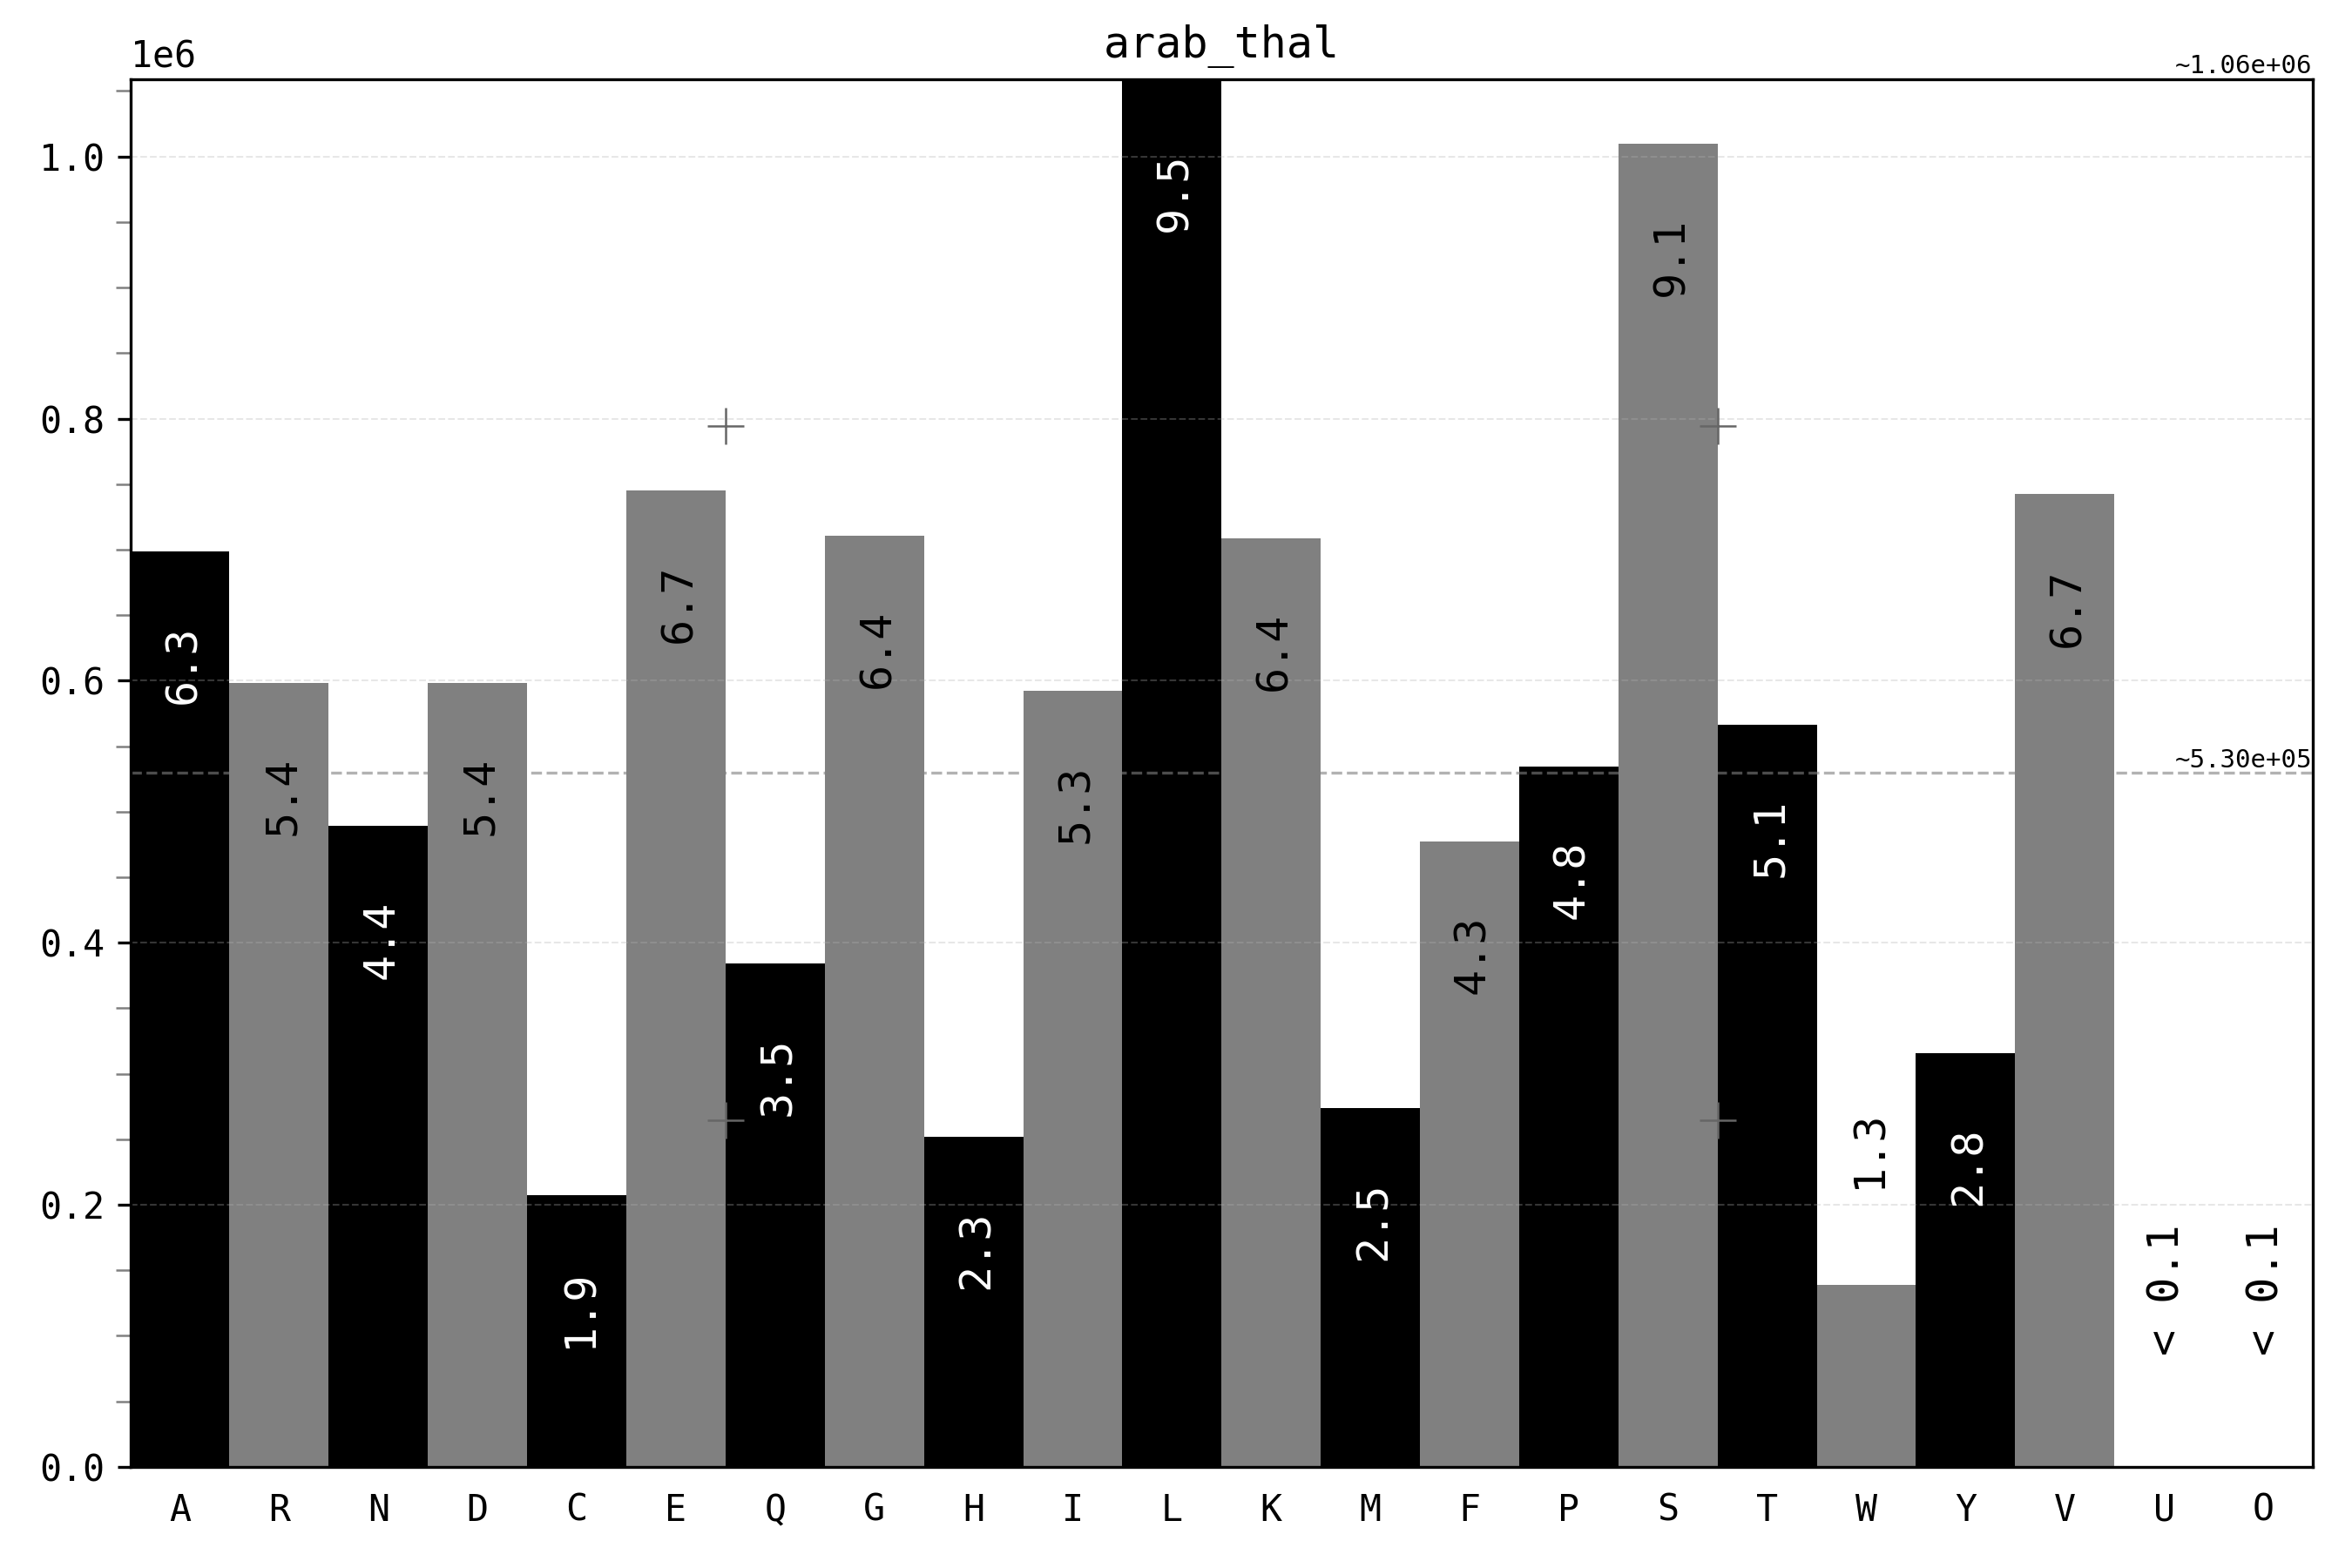
\includegraphics[width=\linewidth]{asset/aa_distr_arab_thal.png}
      \subcaption{\textit{Arabidopsis thaliana} (plant) reference proteome. Composition: 27,448 protein sequences.}
      \label{fig:aa_distr_arab_thal}
    \end{subfigure}
    \hfill
    \begin{subfigure}{0.49\linewidth}
      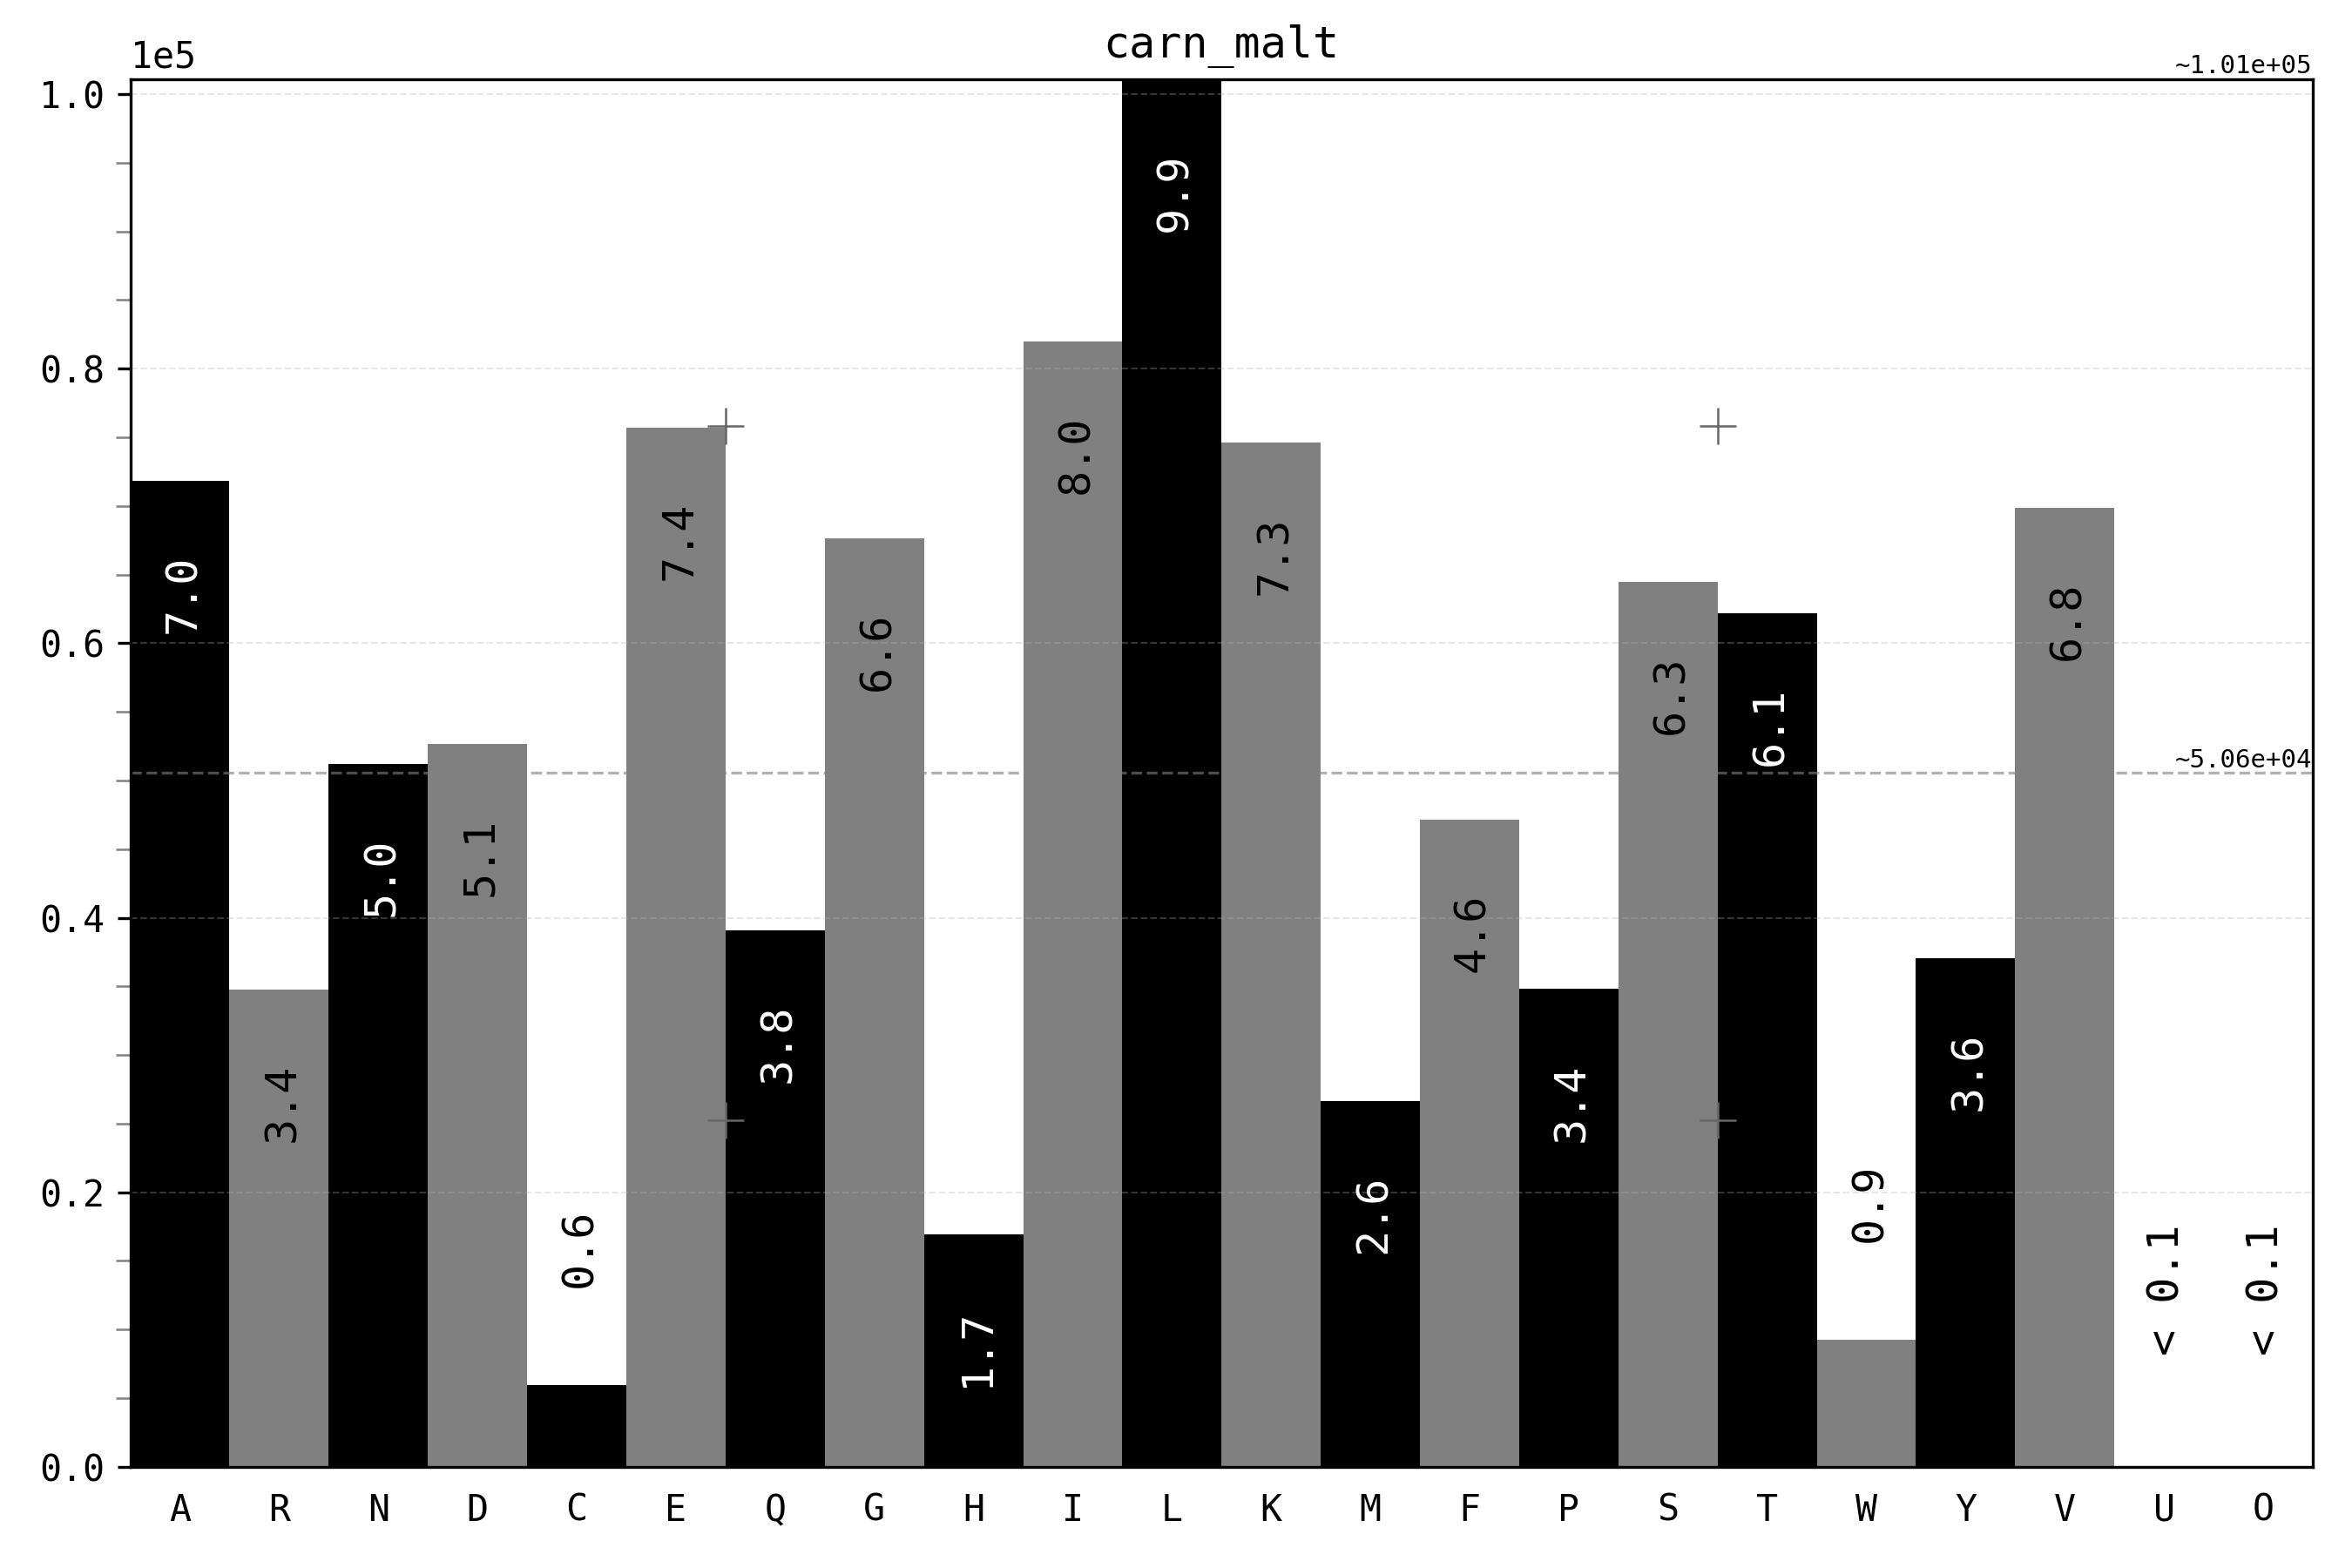
\includegraphics[width=\linewidth]{asset/aa_distr_carn_malt.png}
      \subcaption{\textit{Carnobacterium maltaromaticum} (bacterium) reference proteome. Composition: 3,539 protein sequences.}
      \label{fig:aa_distr_carn_malt}
    \end{subfigure}

    \caption{Distribution of residues per amino acid type for a selected
    collection of datasets (refer to Table~\ref{tab:dataStats}). The vertical
    axis shows the count of residues; bar heights are proportional to the
    amount of residues that correspond to that amino acid from the associated
    dataset after all sequences are concatenated. Each label displays the
    fraction (\%) of residues for that amino acid.}
    \label{fig:aa_distr}
  \end{adjustwidth}
\end{figure}

\begin{figure}[htbp]
  \begin{adjustwidth}{0cm}{0cm}
    \centering
    \begin{subfigure}{\linewidth}
      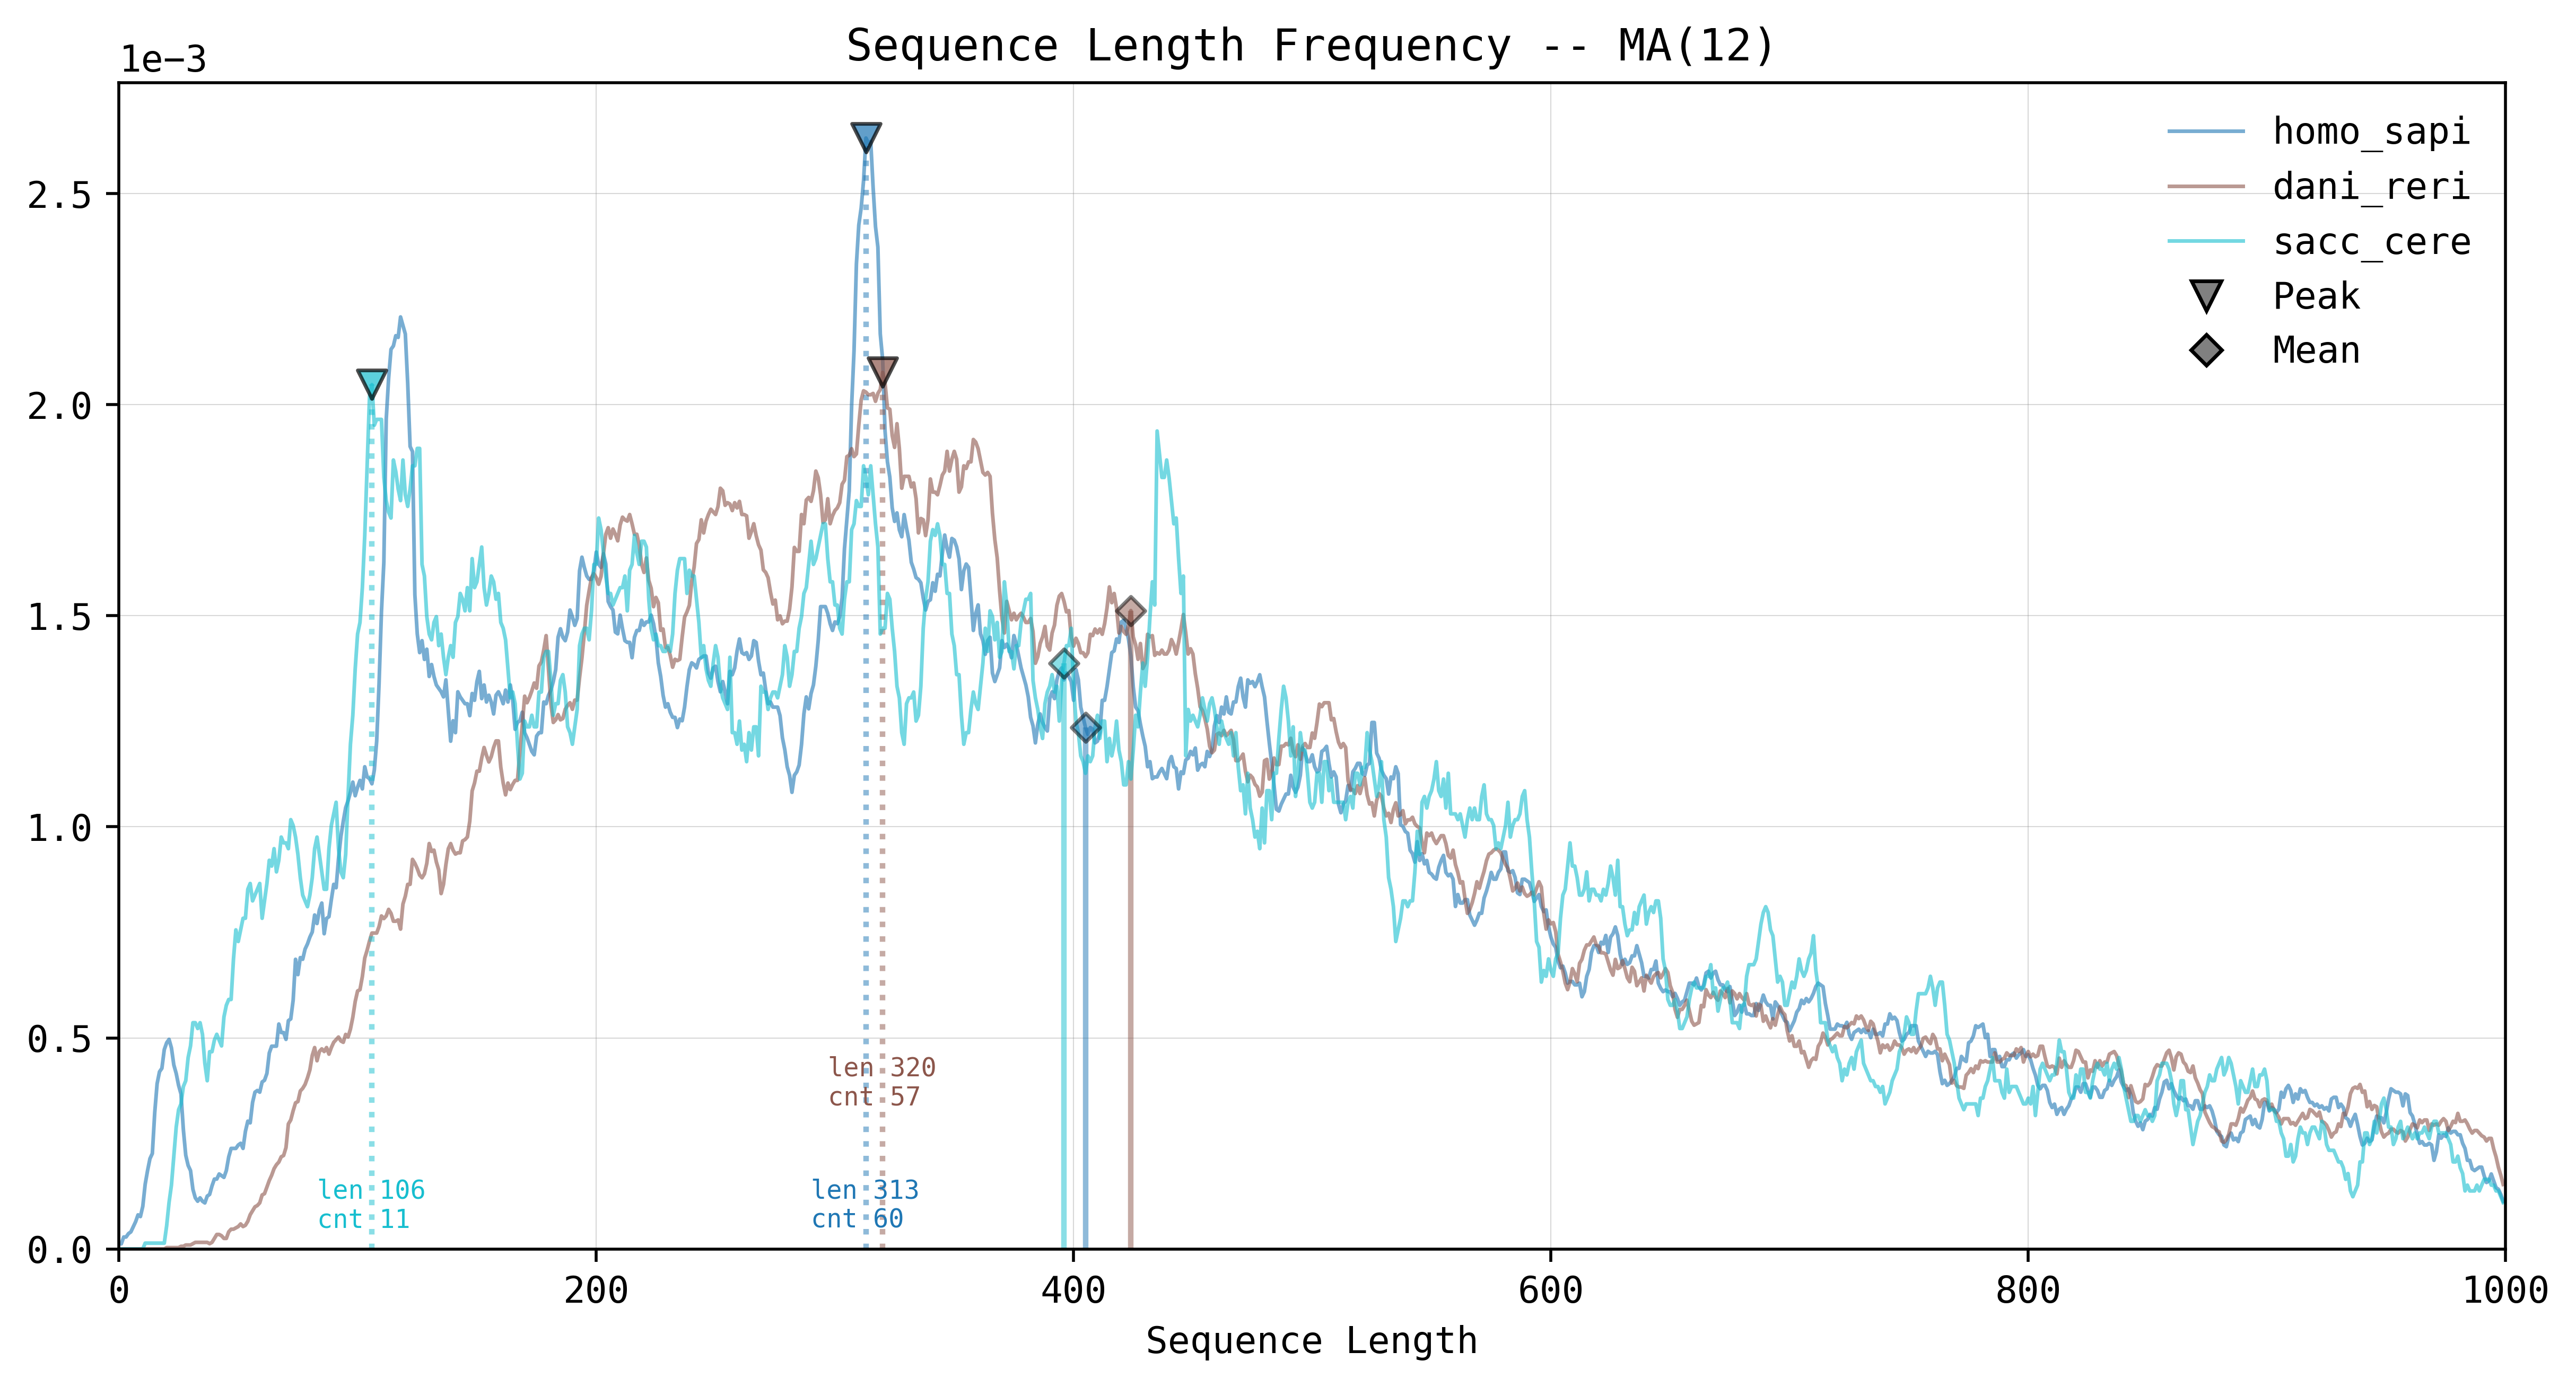
\includegraphics[width=1\linewidth]{asset/len_freq_hds.png}
      \subcaption{\texttt{hds\_prot}: \textit{H. sapiens}, \textit{D. rerio}
      and \textit{S. cerevisiae} with peak lengths 313, 320, and 106 residues,
      occurring 60, 57, and 11 times respectively.}
      \label{fig:len_freq_hds}
    \end{subfigure}
    \\[0.5cm]
    \begin{subfigure}{\linewidth}
      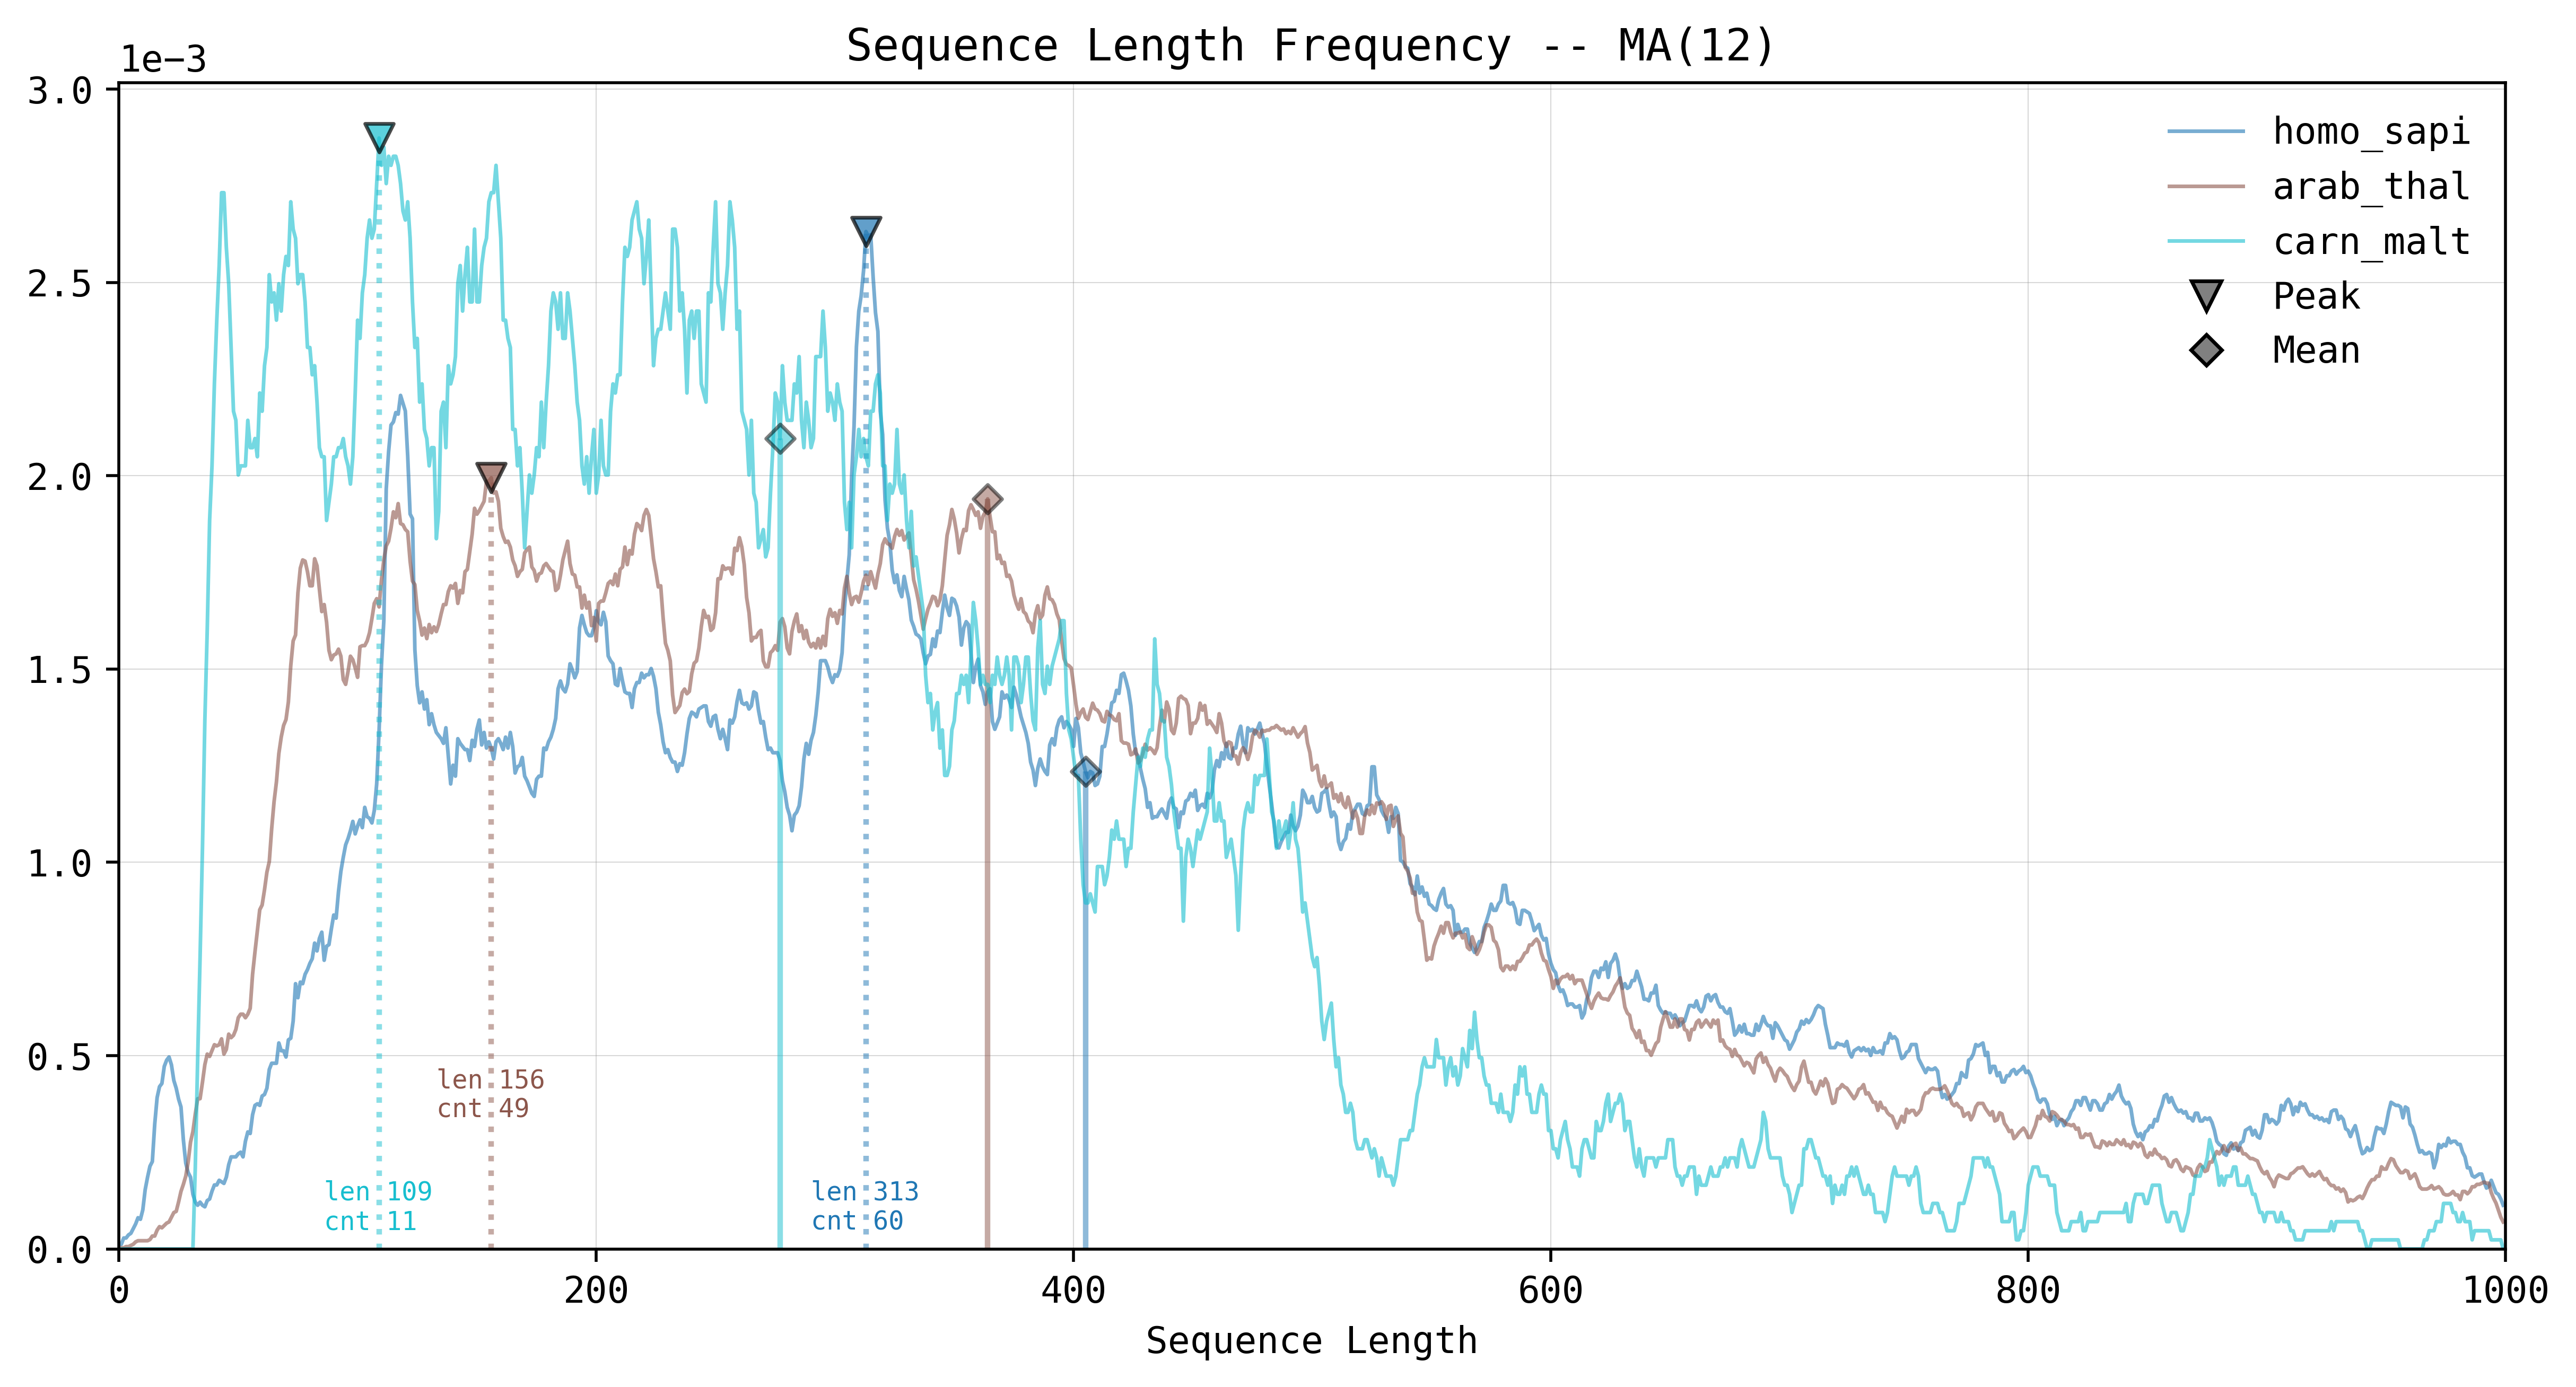
\includegraphics[width=1\linewidth]{asset/len_freq_hac.png}
      \subcaption{\texttt{hac\_prot}: \textit{H. sapiens}, \textit{A. thaliana}
      and \textit{C. maltaromaticum} with peak lengths 313, 156, and 109
      residues, occurring 60, 49, and 11 times respectively.}
      \label{fig:len_freq_hac}
    \end{subfigure}
  \end{adjustwidth}
  \vspace{0.0cm}
  \caption{Smoothed sequence length distributions for \texttt{hds\_prot} (top)
  and \texttt{hac\_prot} (bottom). A moving average with window size 12 was
  applied to the normalized frequency counts. Peak ($\blacktriangledown$) and
  mean ($\blacklozenge$) are annotated. Lengths shown up to 1000 residues.}
  \label{fig:len_freq}
\end{figure}

\begin{figure}[htbp]
  \vspace{-0.5cm}
  \begin{adjustwidth}{-0cm}{-0cm}
    \centering

    \begin{subfigure}{0.44\linewidth}
      \fcolorbox{lightgray}{white}{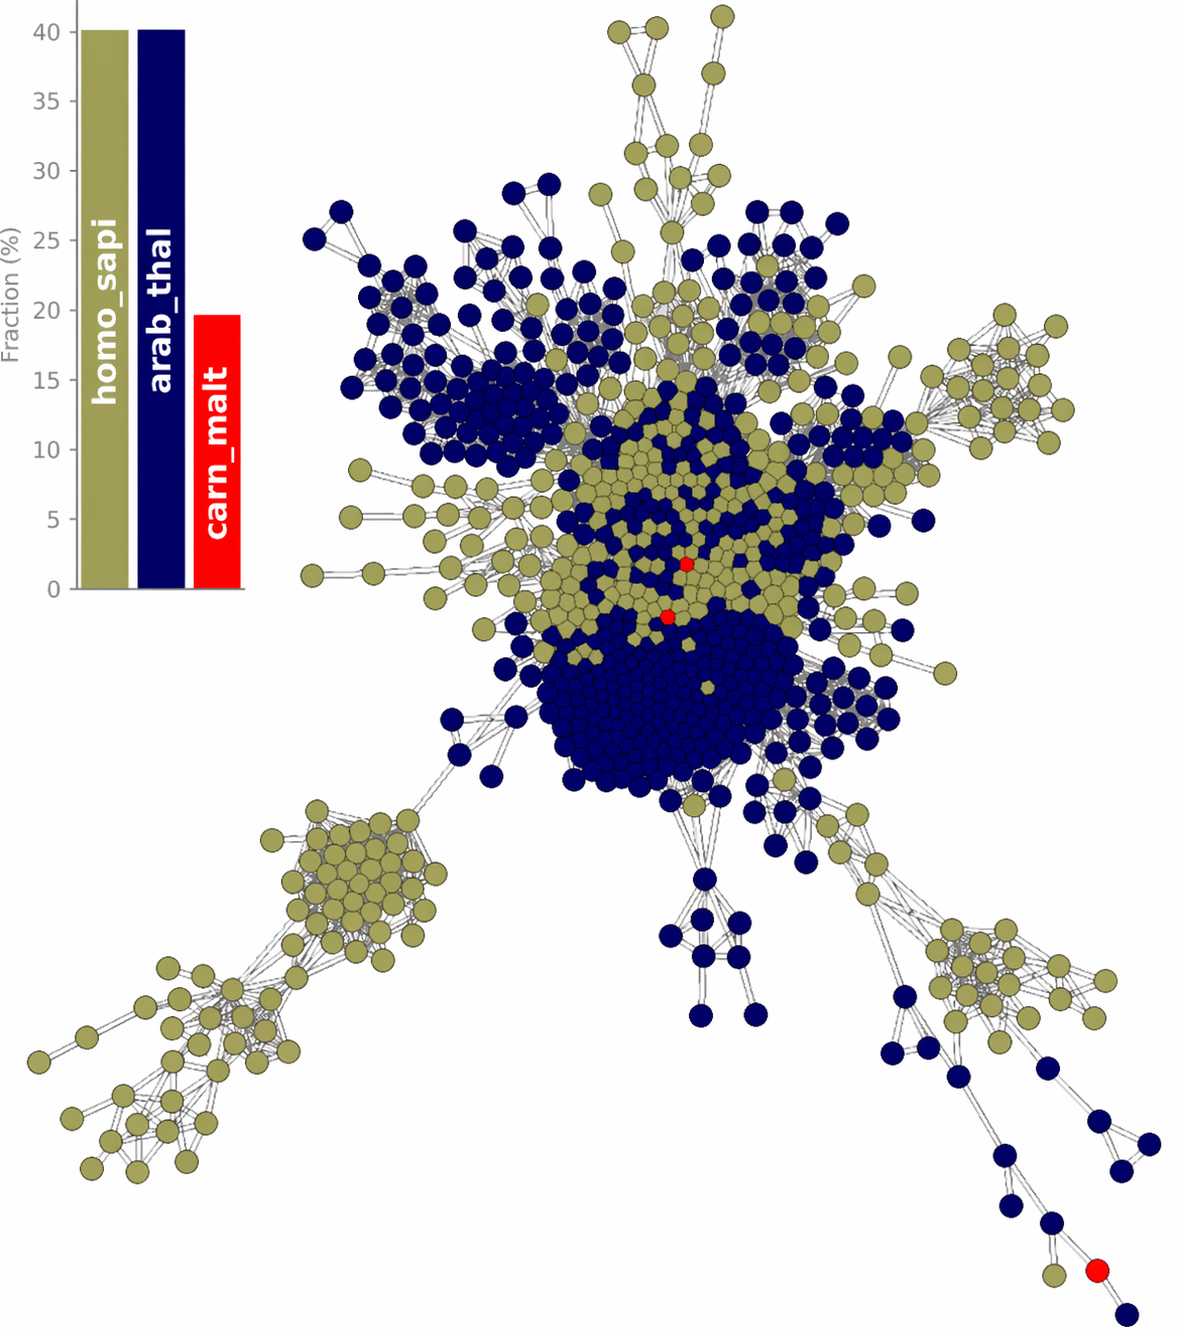
\includegraphics[width=\linewidth]{asset/graph_hac_small_taxid.png}}
      \subcaption{Taxonomic classification of the dataset
      \texttt{hac\_prot\_small}. Each color group corresponds to a unique
      composite proteome.}
      \label{fig:graph_hac_small_taxid}
    \end{subfigure}
    \hspace{0.5cm}
    \begin{subfigure}{0.44\linewidth}
      \fcolorbox{lightgray}{white}{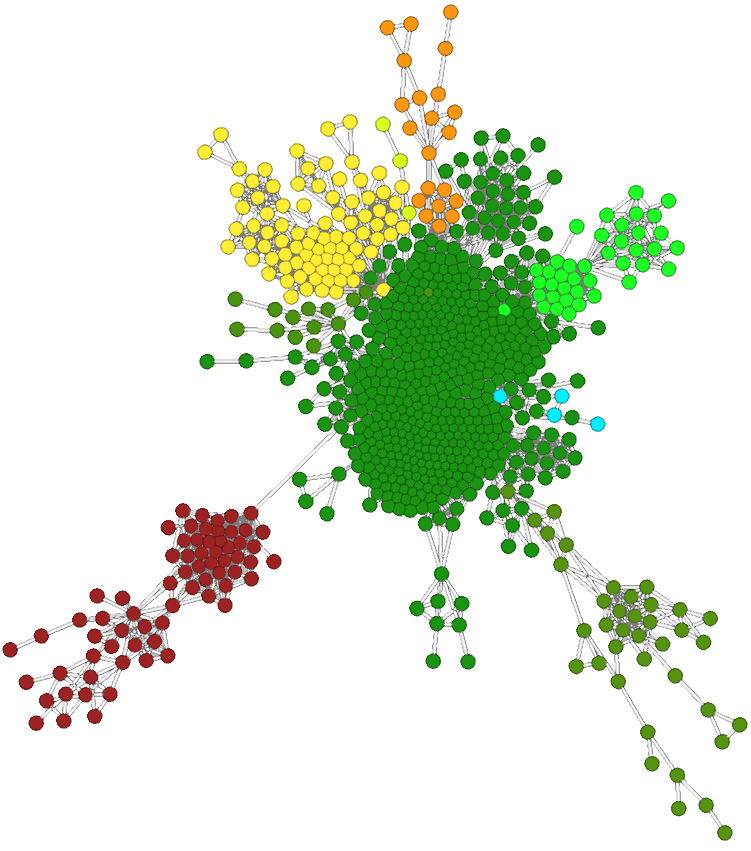
\includegraphics[width=\linewidth]{asset/graph_hac_small_mcl_1_2.png}}
      \subcaption{MCL partitioning of the dataset \texttt{hac\_prot\_small}.
      Each color group is a unique protein community.}
      \label{fig:graph_hac_small_mcl_1_2}
    \end{subfigure}

    \vspace{0.4cm}

    \begin{subfigure}{0.44\linewidth}
      \fcolorbox{lightgray}{white}{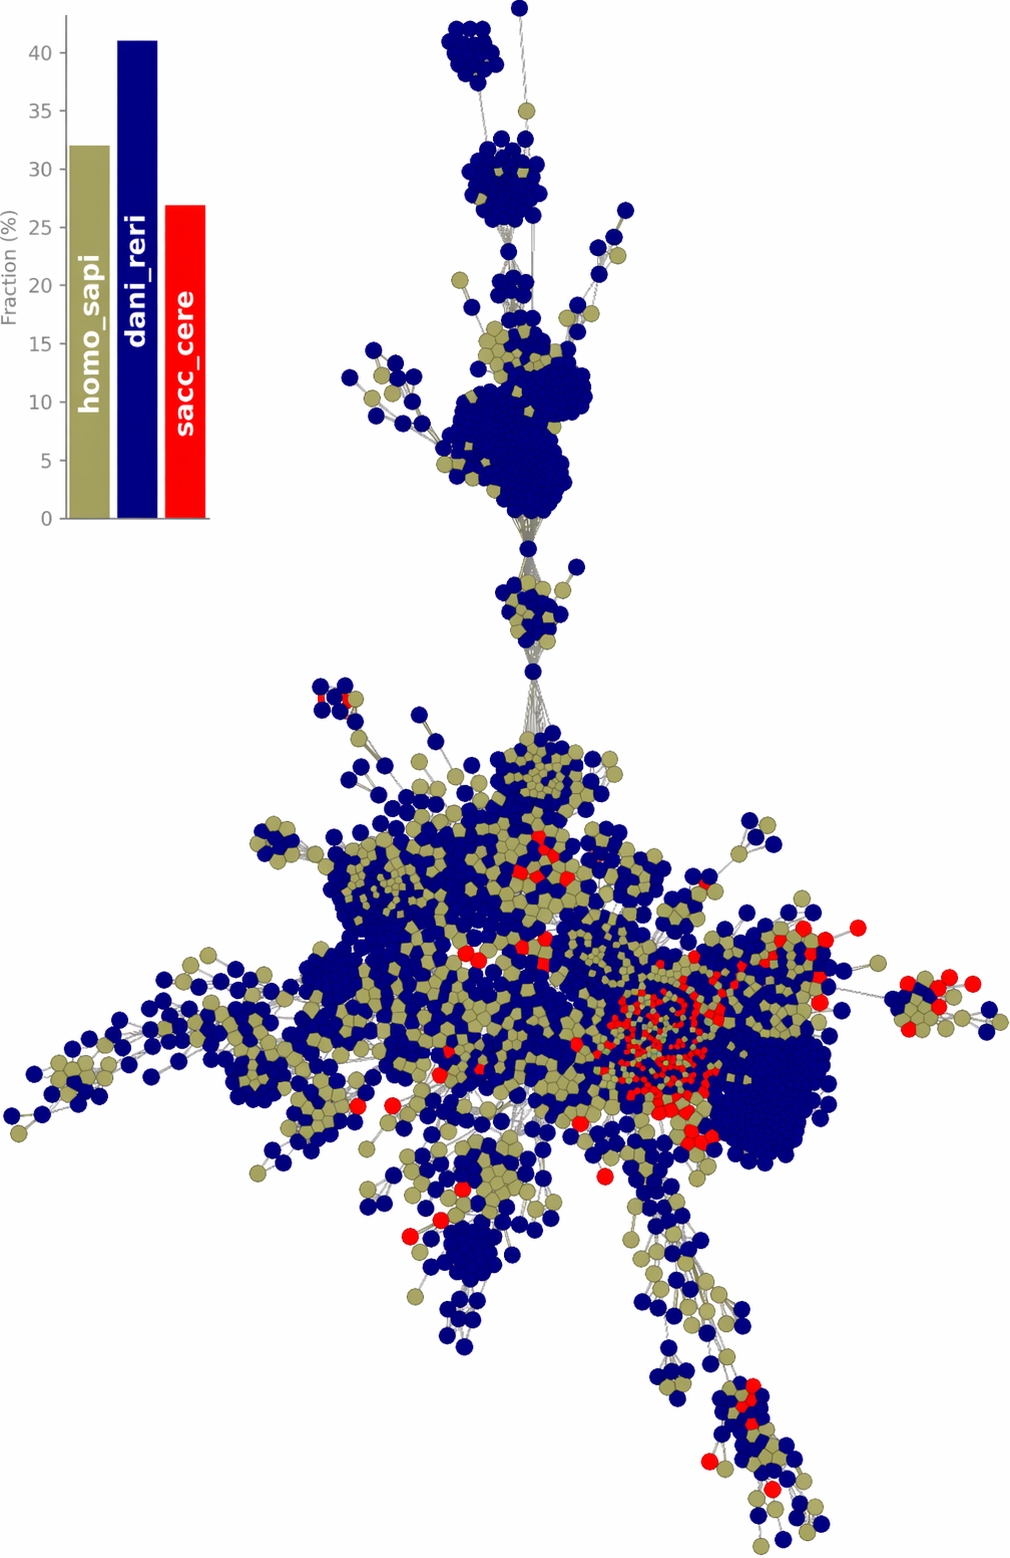
\includegraphics[width=\linewidth]{asset/graph_hds_small_taxid.png}}
      \subcaption{Taxonomic classification of the dataset
      \texttt{hds\_prot\_small}. Each color group corresponds to a unique
      composite proteome.}
      \label{fig:graph_hds_small_taxid}
    \end{subfigure}
    \hspace{0.5cm}
    \begin{subfigure}{0.44\linewidth}
      \fcolorbox{lightgray}{white}{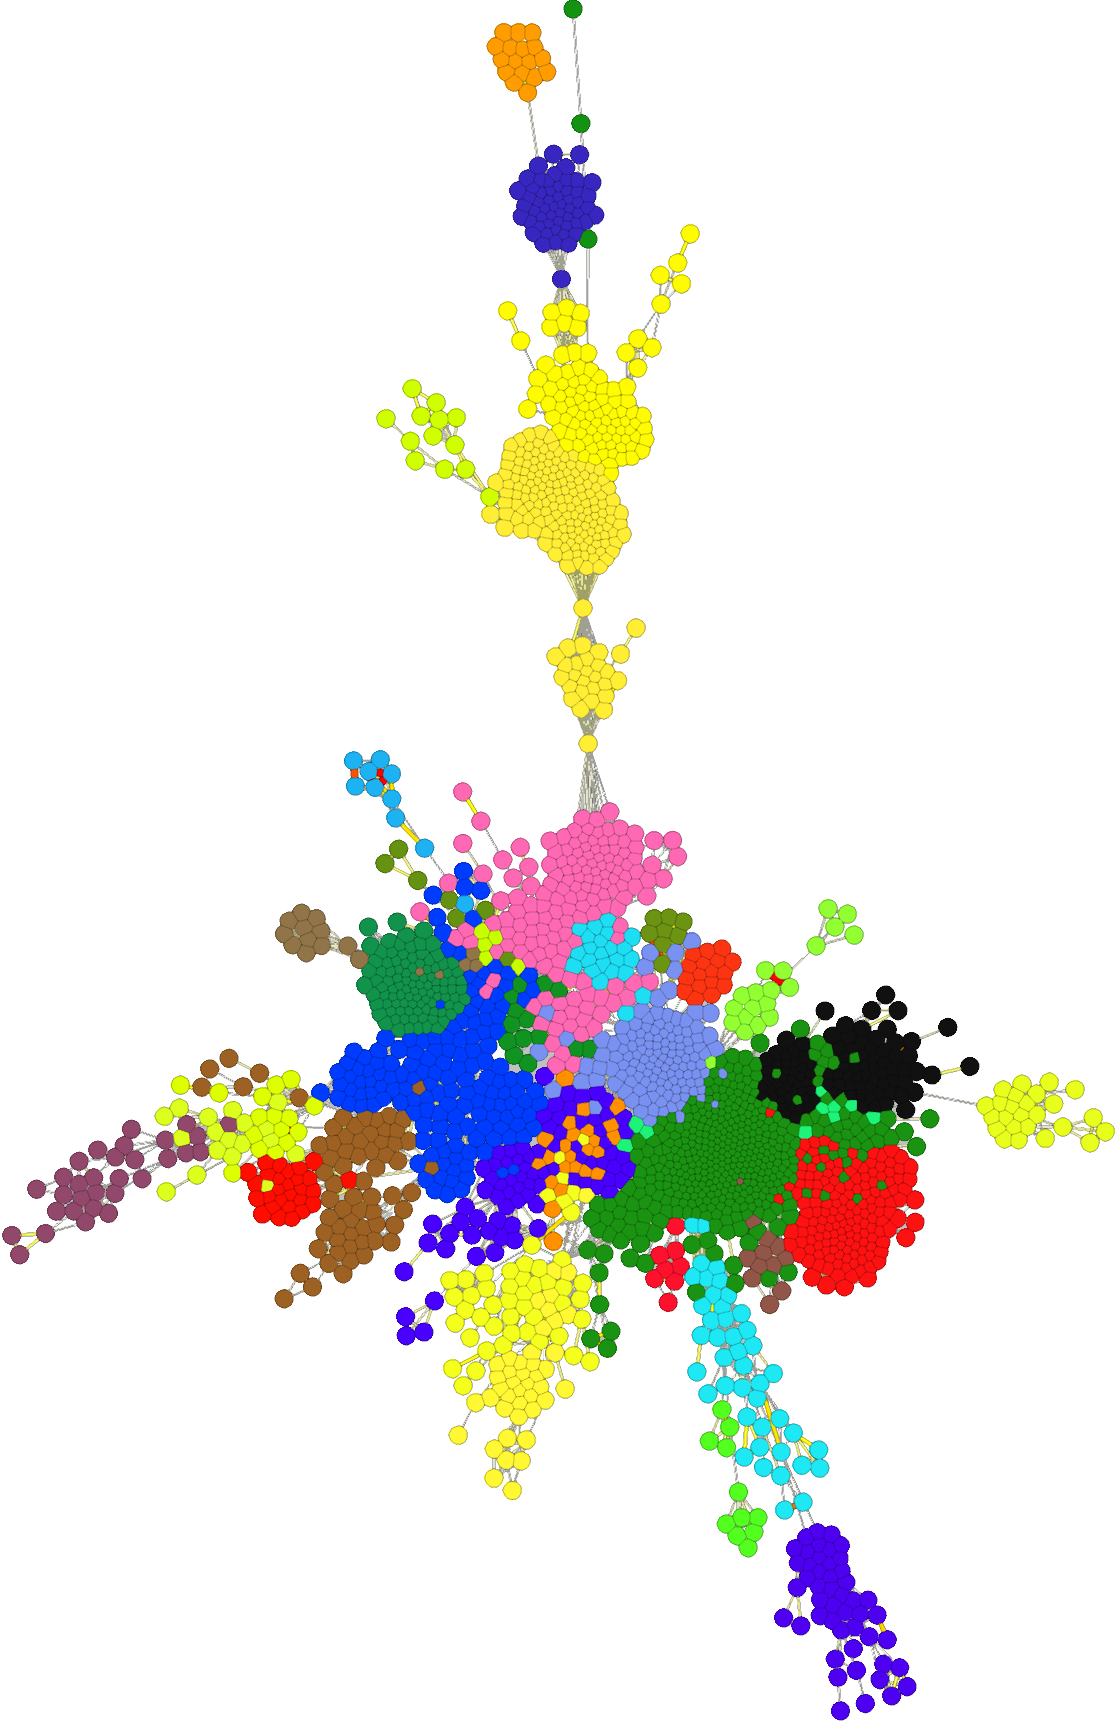
\includegraphics[width=\linewidth]{asset/graph_hds_small_mcl_1_2.png}}
      \subcaption{MCL partitioning of the dataset \texttt{hds\_prot\_small}.
      Each color group is a unique protein community.}
      \label{fig:graph_hds_small_mcl_1_2}
    \end{subfigure}

    \vspace{0.1cm}

    \caption{Graph visualization of two hybrid datasets. Edges indicate
    statistically significant similarity for vertex pairs. Comparison of
    TaxID-based coloring on the left and MCL-based coloring on the right with
    inflation parameter 1.2. Shown are the largest connected subgraphs. The
    tool used to perform this visualization is Graphia \cite{graphia}.}

    \label{fig:graph}
  \end{adjustwidth}
\end{figure}

\begin{figure}[htbp]
  \centering
  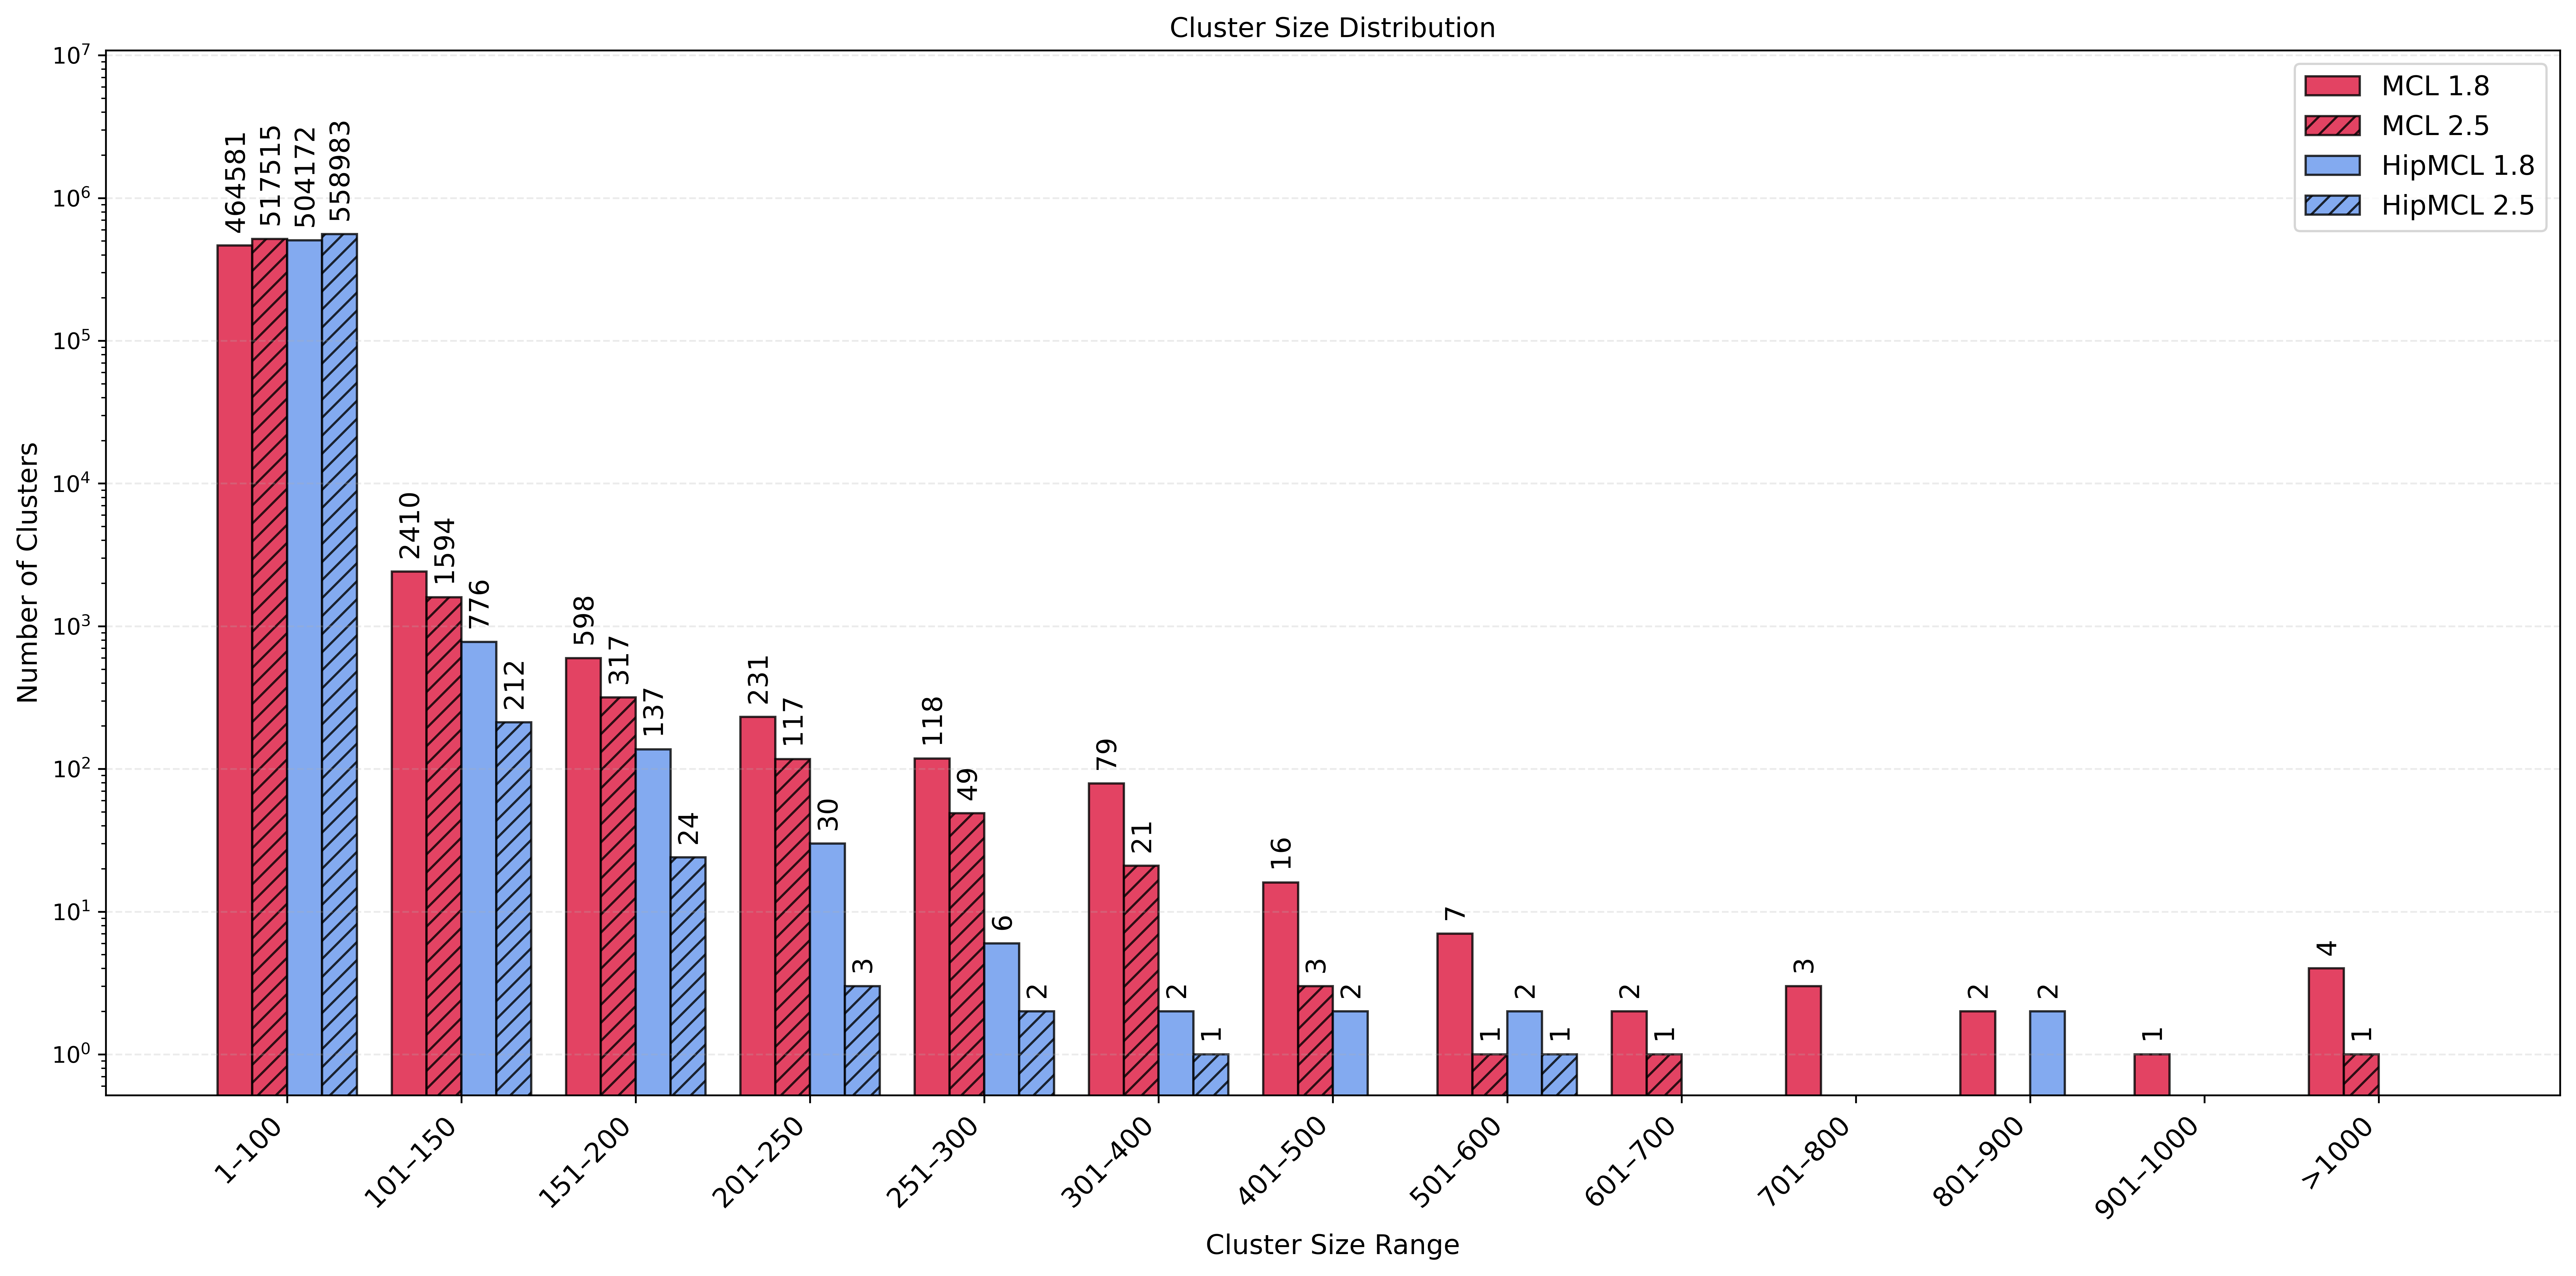
\includegraphics[width=\linewidth]{asset/cluster_size_distribution.png}
  \caption{Cluster size distribution on \texttt{bacteria\_tiny} (\(\sim\)3.0M
  proteins). The y-axis is logarithmic to reveal the heavy tail. MCL is shown in crimson, HipMCL in cornflower blue.}
  \label{fig:cluster_distr}
\end{figure}

% 700%
\begin{figure}[htbp]
  \centering
  \includegraphics[width=\linewidth]{asset/cluster_structures/partition_composition.png}
  \caption{In subfigures (a)--(i), three selected MCL clusters \texttt{r1},
  \texttt{r4} and \texttt{r22} from the \texttt{ref\_prot} dataset. Each row
  shows three randomly selected proteins from one cluster. For each cluster,
  each protein was selected with length near the cluster mean, and all three
  proteins collectively have non‑identical lengths. Ribbon coloring indicates
  per‑residue confidence (pLDDT). Subfigure (j) shows cluster size and
  taxonomic purity for the top‑25 clusters.}
  \label{fig:partition_composition}
\end{figure}

% 700%
\begin{figure}[htbp]
  \centering

  \includegraphics[width=\linewidth]{asset/cluster_structures/pairwise_structure_alignment.png}
  \caption{Subfigures (a)--(c) show superimposed ribbon diagrams of the
  selected proteins from Fig.~\ref{fig:partition_composition}, aligned using
  the \texttt{Matchmaker} command in UCSF ChimeraX \cite{chimerax}. Each
  cluster is colored uniquely (maroon, tan, purple). Subfigure (d) shows the
  adjacency matrix of the nine proteins based on percentage identity from
  BLASTp pairwise alignment.}

  \label{fig:pairwise_structure_alignment}
\end{figure}

  \cleardoublepage
  \section{Discussion}
\chead{\thesection. Discussion}

\subsubsection*{Sparsity as a Computational Enabler}

Only a tiny fraction of all possible protein pairs are preserved after
pairwise alignment and the subsequent E-value filtering: for the full \texttt{ref\_prot} dataset (82.1 million
proteins, 1.76 billion edges), the fraction of observed edges relative to a
complete graph is approximately \(5.2\text{e}-7\). This extreme sparsity makes
graph‑based clustering feasible on a single node, as it reduces both memory and
time complexity from \(\mathcal{O}(n^2)\) and \(\mathcal{O}(n^3)\) to
\(\mathcal{O}(n k_0)\) and \(\mathcal{O}(n k_0^2)\), respectively, where \(k_0
\approx 21\) is the average number of non‑trivial entries per column of the
adjacency matrix. The complexity analysis in the Background
(Observe Fig.~\ref{fig:complexity}) quantifies this advantage and is directly reflected
in the experimental runtimes: MCL completes within 2–3 days for the full
dataset using \(\sim 440\) GiB of memory, while a dense approach would
require petabytes of memory and years of computation.

\subsubsection*{Qualitative Characteristics of the Data and Clusters}

Frequency diagrams of amino acid compositions shown in Fig.~\ref{fig:aa_distr}
and sequence lengths of Fig.~\ref{fig:len_freq} provide a global signature of
each selected proteome but are not sufficient for clustering: they describe global
biases, not the pairwise relationships that determine cluster membership.
Additionally, from Fig.~\ref{fig:aa_distr}, the observed hydrophobic‑to‑charged
residue ratios range from 1.14 \textit{Danio rerio} (zebrafish) to 1.46
\textit{Carnobacterium maltaromaticum} (bacterium). To conveniently
discriminate between hydrophobic and charged residues, the reader can also view
the amino acid lookup table in Appendix~\ref{appendix:aminoAcidLookup}. 

Recent approaches have used learned embeddings from protein language models,
including TAPE~\cite{rao2019transformer}, ESM-2~\cite{lin2022esm2}, and
ProGen2~\cite{nijkamp2022progen2}, to represent sequences in Euclidean space.
While these methods achieve strong performance on some tasks, they trade off
interpretability and introduce large memory overhead. In contrast, the
graph‑based representation used here derives similarity directly from alignment
scores, preserving biological meaning without black‑box abstraction.

With this graph‑based representation, the resulting clusters can be directly
interpreted by examining their taxonomic composition and structural coherence.
The three largest clusters each consist predominantly of proteins from the same
organism \textit{Austropuccinia psidii MF-1}, (rust fungus) with TaxID 01389203
a strain from a species that causes myrtle rust in various plants.
\textit{Austropuccinia psidii} (myrtle rust) is a pathogen of Myrtaceae plants
\cite{psidii}. This can be observed in the bar plot of
Fig.~\ref{fig:partition_composition} (j), showing the top-25 clusters ranked
from largest to smallest. Hence, this suggests that this organism possesses
unusually large and diverse protein families, each large enough to form a top
cluster. Other organisms appear primarily in smaller clusters, indicating
either lower representation in the dataset or less internal sequence diversity.
Purity values are high across the top‑25 clusters, indicating that MCL tends to
group proteins that match the biological profile of a limited set of dominant
organisms, especially in the largest clusters.

\subsubsection*{Algorithmic Behaviour: Granularity and Differences Between MCL and HipMCL}

Higher inflation consistently produces more clusters than lower inflation as
shown in Table~\ref{tab:experimentsPalladium} and, for datasets up to 35
million proteins, also reduces runtime. This matches MCL's design: inflation
strengthens dominant connections, accelerates convergence, and yields finer
granularity. The cluster size distribution (Fig.~\ref{fig:cluster_distr})
partially supports this premise: the distribution moves towards smaller
clusters when inflation is set to 2.5 for both algorithms.

Although MCL and HipMCL share the same core algorithm, HipMCL consistently
produces slightly more clusters at the same inflation value, likely due to
differences in pruning strategies or numerical precision. However, its memory
overhead (2–4 times higher than MCL) and convergence issues make it impractical
for single‑node runs on datasets larger than 3 million sequences. This does not
diminish HipMCL's value; it was designed for distributed environments, where it
excels.

\subsubsection*{Reproducibility and Random Walks}

Both MCL and HipMCL rely on random walks that simulate flow in the graph, but
their implementations differ in pruning strategies, numerical precision, and
convergence criteria. Table~\ref{tab:experimentsPalladium} shows that for the
same inflation, direct quantitative comparison of individual clusters between
MCL and HipMCL is inherently ambiguous.

However, this does not compromise the reproducibility of the present work. The
reported metrics --- runtime, peak memory, number of clusters, cluster size
distributions, and taxonomic purity --- are all stable across runs. Moreover,
the exact clusters produced by each algorithm can be reproduced by fixing the
input graph and using the same software versions (commit digests) and
parameters. The workflow is implemented in \texttt{bioscflow}, a Python
codebase that orchestrates GeneCAST, DIAMOND, MCL, and HipMCL (observe
Fig.~\ref{fig:workhigh}), manages file paths and intermediate data, and
systematically records execution logs and runtime metrics in JSON session
reports which is particularly useful when producing multiple experiments. The
observed differences in cluster counts and granularity between MCL and HipMCL
are therefore meaningful as algorithmic characteristics, even if individual
cluster assignments are not
directly comparable.

\subsubsection*{Limitations}

Three main limitations should be noted. First, HipMCL was tested only in
single‑node mode; its poor performance here does not reflect its capabilities
on large clusters. Second, biological validation of individual clusters was
outside the scope of this work. Third, the reference proteome dataset, while
large, is biased toward well‑studied organisms, and the chosen BLASTp
thresholds may not be optimal for every application.

Another major limitation concerns the stochastic nature of the random walks
underlying both MCL and HipMCL. Because the algorithms rely on simulated flow,
runtime measurements may exhibit non‑deterministic fluctuations. In principle,
a larger input could occasionally complete faster than a smaller input in a
single run, potentially obscuring true scaling behavior. All reported runtimes
are based on single executions; therefore, the observed trends should be
interpreted with caution. Systematic averaging over multiple runs with
different random seeds would be required to obtain statistically reliable scaling
estimates.

\subsubsection*{Design Priorities Revisited}

The workflow meets the three priorities set in the Introduction, namely
\textit{Scalability}: MCL processed 82 million sequences on a single node.
\textit{Reproducibility}: the entire pipeline is implemented in
\texttt{bioscflow} with versioned tools and commits. \textit{Interpretability}:
graph edges are derived directly from alignment scores, avoiding black‑box
embeddings.

  \cleardoublepage
  \section[Conclusion \& \ Future Work]{Conclusion \& Future Work}
\chead{\thesection. Conclusion \& Future Work}

This thesis investigated the practical scalability of the Markov Clustering
Algorithm (MCL) and its high‑performance variant HipMCL for protein sequence
similarity networks on a single compute node. Using datasets ranging from
20,000 to 82 million protein sequences from reference proteomes, we established
a clear computational baseline.

The key findings are:

\begin{enumerate}
  \item \textbf{MCL scales to 82 million sequences} on a single node, completing in 2–3 days with \(\sim\) 440 GiB of memory. The observed runtime and memory usage follow the expected \(\mathcal{O}(n k_0^2)\) complexity, enabled by extreme graph sparsity.
  \item \textbf{HipMCL is not suitable for single‑node use} beyond 3 million sequences; its memory overhead and convergence issues lead to failures within a 4‑day limit.
  \item \textbf{Cluster quality is appropriate}: Clusters are taxonomically pure (overall purity 0.96) and structurally coherent, as confirmed by AlphaFold structure superimposition.
  \item \textbf{Inflation controls granularity}: Higher inflation arguments (2.5) produce finer clusters compared to lower ones (1.8), with faster convergence on most datasets.
\end{enumerate}

These results provide a green light for scaling the StratoCluster pipeline to cloud environments.

\subsubsection*{Future Work}

Building on this baseline, three directions are planned:

\begin{enumerate}
  \item \textbf{Statistical characterization}: Perform Monte Carlo simulations on synthetic sequence datasets of controlled size and sparsity to average out stochastic fluctuations and obtain reliable runtime estimates.
  \item \textbf{GPU acceleration}: Parallelize the all‑vs‑all alignment and graph construction steps using CUDA to reduce preprocessing time.
  \item \textbf{Distributed execution}: Deploy HipMCL in its intended distributed configuration using MPI across multiple nodes to process the full 12,000‑proteome sequence set.
\end{enumerate}

The single‑node baseline established here is a necessary prerequisite for these
larger‑scale efforts and serves as a foundation for future benchmark studies,
e.g., comparison with other state‑of‑the‑art clustering workflows.

  \cleardoublepage
  \section*{Appendices}
\chead{Appendices}

\phantomsection
\addcontentsline{toc}{section}{Appendices}

\appendix
\appendixsec{Molecule Lookup Tables}
\label{appendix:aminoAcidLookup}
\renewcommand{\thefigure}{A\arabic{figure}}
\renewcommand{\thetable}{A\arabic{table}}
\setcounter{figure}{0}
\setcounter{table}{0}

\begin{table}[htbp]
  \centering
  \begin{minipage}{0.58\linewidth}
    \centering
    \captionof{table}{Amino acid codes. Selenocysteine (\texttt{U}) and pyrrolysine (\texttt{O}) are non-standard. Hydrophobic (\textbf{H}) and Charged (\textbf{C}) properties are indicated with \ding{51} (yes) or \textcolor{gray}{\ding{53}} (no).}
    \begin{tabular}{clcc}
      \toprule
      \textbf{1-letter} & \textbf{Full Name} & \textbf{H} & \textbf{C} \\
      \midrule
      \texttt{A} & Alanine & \ding{51} & \textcolor{gray}{\ding{53}} \\
      \texttt{R} & Arginine & \textcolor{gray}{\ding{53}} & \ding{51} \\
      \texttt{N} & Asparagine & \textcolor{gray}{\ding{53}} & \textcolor{gray}{\ding{53}} \\
      \texttt{D} & Aspartic acid & \textcolor{gray}{\ding{53}} & \ding{51} \\
      \texttt{C} & Cysteine & \ding{51} & \textcolor{gray}{\ding{53}} \\
      \texttt{E} & Glutamic acid & \textcolor{gray}{\ding{53}} & \ding{51} \\
      \texttt{Q} & Glutamine & \textcolor{gray}{\ding{53}} & \textcolor{gray}{\ding{53}} \\
      \texttt{G} & Glycine & \textcolor{gray}{\ding{53}} & \textcolor{gray}{\ding{53}} \\
      \texttt{H} & Histidine & \textcolor{gray}{\ding{53}} & \ding{51} \\
      \texttt{I} & Isoleucine & \ding{51} & \textcolor{gray}{\ding{53}} \\
      \texttt{L} & Leucine & \ding{51} & \textcolor{gray}{\ding{53}} \\
      \texttt{K} & Lysine & \textcolor{gray}{\ding{53}} & \ding{51} \\
      \texttt{M} & Methionine & \ding{51} & \textcolor{gray}{\ding{53}} \\
      \texttt{F} & Phenylalanine & \ding{51} & \textcolor{gray}{\ding{53}} \\
      \texttt{P} & Proline & \ding{51} & \textcolor{gray}{\ding{53}} \\
      \texttt{S} & Serine & \textcolor{gray}{\ding{53}} & \textcolor{gray}{\ding{53}} \\
      \texttt{T} & Threonine & \textcolor{gray}{\ding{53}} & \textcolor{gray}{\ding{53}} \\
      \texttt{W} & Tryptophan & \ding{51} & \textcolor{gray}{\ding{53}} \\
      \texttt{Y} & Tyrosine & \ding{51} & \textcolor{gray}{\ding{53}} \\
      \texttt{V} & Valine & \ding{51} & \textcolor{gray}{\ding{53}} \\
      \midrule
      \texttt{U} & Selenocysteine & \textcolor{gray}{\ding{53}} & \textcolor{gray}{\ding{53}} \\
      \texttt{O} & Pyrrolysine & \textcolor{gray}{\ding{53}} & \textcolor{gray}{\ding{53}} \\
      \bottomrule
    \end{tabular}
    \label{tab:amino_acids}
  \end{minipage}
  \hfill
  \begin{minipage}{0.40\linewidth}
    \centering
    \captionof{table}{DNA residues.}
    \begin{tabular}{cl}
      \toprule
      \textbf{1-letter} & \textbf{Full Name} \\
      \midrule
      \texttt{A} & Adenine \\
      \texttt{C} & Cytosine \\
      \texttt{G} & Guanine \\
      \texttt{T} & Thymine \\
      \bottomrule
    \end{tabular}
    \label{tab:dna}

    \vspace{0.5cm}

    \centering
    \captionof{table}{RNA residues.}
    \begin{tabular}{cl}
      \toprule
      \textbf{1-letter} & \textbf{Full Name} \\
      \midrule
      \texttt{A} & Adenine \\
      \texttt{C} & Cytosine \\
      \texttt{G} & Guanine \\
      \texttt{U} & Uracil \\
      \bottomrule
    \end{tabular}
    \label{tab:rna}
  \end{minipage}
\end{table}

\appendix
\appendixsec{Stochasticity Preservation of Exponentiated Matrices}
\label{appendix:proofExp}

\textbf{Theorem}. Suppose \(\mathcal{M}\) is any square matrix with real entries where each column is a discrete probability distribution (PD). Then for every \(e \in \mathbb{N}^*\), each column of \(\mathcal{M}^e\) is a PD as well.

\textit{Proof}

To justify the aforementioned proposition, the following proof method will rely on mathematical induction. Define the proposition \(h_{e}\) as
\[
  \sum_{j = 1}^{n} (\mathcal{M}^e)_{j, k} = 1 \ \left( \forall k \in \{ 1, \dots, n \} \right).
\]
The base case \(h_1\) (for \(e:=1\)) holds, since all columns of \(\mathcal{M}^1\) are already PDs. Now it suffices to prove that \(h_{e}\) implies \(h_{e+1}\).

Accordingly, for some arbitrary \(e \in \mathbb{N}^{*}\), the proposition \(h_e\) is assumed to be true. Given this premise, to confirm that \(h_{e+1}\) holds, fix \(k \in \{ 1, \dots, n \}\) and compute the sum
\begin{align*}
  \sum_{j=1}^{n} ( \mathcal{M}^{e+1} )_{j,k}
  & = \sum_{j=1}^{n} \left( \sum_{q=1}^{n} ( (\mathcal{M}^{e})_{j,q} \cdot \mathcal{M}_{q,k} ) \right)
  \\
  & = \sum_{q=1}^{n} \left( \sum_{j=1}^{n} \left( (\mathcal{M}^{e})_{j,q} \cdot \mathcal{M}_{q,k} \right) \right)
  \\
  & = \sum_{q=1}^{n} \left( \sum_{j=1}^{n} \left( \mathcal{M}_{q,k} \cdot (\mathcal{M}^{e})_{j,q} \right) \right)
  \\
  & = \sum_{q=1}^{n} \left( \mathcal{M}_{q,k} \cdot \sum_{j=1}^{n} (\mathcal{M}^{e})_{j,q} \right)
  \\
  & \overset{h_{e}}{=} \sum_{q=1}^{n} ( \mathcal{M}_{q,k} \cdot 1 )
  \\
  & = \sum_{q=1}^{n} \mathcal{M}_{q,k}
  \\
  & \overset{h_{1}}{=} 1.
\end{align*}
Subsequently, by induction, the proposition \(h_{e}\) holds for all \(e \in \mathbb{N}^*\).

Also, since \(\mathcal{M}_{j,k} \in [0, 1]\), notice that \((\mathcal{M}^e)_{j,k} > 0\). Suppose there exists a pair \(j_0, k_0 \in \{ 1, \dots, n \}\) such that \((\mathcal{M}^{e})_{j_0, k_0} > 1\). Then since \((\mathcal{M}^e)_{j, k_0} > 0\) for all \(j \in \{ 1, \dots, n \}\), we have that
\[
  \sum_{j=0}^{n} (\mathcal{M}^{e})_{j, k_0} > 1
\]
which is impossible since it contradicts \(h_e\); hence no such pair \(j_0, k_0\) can exist. Therefore, for all \(j, k \in \{ 1, \dots, n \}\), it is
\[
  (\mathcal{M}^{e})_{j, k} \in [0, 1] .
\]

\(\blacksquare\)

  \cleardoublepage

  % ===== Reference =====

  \bibliographystyle{IEEEtran}
  \bibliography{ref}
  \phantomsection
  \addcontentsline{toc}{section}{References}

\end{document}
